%%
%% Copyright 2019-2021 Elsevier Ltd
%%
%% This file is part of the 'CAS Bundle'.
%% --------------------------------------
%%
%% It may be distributed under the conditions of the LaTeX Project Public
%% License, either version 1.2 of this license or (at your option) any
%% later version.  The latest version of this license is in
%%    http://www.latex-project.org/lppl.txt
%% and version 1.2 or later is part of all distributions of LaTeX
%% version 1999/12/01 or later.
%%
%% The list of all files belonging to the 'CAS Bundle' is
%% given in the file `manifest.txt'.
%%
%% Template article for cas-sc documentclass for
%% single column output.

\documentclass[a4paper,fleqn]{cas-sc}

% If the frontmatter runs over more than one page
% use the longmktitle option.

%\documentclass[a4paper,fleqn,longmktitle]{cas-sc}

\usepackage[numbers]{natbib}
%\usepackage[authoryear]{natbib}
%\usepackage[authoryear,longnamesfirst]{natbib}
%%%Author macros
\def\tsc#1{\csdef{#1}{\textsc{\lowercase{#1}}\xspace}}
\tsc{WGM}
\tsc{QE}
%%%

% Uncomment and use as if needed
%\newtheorem{theorem}{Theorem}
%\newtheorem{lemma}[theorem]{Lemma}
%\newdefinition{rmk}{Remark}
%\newproof{pf}{Proof}
%\newproof{pot}{Proof of Theorem \ref{thm}}

\begin{document}
\let\WriteBookmarks\relax
\def\floatpagepagefraction{1}
\def\textpagefraction{.001}

% Short title
\shorttitle{Impact of Iron Defect Variability on Silicon Solar Cell Performance}

% Short author
\shortauthors{O.Olikh, O.Zavhorodnii}

% Main title of the paper
\title [mode = title]{Modeling the Impact of Iron Defect Variability on Silicon Solar Cell Performance Across Different Scenarios}

% Title footnote mark
% eg: \tnotemark[1]
%\tnotemark[<tnote number>]

% Title footnote 1.
% eg: \tnotetext[1]{Title footnote text}
%\tnotetext[<tnote number>]{<tnote text>}

% First author
%
% Options: Use if required
% eg: \author[1,3]{Author Name}[type=editor,
%       style=chinese,
%       auid=000,
%       bioid=1,
%       prefix=Sir,
%       orcid=0000-0000-0000-0000,
%       facebook=<facebook id>,
%       twitter=<twitter id>,
%       linkedin=<linkedin id>,
%       gplus=<gplus id>]

%\author[1,3]{Oleg Olikh}[type=Co-ordinator,
%       style=chinese,
%       auid=000,
%       bioid=1,
%       prefix=Dr.,
%       orcid=0000-0003-0633-5429,
%%       facebook=<facebook id>,
%%       twitter=<twitter id>,
%%       linkedin=<linkedin id>,
%       gplus=<gplus id>]
\author{Oleg Olikh}[
%       type=Co-ordinator,
%       style=chinese,
%       auid=000,
%       bioid=1,
%       prefix=Dr.,
       orcid=0000-0003-0633-5429
       % ,
%       facebook=<facebook id>,
%       twitter=<twitter id>,
%       linkedin=<linkedin id>,
%       gplus=<gplus id>
       ]

% Corresponding author indication
\cormark[1]

% Footnote of the first author
%\fnmark[1]

% Email id of the first author
\ead{olegolikh@knu.ua}

% URL of the first author
%\ead[url]{https://gen.phys.univ.kiev.ua/280-olikh/}

% Credit authorship
% eg: \credit{Conceptualization of this study, Methodology, Software}
%\credit{<Credit authorship details>}

% Address/affiliation
\affiliation{organization={Taras Shevchenko National University of Kyiv},
            addressline={64/13, Volodymyrska Street},
            city={Kyiv},
%          citysep={}, % Uncomment if no comma needed between city and postcode
            postcode={01601},
 %           state={},
            country={Ukraine}}

%\affiliation[<aff no>]{organization={Taras Shevchenko National University of Kyiv, Faculty of Physics},
%            addressline={ave Glushkov 2},
%            city={Kyiv},
%%          citysep={}, % Uncomment if no comma needed between city and postcode
%            postcode={03022},
%            state={},
%            country={Ukraine}}

%\author[1,3]{Zavhorodnii Oleksii}[type=editor,
%       style=chinese,
%       auid=000,
%       bioid=1,
%%       prefix=Mr,
%       orcid=0000-0001-8080-7661,
%%       facebook=<facebook id>,
%%       twitter=<twitter id>,
%%       linkedin=<linkedin id>,
%       gplus=<gplus id>]

\author{Oleksii Zavhorodnii}[
       orcid=0000-0001-8080-7661]

% Footnote of the second author
%\fnmark[2]

% Email id of the second author
\ead{nevermor464@gmail.com}

% URL of the second author
%\ead[url]{https://gen.phys.univ.kiev.ua/}

% Credit authorship
%\credit{}

% Address/affiliation
%\affiliation[<aff no>]{organization={Taras Shevchenko National University of Kyiv, Faculty of Physics},
%            addressline={ave Glushkov 2},
%            city={Kyiv},
%%          citysep={}, % Uncomment if no comma needed between city and postcode
%            postcode={03022},
%            state={},
%            country={Ukraine}}

% Corresponding author text
%\cortext[1]{Corresponding author}

% Footnote text
%\fntext[1]{}

% For a title note without a number/mark
%\nonumnote{}

% Here goes the abstract
\begin{abstract}
The transition to renewable energy sources is paramount for mankind's sustainable development, and silicon solar cells are at the forefront of solar energy conversion. This study examines the impact of iron defect variability on silicon solar cell performance across various scenarios, integrating modeling and experimental validation. We conducted simulations using SCAPS software across a range of temperatures $(290-340)$~K, base thicknesses $(180-380)$~$\mu$m, doping levels ($10^{15} - 10^{17}$)~cm$^{-3}$, with iron concentrations varying from $10^{10}$ to $10^{14}$~cm$^{-3}$ under AM1.5 and monochromatic (940~nm) illumination. The dissociation of iron-boron pairs and its effects on short-circuit current, open-circuit voltage, fill factor, and efficiency were analyzed. The experimental measurements validated the simulation results, demonstrating good agreement with the main photovoltaic parameters. The study's findings contribute to the development of practical methods for assessing iron contamination in silicon solar cells using standard $I$-$V$ measurements, offering a pathway to improving the efficiency and reliability of these devices.
\end{abstract}

% Use if graphical abstract is present
%\begin{graphicalabstract}
%\includegraphics{}
%\end{graphicalabstract}

% Research highlights
\begin{highlights}
\item Short-circuit current changes are most suitable for estimating iron impurity concentration.
\item Open-circuit voltage changes non-monotonic at low boron doping levels.
\item Efficiency and open-circuit voltage changes are useful but limited at low doping levels.
\item Fill factor least suitable for estimating iron impurity concentration.
\item Monochromatic illumination is more effective than AM1.5 for accurate iron concentration estimation.
% \item Accuracy of iron concentration estimation depends on base doping level and illumination intensity.
\end{highlights}



% Keywords
% Each keyword is seperated by \sep
\begin{keywords}
 silicon\sep iron-boron pairs\sep solar cells \sep SCAPS \sep simulation \sep defect influence
\end{keywords}

\maketitle

% Main text
\section{Introduction}%\label{}
\par
The necessity for renewable energy sources to meet the growing global demand for sustainable and environmentally friendly energy alternatives has become evident.
Among the wide range of renewable energy sources, sunlight is the cleanest, safest,
and most abundant source for use in sustainable energy to support economic growth \cite{PratapSingh2019}.
The utilization of solar energy heavily depends on the use of photovoltaic cells, with silicon--based devices playing a critical role \cite{Basnet2024,Wang2024}.


The issue of semiconductor purity has become increasingly significant since the advent of the transistor in 1947 \cite{Claers2018}.
The 1960 study by Shockley and Queisser \cite{Goetzberger1960} demonstrated that
the electrical properties of $n^{+}-p$ silicon diodes deteriorate when impurity atoms of metals such as Cu, Fe, Mn, Au, Zn, and Ni are present.
This study prompted investigations focused on preventing contaminating metals from entering semiconductors during manufacturing.
In particular, metallic impurities are known to reduce the efficiency of
silicon--based devices through direct shunting \cite{Rsh:Breitenstein},
increased leakage current \cite{Lee1980},
or bulk recombination \cite{Istratov2000}.
Despite extensive study of metallic impurities in silicon over the past fifty years \cite{Claers2018,Pearce1977},
the problem continues to attract significant attention \cite{Hajjiah2020,Le2024,Maoudj2021,OlikhPSSA,LaineIEEEPV2016}.


Iron is prominent among metallic contaminants, with its atoms being among
the most prevalent and detrimental impurities in silicon solar cells (SSCs) \cite{Buonassisi2006}.
Even in small concentrations (about $10^{10}$~cm$^{-3}$),
point defects related to Fe can significantly influence the performance of SSCs \cite{IronSC,Herguth2022}.
Therefore, it is of critical importance to assess the concentration of iron impurities.
In response to this challenge, various methodologies have been put forward,
often based on the property of iron atoms to form pairs with acceptors.
In particular, iron atoms are predominantly located in interstitial positions in silicon, forming the Fe$_i$ defect.
In $p$--type crystals, without external illumination, iron atoms carry positive charges and tend to bond with negatively charged doping atoms
(boron, aluminum, gallium, or indium), forming Fe$_i$B$_\mathrm{Si}$ pairs \cite{Kimerling1983}.
However, these pairs can destabilized by intense illumination, electron injection, or heating up to 200~$^\circ$C \cite{FeBAssJAP2014}.
The recombination properties of iron-related defects Fe$_i$ and Fe$_i$B$_s$ differ significantly,
which profoundly affects the overall characteristics of the crystal.
This fact formed the basis for the first method of assessing iron concentration \cite{Zoth1990},
which relied on measuring the diffusion length of minority carriers using the surface photovoltage method \cite{Tousek2008}.
Many other methods involve measurements of carrier lifetime \cite{Rein2,Schmidt2005},
Quasi-Steady-State Photoconductance \cite{Goodarzi2017},
or the study of kinetic dependencies of short-circuit current \cite{Olikh2021JAP}
or photoluminescence intensity \cite{FeMethod2012} during the reaction Fe$_i$B$_\mathrm{Si}$ $\rightleftarrows$ Fe$_i$ + B$_\mathrm{Si}$.


Notably, the presence of Fe--related defects affects the dynamics of electron and hole movement within the solar cell,
which is reflected in changes to the appearance of the current--voltage ($I$-$V$) characteristics of SSCs overall,
as well as modifications to the main photoelectric parameters
(short-circuit current  $I_\mathrm{SC}$,
open-circuit voltage $V_\mathrm{OC}$,
efficiency $\eta$, and fill factor $FF$)
in particular.
These findings create fundamental possibilities to advance methods for estimating iron concentration by $I$-$V$ curves measuring before and after pair dissolution.
The advantages of such an approach are associated with the possibility of directly characterizing finished solar cells,
as well as the absence of the need for additional equipment other than that required for $I$-$V$ measurements, which is extremely common.
Efforts have been made initially in developing such methods.
For instance, it was proposed to estimate the concentration of iron in SSCs based on changes in the ideality factor \cite{Olikh2019SM,Olikh2022PPV}
or open-circuit voltage \cite{Herguth2022}.
However, developing such approaches requires evaluating how a particular parameter changes when iron--containing pairs dissolve
and determining whether it can estimate the iron concentration $N_\mathrm{Fe}$.
For example, the most evident conditions for utilizing a specific parameter include its change due to the transformation
Fe$_i$B$_\mathrm{Si}$ $\rightarrow$ Fe$_i$ +B$_\mathrm{Si}$,
at least by 10\%, along with a monotonic dependence of these changes on $N_\mathrm{Fe}$.


This paper intends to determine the variations of $I_\mathrm{SC}$, $V_\mathrm{OC}$, $\eta$, and $FF$
resulting from the decay of iron-containing pairs in boron-doped silicon solar cells.
Previous similar calculations have been conducted \cite{FeB:Schmidt,IronSC,Hajjiah2020},
but the results presented typically pertain only to certain temperatures,
illumination levels (often AM1.5), and solar cells with specific parameters.
In this study, we performed calculations over a sufficiently wide temperature range (290-340~K)
and for solar cells with varying base thickness (180-380~$\mu$m) and doping levels
(boron concentration in the base ranging from $10^{15}$ to $10^{17}$~cm$^{-3}$).
The results obtained allow us to assess the feasibility and potential of using the
main photovoltaic parameters of specific solar cells to estimate the $N_\mathrm{Fe}$ value across a range of temperatures,
including conditions similar to those encountered in typical SSC applications.
Furthermore, investigations have explored changes in photoelectric performance under not only solar illumination (AM1.5G)
but also low-intensity monochromatic light (wavelength of 940~nm, intensities of 5~W/m$^{2}$ and 10~W/m$^{2}$).
In the first case, while it is customary to adhere to standard conditions,
it's essential to consider that illumination at 1000~W/m$^{2}$ can lead to the decay of Fe$_i$B$_s$ complexes \cite{Macdonald2004}.
Therefore, measurements for cases requiring the presence of undissociated pairs in silicon must meet specific constraints.
On the other hand, intentionally chosen monochromatic illumination penetrates the emitter with negligible losses and does not reach the rear side.
In this context, the photoelectric parameters show remarkable sensitivity
to recombination processes occurring within the solar cell base and to iron concentration in this region.
Finally, in our calculations, we attempted to use the latest literature data
concerning the exact values of silicon parameters, including light absorption values \cite{Green2022}
and coefficients characterizing intrinsic recombination \cite{Brad2022,AugerSi2022}.

\section{Research Methodology}%\label{}

\subsection{Simulation Details}
The study involved simulation $I$-$V$ curves of SSCs with an $n^+-p-p^+$ structure,
as illustrated in Fig.~\ref{fig1}.
A back surface field ($p^+$-layer) is a notable feature observed in both Al-BSF cells (full area),
which are gradually losing relevance,
and PERC cells (locally), which are the most widely used in mass production.
The structures with a base uniformly doped with boron were under consideration.
The doping concentration $N_\mathrm{B}$, and the base thickness $d_p$ were varied during the modeling process, as detailed in Table~\ref{table1}.
The emitter and $p^+$-layer were considered to be unevenly doped.
The concentration profiles of the dopants, their maximum values ($N_{p^+,\mathrm{max}}$ and $N_{n^+,\mathrm{max}}$),
and layer thicknesses (see Fig.~\ref{fig1}) were selected according to Fell et al. \cite{Fell2015}.


\begin{figure}
	\centering
		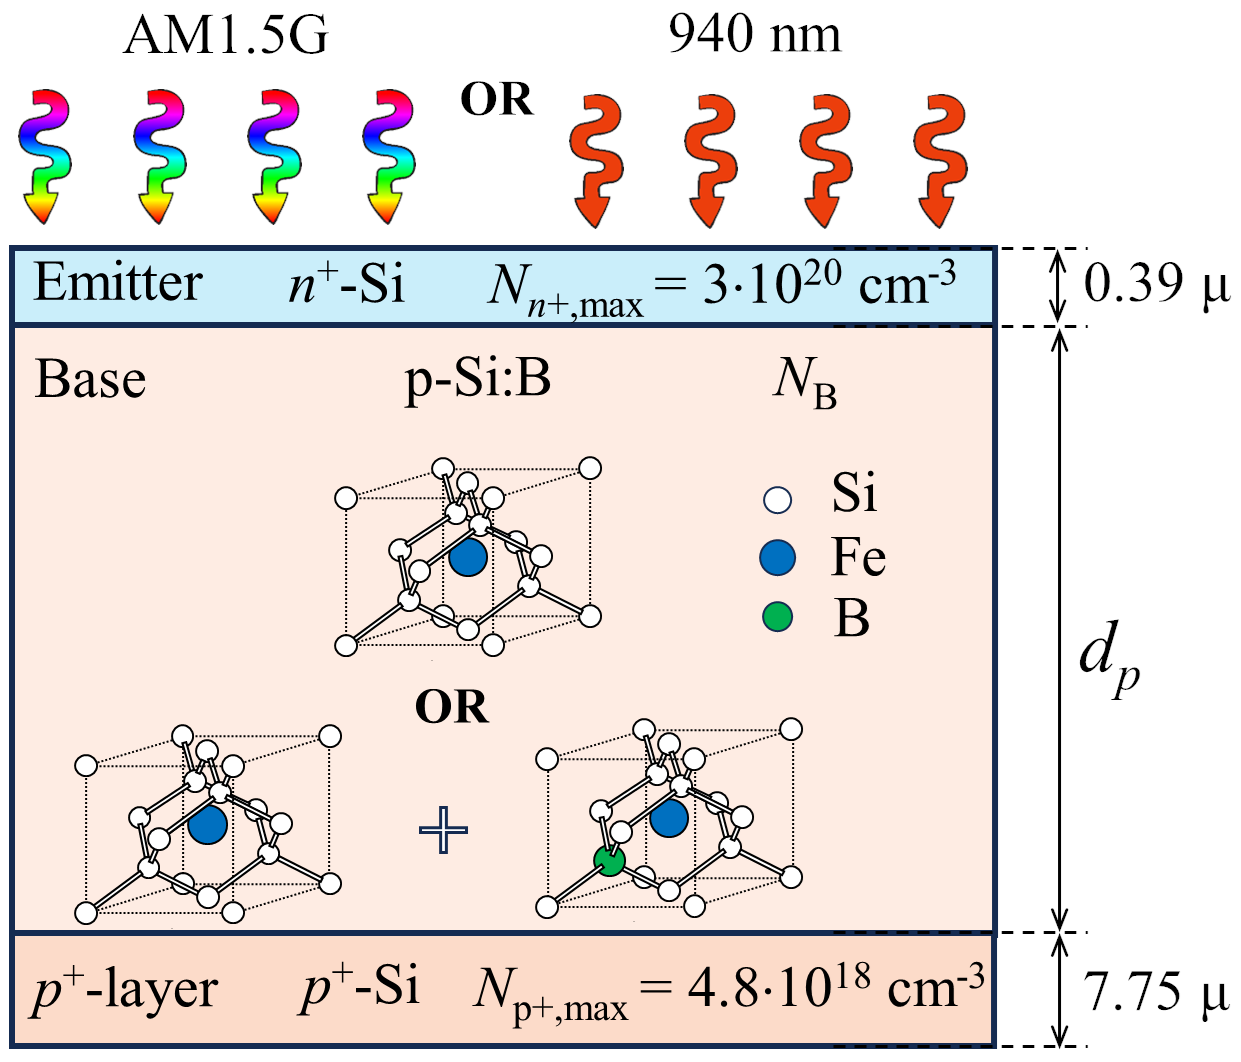
\includegraphics[width=0.5\linewidth]{Figure1.png}
	  \caption{Schematic diagram of analyzed solar cells.}\label{fig1}
\end{figure}


\begin{table}
\caption{Parameters varied during the simulation}\label{table1}
\begin{tabular*}{\tblwidth}{@{}LL@{}}
\toprule
  Parameter & Range of values \\ % Table header row
\midrule
 $d_p$($\mu$m)   & $180-380$\\
 $N_\mathrm{B}$ (cm$^{-3}$)    & $10^{15} - 10^{17}$\\
 $N_\mathrm{Fe}$ (cm$^{-3}$) & $10^{10} - 10^{14}$\\
 $T$ (K)                        & $290 - 340$\\
 Illumination                 & AM1.5G, 1000~W/$\mathrm{m}^{2}$; \\
 & 940~$\mathrm{nm}$, 5~W/$\mathrm{m}^{2}$; 940~$\mathrm{nm}$, 10~W/$\mathrm{m}^{2}$\\
\bottomrule
\end{tabular*}
\end{table}


The simulation was conducted using the SCAPS~3.3.11 code \cite{SCAPS1}.
SCAPS-1D software, developed by the University of Gent, is founded on theoretical computations that involve solving Poisson's equation,
continuity equations for holes and electrons, and drift-diffusion at each position within the solar cell,
considering the boundary conditions.
Despite its one-dimensional modeling approach, SCAPS is extensively used for modeling various types of solar cells \cite{Joshi2024,Ravidas2024,Liu2024,You2023} in general
and for investigating the effects of defects on their performance \cite{AitAbdelkadir2023,Liang2024,SCAPSDefect3} in particular.


As can be seen from Table~\ref{table1}, calculations spanned a broad range of temperatures and base doping levels.
Therefore, to improve the accuracy of the calculations when inputting the initial parameters into SCAPS,
temperature and concentration (where applicable) dependencies of the following silicon parameters were taken into account:

\begin{itemize}
    \item bandgap according to Passler \cite{Passler2002};
    \item doping induced bandgap narrowing according to Yan \& Cuevas \cite{EgNarrow};
    \item effective density of states at conduction and valence band and intrinsic carrier concentration according to Couderc et al. \cite{Si_ni_Couderc};
    \item thermal carrier velocities according to Green \cite{Nc:Green};
    \item free carrier effective masses according to O’Mara et al. \cite{OMara};
    \item carrier mobilities according to Klaassen's theory \cite{KLAASSEN953};
\end{itemize}

The values of surface recombination coefficients were considered equal to the thermal velocities of carriers \cite{Fell2015}.
The calculations addressed recombination processes within the structural volume,
incorporating both intrinsic recombination and Shockley-Read-Hall recombination at iron-related defects.
In the first case, processes of band-to-band radiation recombination were considered
(where the calculation of the corresponding coefficient included the fraction of radiatively emitted photons
reabsorbed via band-to-band processes according to Niewelt et al.\cite{Brad2022})
and Auger recombination (where the coefficients considered the effect of Coulomb enhancement \cite{AugerSi2022} and temperature dependence \cite{Si_Auger}).


When accounting for the influence of iron impurities,
we considered that Fe atoms were uniformly distributed within the base and $p^+$-layer
with a total concentration of $N_\mathrm{Fe}$ (see Table~\ref{table1}).
Two cases were under consideration:

Case~1.
The concentration of interstitial iron defects $\left[\mathrm{Fe}_i\right]=N_\mathrm{Fe}$  at each position throughout the solar cell,
with no pairs present $\left[\mathrm{Fe}_i\mathrm{B}_s\right]=0$.
This case corresponds to the state of the structure immediately after intense illumination, for example.

Case~2.
Iron atoms predominantly form pairs with acceptors, $\left[\mathrm{Fe}_i\mathrm{B}_s\right] \gg \left[\mathrm{Fe}_i\right]$,
but the exact concentration ratio depends on the position of the Fermi level and temperature \cite{FeB:kinetic,MurphyJAP2011}
and varies from point to point within the solar cell.
Further details about calculation of the concentration profiles of Fe$_i$B$_s$ and Fe$_i$ are provided in \cite{Olikh2022PPV,Olikh2019SM}.
This case corresponds to prolonged storage of the structure in darkness or under conditions of low-intensity ($< 0.01$~J~cm$^{-2}$ \cite{Macdonald2004}) illumination.


During the calculations, it was assumed that Fe$_i$ forms a single donor level,
while the Fe$_i$B$_s$ pair has a trigonal configuration and acts as an amphoteric defect.
We obtained defect parameters (including level positions within the bandgap and electron and hole capture cross-sections) from relevant studies \cite{ROUGIEUX2018,Istratov1999,Paudyal}.

As previously mentioned, the solar cell behavior was simulated under different illumination conditions,
including solar light (AM1.5G) and monochromatic light (wavelength 940~nm, intensity of $W_\mathrm{ill} = 5$~Wm$^{-2}$ or 10~W/$\mathrm{m}^{2}$) --– see Table~\ref{table1}.
The calculations incorporated the light absorption values in silicon based on Green's study \cite{Green2022}.


The $I$-$V$ characteristics were simulated for both Case~1 and Case~2 (see Fig.~\ref{fig2}),
and from each curve, the short-circuit current, open-circuit voltage, efficiency, and fill factor were determined.
Assessing the influence of iron defect variability relied on the relative changes in each photovoltaic conversion parameter:

\begin{figure}
	\centering
		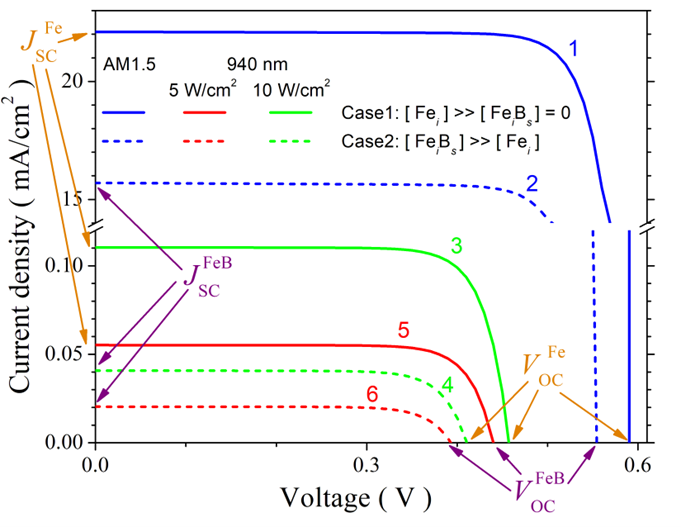
\includegraphics[width=0.5\linewidth]{Figure2.png}
	  \caption{Typical IV characteristics,
   calculated for structure with $d_p = 180$~$\mu$m, $N_\mathrm{B}=10^{17}$~cm$^{-3}$,
   $N_\mathrm{Fe}=10^{14}$~cm$^{-3}$ at $T = 290$~K.
   Illumination: AM1.5 (curves 1, 2), 940~nm 10~Wcm$^{-2}$ (3, 4) and 940~nm 5~Wcm$^{-2}$ (5, 6).
   Solid and dotted lines correspond to Case~1 and Case~2, respectively.}\label{fig2}
\end{figure}


\begin{equation}
\label{eq1}
    \varepsilon A = \frac{A^\mathrm{FeB} - A^\mathrm{Fe}}{A^\mathrm{FeB}} \times 100 \%\,,
\end{equation}
where $A$ represents one of the parameters ($I_\mathrm{SC}$, $V_\mathrm{OC}$, $\eta$, and $FF$),
superscript ‘‘FeB’’ corresponds to the parameter value for coexistence of Fe$_i$ and Fe$_i$B$_s$ (Case~2),
superscript ‘‘Fe’’ is related to the decay of all pairs (Case~1).


Impact of change of iron defects was investigated as a function of temperature from 290~K to 340~K,
base depth from 180~$\mu$m to 380~$\mu$m,
base doping level from $10^{15}$~cm$^{-3}$ to $10^{17}$~cm$^{-3}$,
and total impurity iron atom concentration from $10^{10}$~cm$^{-3}$ to $10^{14}$~cm$^{-3}$.
For each illumination scenario, calculations were carried out with 11 different temperature values and 5 base depth values,
evenly distributed within the specified ranges.
The concentration values were distributed equally on a logarithmic scale with 4 ($N_\mathrm{B}$ case) and 6 ($N_\mathrm{Fe}$ case) steps per decade.
As a result, for the AM1.5 illumination scenario, for instance, 24750 $I$-$V$ characteristics were simulated.
An exception occurred with monochromatic illumination at $W_\mathrm{ill} = 10$~Wm$^{-2}$,
where we used only two $d_p$ values.

\subsection{Experimental Details}

To evaluate the validity of the simulated results,
we also conducted experimental studies on the effect of changing the state of iron-related defects on the photoelectric parameters of silicon solar cells.

The $n^+$-$p$-$p^+$-Si samples were used in the experiment.
The structure was fabricated from a 380~$\mu$m thick $p$-type boron-doped
Czochralski silicon (100) wafer with doping level $N_\mathrm{B}=1.36\times10^{15}$~cm$^{-3}$.
The $n^+$ emitter with a sheet resistance of about $20-30$~$\Omega/\Box$
and  thickness of $0.7$~$\mu$m was formed by phosphorus diffusion.
The anti-recombination isotype barrier was created by using a $p^+$
layer ($10-20$~$\Omega/\Box$) formed by boron diffusion.
On the front surface, SiO$_2$ (40~nm) and Si$_3$N$_4$ (30~nm) films were formed as antireflective and passivating layers, respectively.
The solid and grid Al contacts were formed by magnetron sputtering on the back and front surfaces, respectively.

The $I$-$V$ characteristics were measured using a Keithley 2450 source meter and
low--intensity monochromatic light source (light--emitting diode SN--HPIR940nm--1W with light wavelength 940~nm and intensity of about  $W_\mathrm{ill} = 5$~Wm$^{-2}$).

For different samples, the iron concentration ranged from $2\times10^{11}$ to $4\times10^{13}$~cm$^{-3}$.
The values of $N_\mathrm{Fe}$ were determined using a methodology \cite{Olikh2022:JMatSci,Olikh2021JAP}, based on fitting the kinetics of short-circuit current.
The decay of Fe$_i$B$_s$ pairs was realized using intensive (7000~W/$\mathrm{m}^{2}$) halogen lamp illumination.

The measurements were carried over the temperature range of 300-340~K.
The sample temperature was driven by a thermoelectric cooler controlled by an STS-21 sensor
and maintained constant by a PID algorithm embedded in the software that serves the experimental setup.


\section{Results and Discussion}%\label{}

\subsection{Short--circuit current}

Figure~\ref{fig3} illustrates the characteristic dependencies of short-circuit current variations resulting from the reconfiguration of iron-containing defects, as obtained from the simulations. We present a more comprehensive set of figures that depict the detailed dependencies of $\varepsilon I_\mathrm{SC}$ on all parameters varied during the calculations in the Supplementary Material (Figures S1-S6). It is important to note that the qualitative nature of the short-circuit current variations remains practically identical under both solar and monochromatic illumination, with the quantitative parameters of $\varepsilon I_\mathrm{SC}$ differing: at 940~nm, the absolute values of $\varepsilon I_\mathrm{SC}$ are approximately 3-4 times greater than those observed under AM1.5 conditions, assuming other parameters are constant. Among other features of $\varepsilon I_\mathrm{SC}$ changes, we can highlight the following:
\begin{itemize}
    \item The module $\varepsilon I_\mathrm{SC}$ increases monotonically with increasing iron concentration, but the sign of this value depends on the doping level. At low boron concentrations ($N_\mathrm{B}=10^{15}$~cm$^{-3}$) $\varepsilon I_\mathrm{SC} > 0$, whereas at high concentrations ($N_\mathrm{B}=10^{17}$~cm$^{-3}$) $\varepsilon I_\mathrm{SC} < 0$ - see Figures~\ref{fig3}a,~\ref{fig3}c, S3-S6;
    \item Increasing the concentration of the dopant impurity causes a monotonic decrease in $\varepsilon I_\mathrm{SC}$ (Figures~\ref{fig3}b,~\ref{fig3}d); the $N_\mathrm{B}$ value at which the sign of $\varepsilon I_\mathrm{SC}$ changes depends on the temperature (decreases with decreasing $T$) and the type of illumination (generally higher for monochromatic light) - see Figure S2;
    \item In the case where $\varepsilon I_\mathrm{SC} < 0$, an increase in temperature causes a decrease in the absolute magnitude of the relative changes in short-circuit current, with the dependence being nearly linear and the slope increasing with higher doping levels and iron concentration (Figures~\ref{fig3}a,~\ref{fig3}c, S4). In the case where $\varepsilon I_\mathrm{SC} > 0$, changes in $T$ result in minor non-monotonic variations in the short-circuit current during the dissociation of Fe$_i$B$_s$ pairs (Figure S3);
    \item The influence of base thickness on $\varepsilon I_\mathrm{SC}$ increases with increasing $N_\mathrm{B}$ and decreasing $N_\mathrm{Fe}$ (Figures S5, S3), but it is minimal overall. As calculations have shown, increasing $d_p$ by more than twice causes changes in $\varepsilon I_\mathrm{SC}$ that do not exceed 0.5\%;
    \item Changing the intensity of the monochromatic illumination (from 5~W/m$^{2}$ to 10~W/m$^{2}$) does not practically change the value of $\varepsilon I_\mathrm{SC}$;
    \item The absolute values of $\varepsilon I_\mathrm{SC}$ can reach relatively high values (more than 100\% for 940~nm illumination); however, in cases where $N_\mathrm{Fe}<10^{11}$~cm$^{-3}$ and around $N_\mathrm{B}=10^{16}$~cm$^{-3}$, the changes in short-circuit current do not exceed a few percent;
\end{itemize}

The identified features of the $\varepsilon I_\mathrm{SC}$ changes can be explained by considering the main factors influencing the parameters varied during the photovoltaic conversion simulation. It is known \cite{YangHandbookPVSi} that the main influence of metal impurities on solar cell performance is caused by their effect on the collection efficiency (CE, portion of excess carriers that reach the depletion region of $p$–$n$ junction). Neglecting the influence of series and shunt resistances, the short-circuit current coincides with the photocurrent $I_\mathrm{ph}$, which equals the CE multiplied by the number of light-induced excess carriers.  In turn, the CE efficiency can be calculated as a convolution of generation function, which is proportional to $\exp(-\alpha z)$ where $\alpha$ is the absorption coefficient and z is the coordinate along the axis directed perpendicular to the $p$-$n$ junction from the emitter; and the collection probability, which can be obtained as a solution of homogeneous diffusion equation.

The photogenerated for the cell can be obtained by adding the relevant quantities for the base $I_\mathrm{ph,b}$ and the emitter $I_\mathrm{ph,e}$ \cite{Markvart}:
\begin{equation}
\label{eq2}
     I_\mathrm{SC} \approx I_\mathrm{ph} = I_\mathrm{ph,e} + I_\mathrm{ph,b}.
\end{equation}

However, considering the location of the impurity iron, it can be assumed that during the Fe$_i$B$_\mathrm{Si}$ $\rightleftharpoons$ Fe$_i$ + B$_\mathrm{Si}$ reconfiguration, the first term on the right-hand side of (\ref{eq2}) remains unchanged ($I_\mathrm{ph,e}^\mathrm{FeB}$ = $I_\mathrm{ph,e}^\mathrm{Fe}$ = $I_\mathrm{ph,e}$), and therefore, considering equation (\ref{eq1}):
\begin{equation}
\label{eq3}
     \varepsilon I_\mathrm{SC} = \frac{I_\mathrm{ph,b}^\mathrm{FeB}-I_\mathrm{ph,b}^\mathrm{Fe}}{I_\mathrm{ph,e}+I_\mathrm{ph,b}^\mathrm{FeB}}\times 100 \%\ .
\end{equation}

In turn, we can express the photocurrent of the base under monochromatic illumination as follows \cite{Goetzberger1998}:
\begin{equation}
\label{eq4}
     I_\mathrm{ph,b}=\frac{qF(1-R)\alpha L_\mathrm{n}}{{\alpha}^2 L_\mathrm{n}^2 - 1}\left( \alpha L_\mathrm{n} - \frac{\frac{SL_\mathrm{n}}{D_\mathrm{n}}\left[ {\cosh\left( \frac{d^*}{L_\mathrm{n}} \right)} - \exp(-\alpha d^*) \right] + \sinh\left( \frac{d^*}{L_\mathrm{n}} \right) + \alpha L_\mathrm{n} \exp(-\alpha d^*)}{\frac{SL_\mathrm{n}}{D_\mathrm{n}}\sinh\left( \frac{d^*}{L_\mathrm{n}} \right) + \cosh\left( \frac{d^*}{L_\mathrm{n}} \right)} \right),
\end{equation}
where F – is the photon flux, R – is the reflection coefficient,
S - is the surface recombination velocity, $L_\mathrm{n}$ - is the minority carrier (electron) diffusion length, $D_\mathrm{n}$ - is the electron diffusion coefficient, $d^*$ - thickness of the quasi-neutral region base, since the space charge region (SCR) width for the modeled structures did not exceed 1~$\mu$m, it follows that $d^*$ $\simeq$ $d_p$.

The recombination rate affects the value of $L_\mathrm{n}$ and, according to the Shockley–Read–Hall model, depends on trap concentrations, capture cross-sections of electrons and holes, temperature, the Fermi level $E_\mathrm{F}$, and defect levels. Temperature also affects the values of $\alpha$ and $D_\mathrm{n}$. In turn, the position of $E_\mathrm{F}$ within the band gap depends on temperature and doping level. Figure~\ref{fig4} shows the calculated temperature and concentration dependence of the Fermi level in the base of the investigated structure using SCAPS. In addition, this figure shows the positions of the significant levels associated with interstitial iron and the FeB pair. It is worth noting that Fe$_i$ acts as a deep center; the donor state of the Fe$_i$B$_s$ pair shows only negligible recombination activity, while the presence of the acceptor state Fe$_i$B$_s$ causes the carrier lifetime to be doping-dependent under low injection conditions \cite{FeB:Schmidt}.

From our perspective, the change in sign and the monotonic decrease of $\varepsilon I_\mathrm{SC}$ with increasing doping level reflect the change in recombination activity caused by the shift in the Fermi level. We should note that at low boron concentrations, $E_\mathrm{F}$ in all points of the base is located below the donor level of Fe$_i$, while at $N_\mathrm{B}>10^{16}$~cm$^{-3}$, they intersect in the vicinity of the $p$–$n$ junction – see Figure~\ref{fig4}. The weak dependence on base thickness indicates that the second term in parentheses in expression (\ref{eq4}) is significantly smaller than the first. In addition, if we compare monochromatic and solar illumination, in the second case, a much larger number of non-equilibrium carriers are generated in the emitter due to the presence of photons with shorter wavelengths. As a result of this effect, the emitter current under AM1.5 illumination increases, which, as shown in equation (\ref{eq3}), leads to a decrease in $\varepsilon I_\mathrm{SC}$.

Figure~\ref{fig5} illustrates the alterations in the short-circuit current, as observed in experimental studies and calculated for structures with identical base parameters. It is noteworthy that the figure presents simulation outcomes obtained at varying illumination intensities, which confirms the independence of $\varepsilon I_\mathrm{SC}$ from $W_\mathrm{ill}$. 

The qualitative theoretical dependencies of $\varepsilon I_\mathrm{SC}$ on iron concentration and temperature agree with the experimental results. In order to achieve quantitative agreement, it is necessary to implement a correction factor $C_\mathrm{cor}$ = 1.4, substituting the experimentally obtained value $I_\mathrm{SC,exp}$ with $I_\mathrm{SC,exp} / C_\mathrm{cor}$ – as illustrated in Figure~\ref{fig5}. This methodology is frequently encountered in the literature \cite{IronSC} and is associated with accounting for specific systematic errors during simulation. In our case, such errors may be caused by the fact that certain factors present in real CSEs were not considered during the calculations, namely:
\begin{itemize}
    \item the possible influence of series and shunt resistances;
    \item the presence of antireflective SiO$_2$ and passivating Si$_3$N$_4$ layers on the front surface, which causes a spectral dependence of the reflectance, requiring consideration of multiple reflections during calculations \cite{KostRefl2000};
    \item shading caused by the presence of electrodes.
\end{itemize}

Considering the study's primary objective, the relative changes in the short-circuit current during the complete dissociation of FeB pairs can be used to estimate iron concentration: $\varepsilon I_\mathrm{SC}$ depends monotonically on $N_\mathrm{Fe}$, and its values can be pretty significant. In this context, determining the amount of impurity atoms is more appropriately conducted using photovoltaic parameters obtained under monochromatic illumination, as this method offers greater sensitivity (response amplitude of $\varepsilon I_\mathrm{SC}$). However, we should note that for low iron concentrations ($N_\mathrm{Fe}<10^{11}$~cm$^{-3}$) and structures with boron concentrations in the base around $10^{16}$~cm$^{-3}$, this approach appears to be unproductive (for such boron and iron concentrations, there are blind spots regarding the possibility of determining impurity metal concentrations).

\begin{figure}
	\centering
     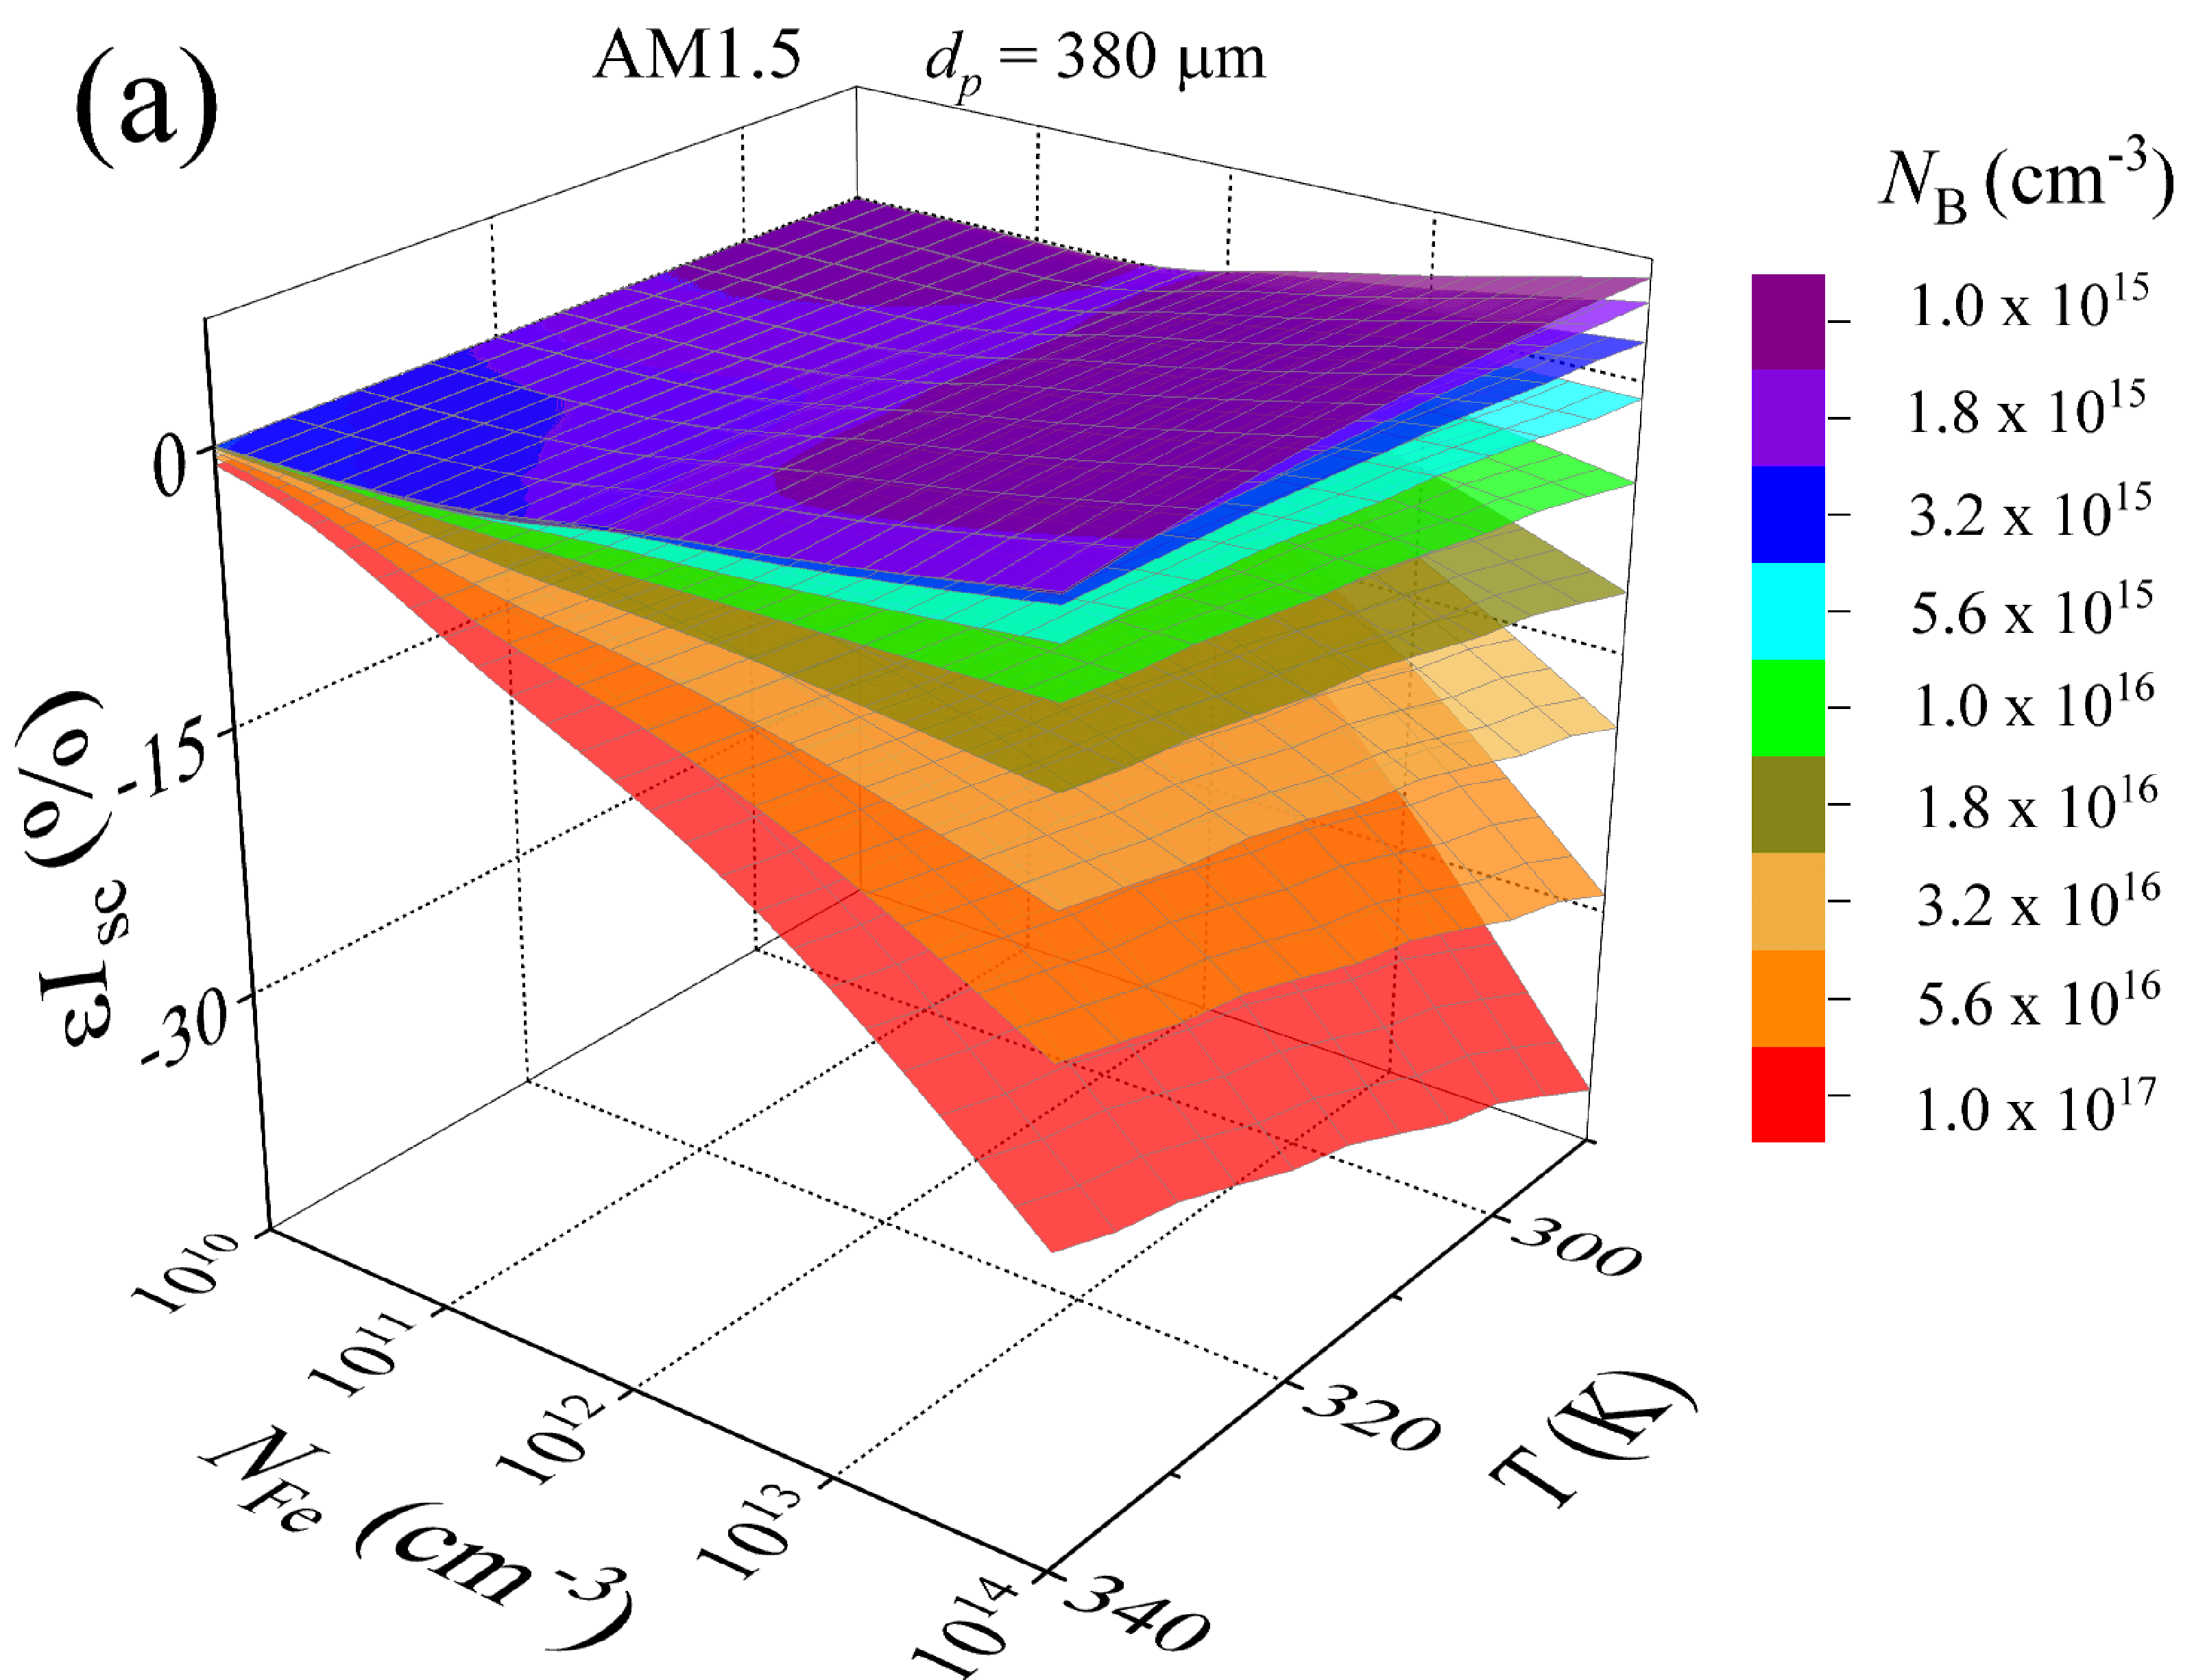
\includegraphics[width=0.49\linewidth]{Fig3a.png}
     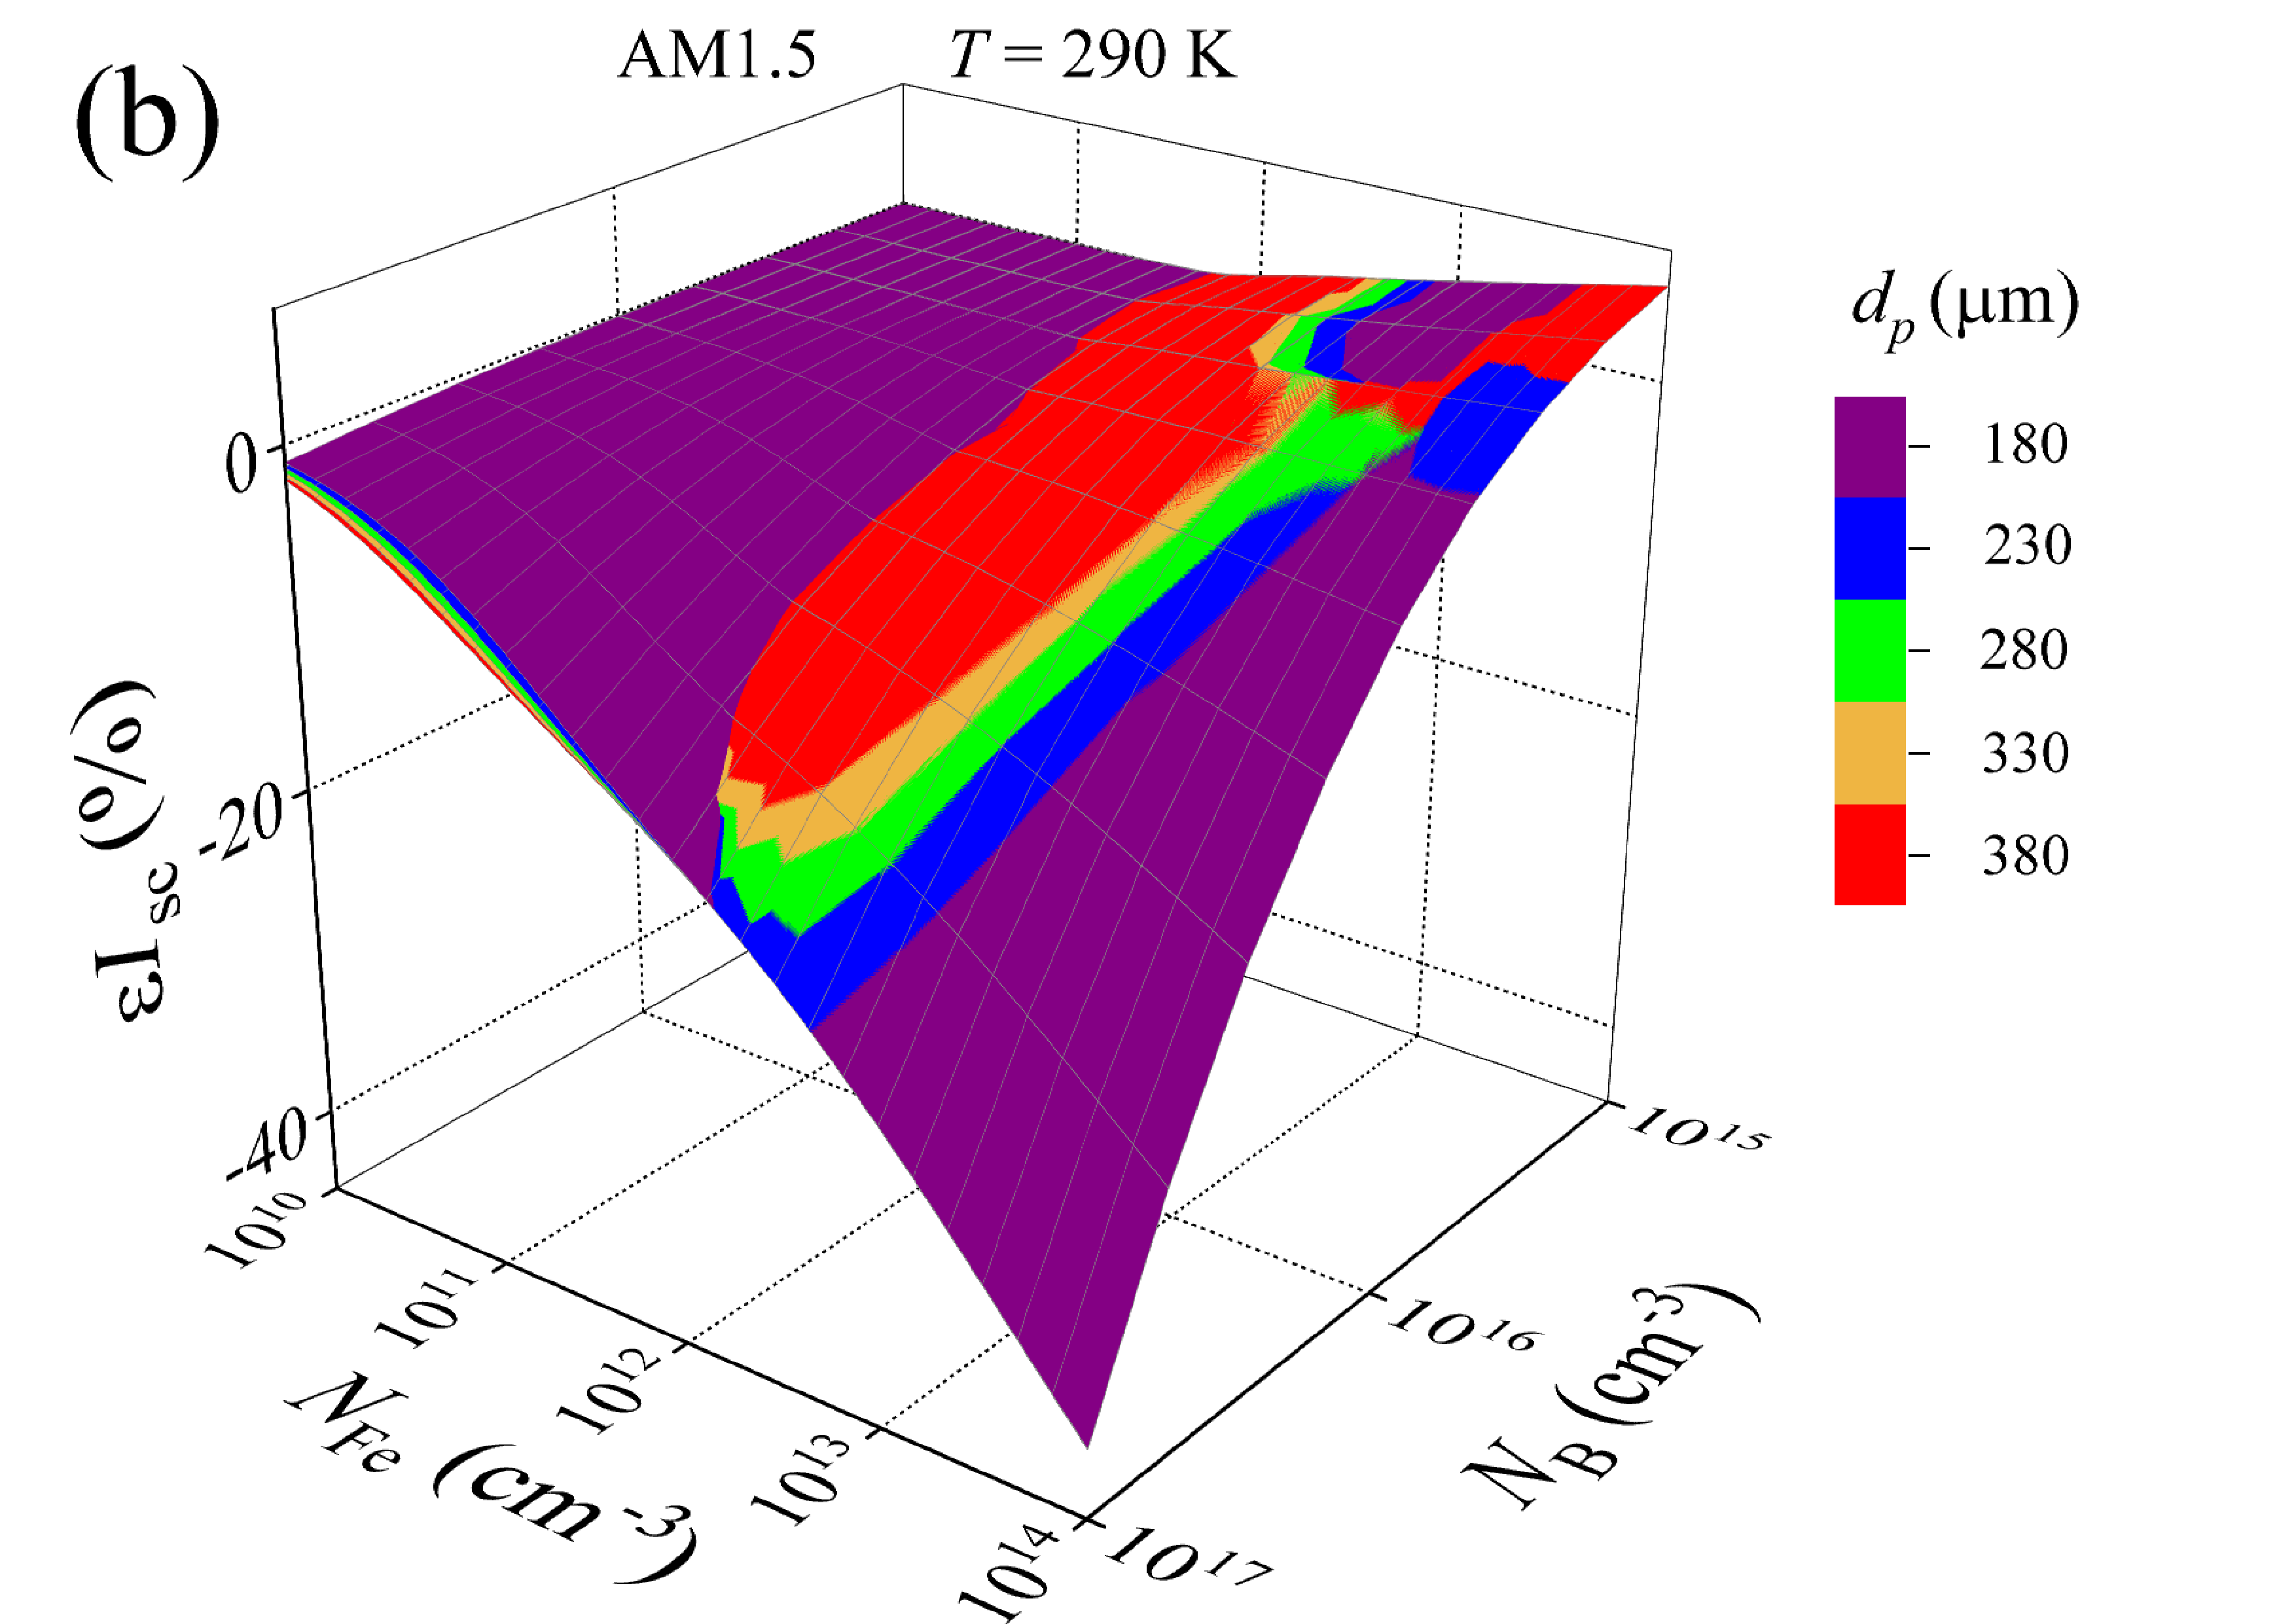
\includegraphics[width=0.49\linewidth]{Fig3b.png}
     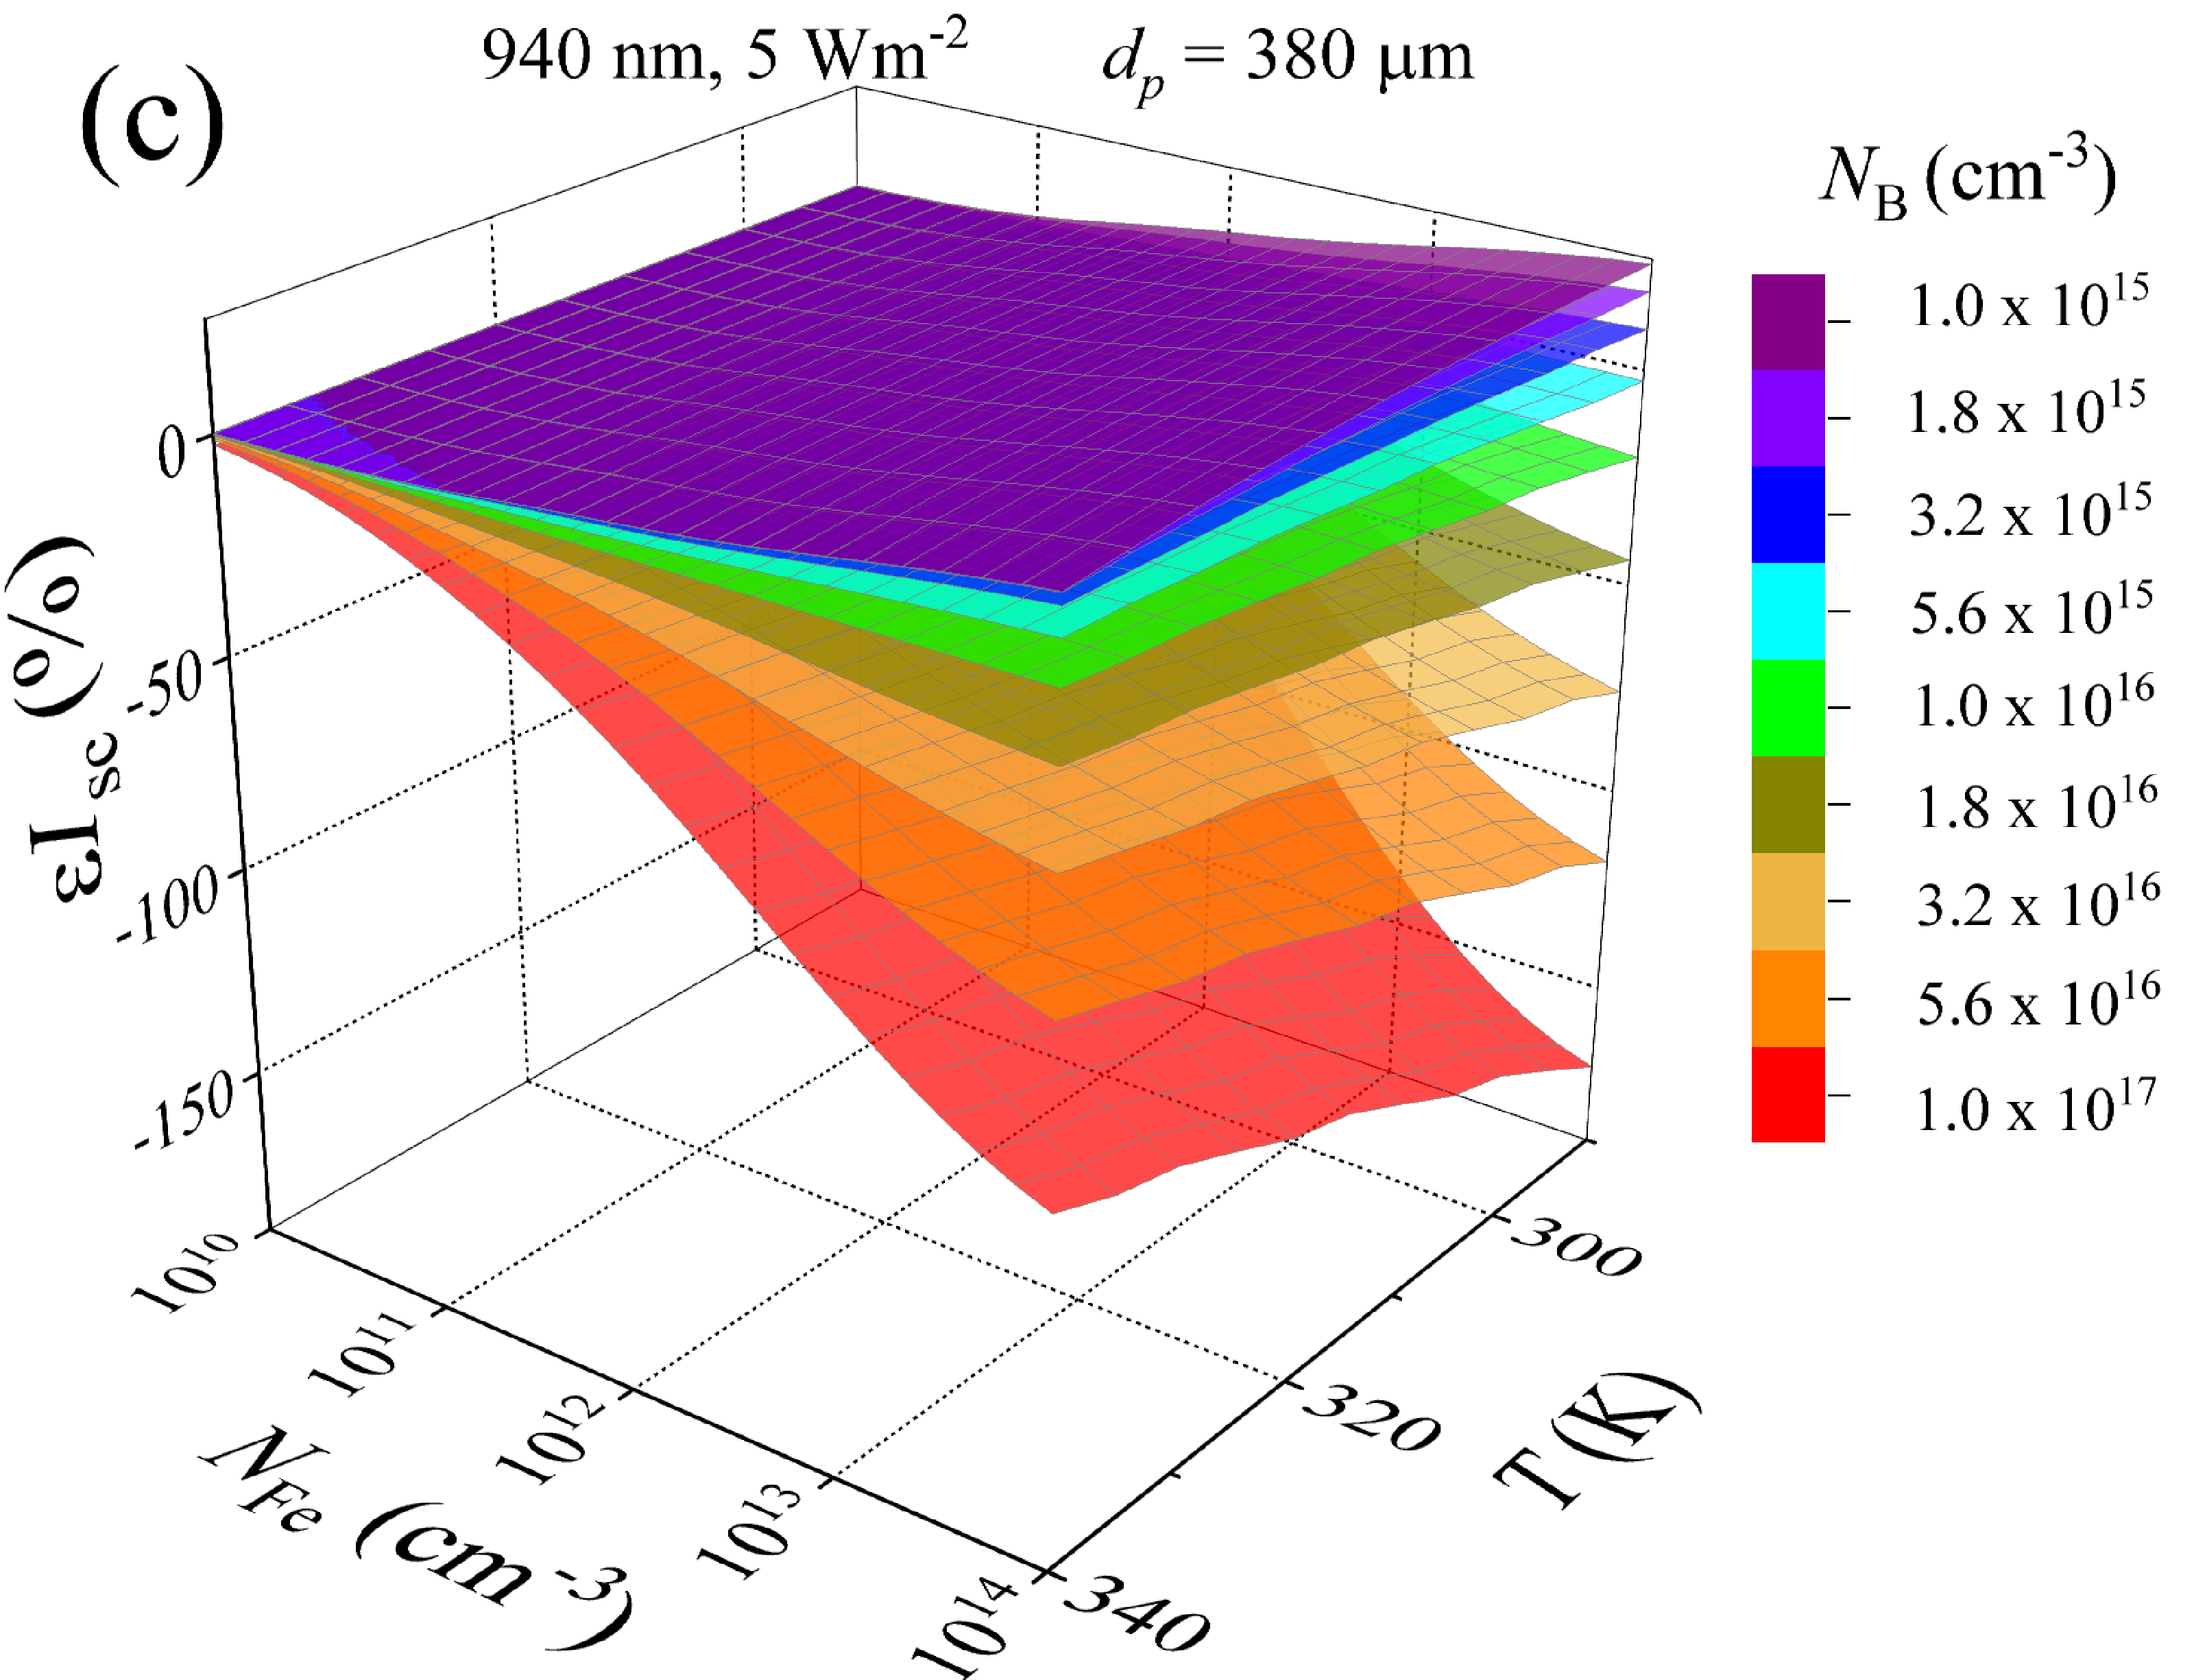
\includegraphics[width=0.49\linewidth]{Fig3c.png}
     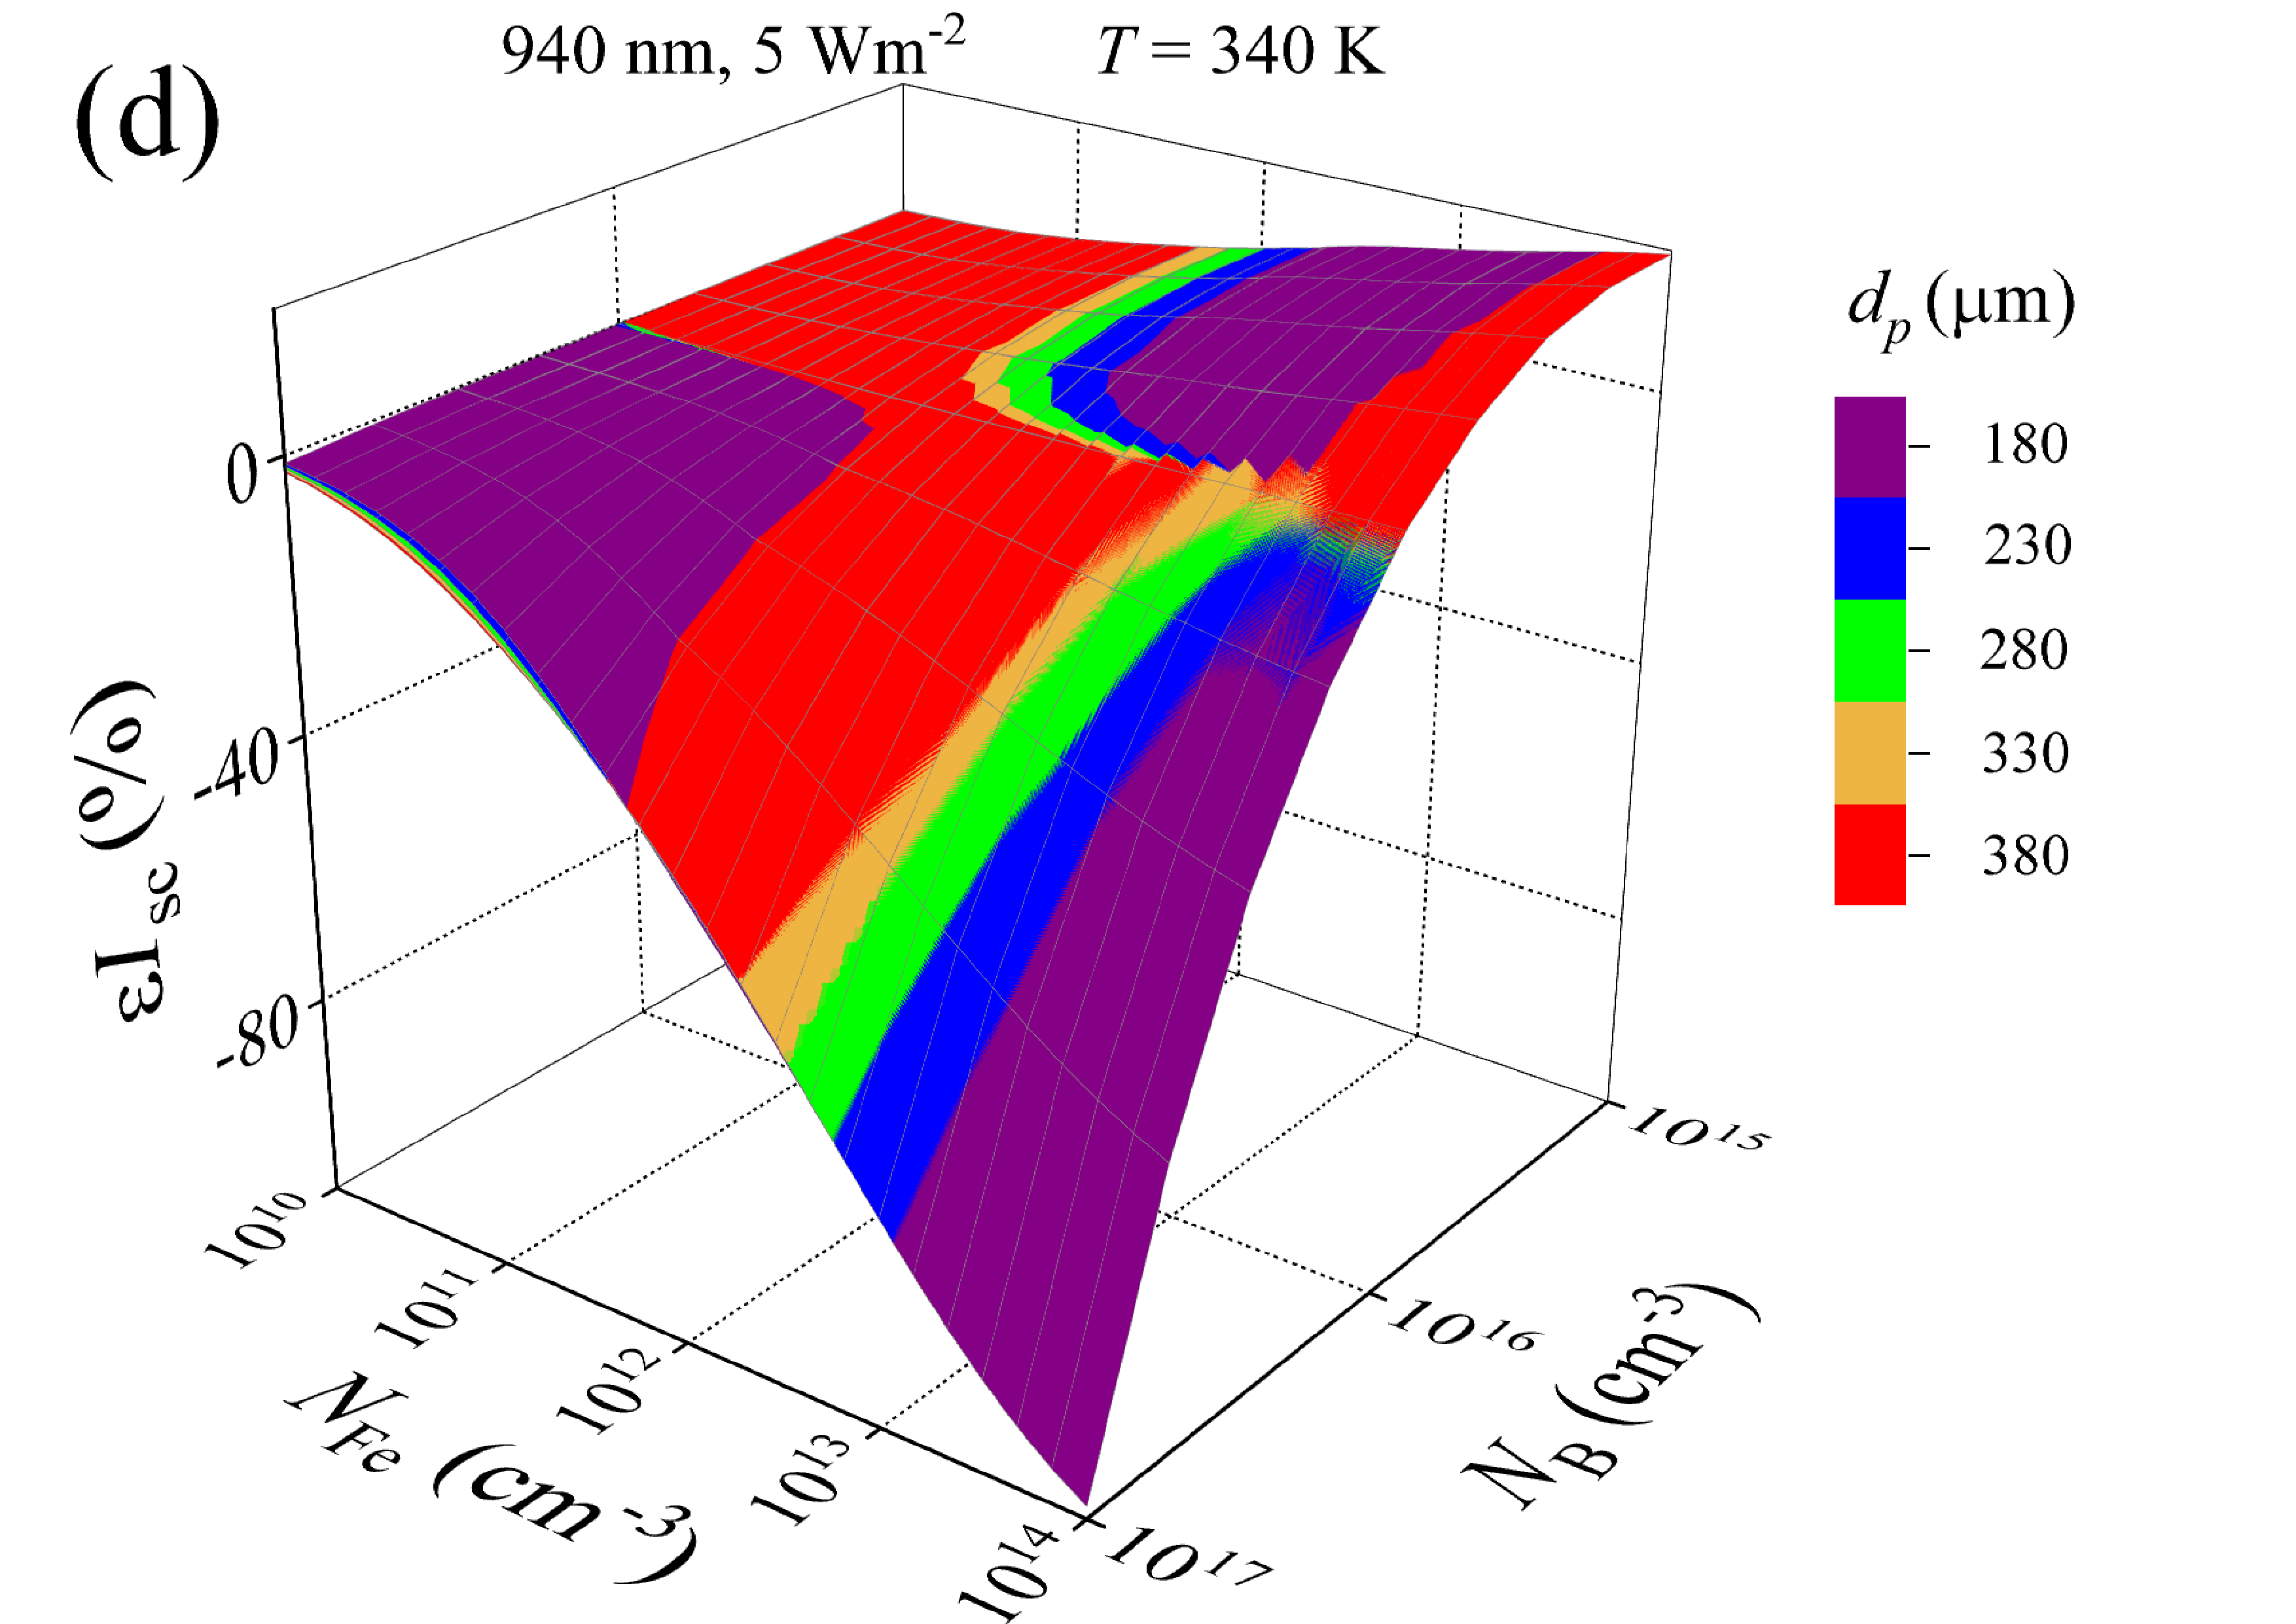
\includegraphics[width=0.49\linewidth]{Fig3d.png}
	  \caption{Relative changes in short-circuit current caused by a complete
       dissociation of Fe$_i$B$_s$ pairs as a function of
       iron concentration and
       temperature (panels a and c) or doping level (b, d).
       Illumination: AM1.5 (a, b), 940~nm 5~Wm$^{-2}$ (c, d).
       $T$, K: 290 (b), 340 (d).
       Different surfaces correspond to different doping levels (a, c) and base depths (b, d).
}\label{fig3}
\end{figure}


\begin{figure}
	\centering
     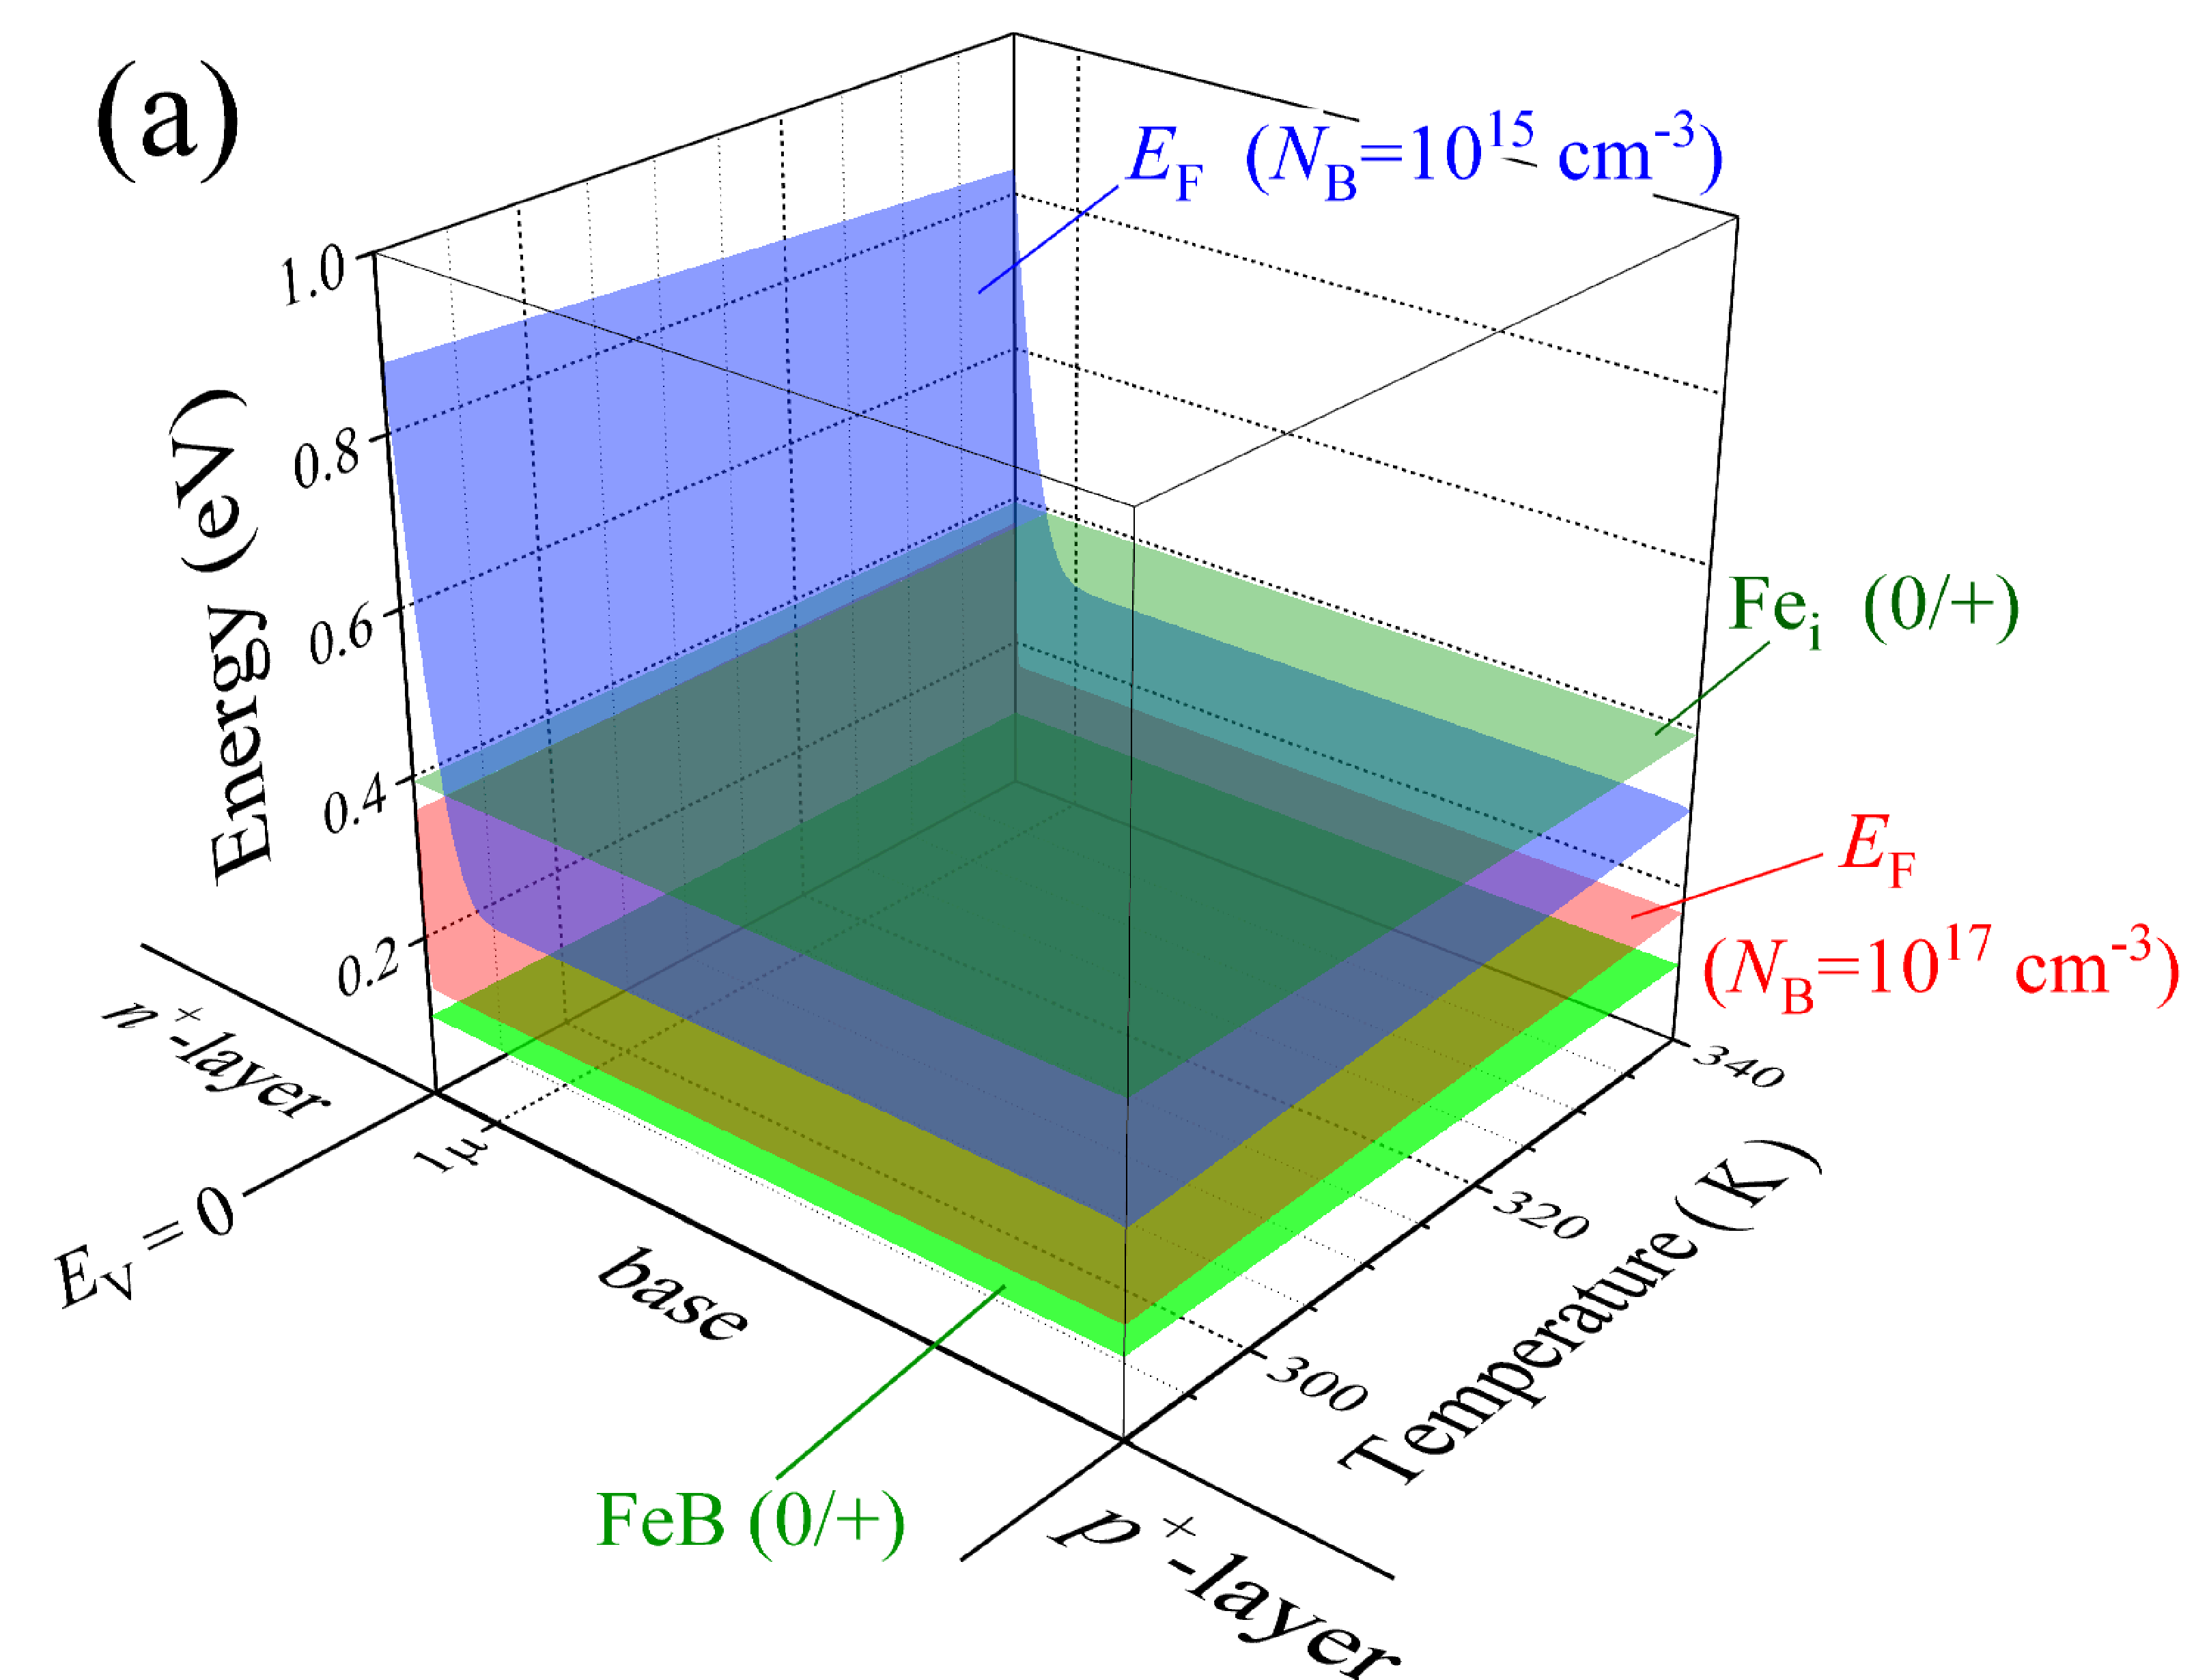
\includegraphics[width=0.49\linewidth]{Fig4a.png}
     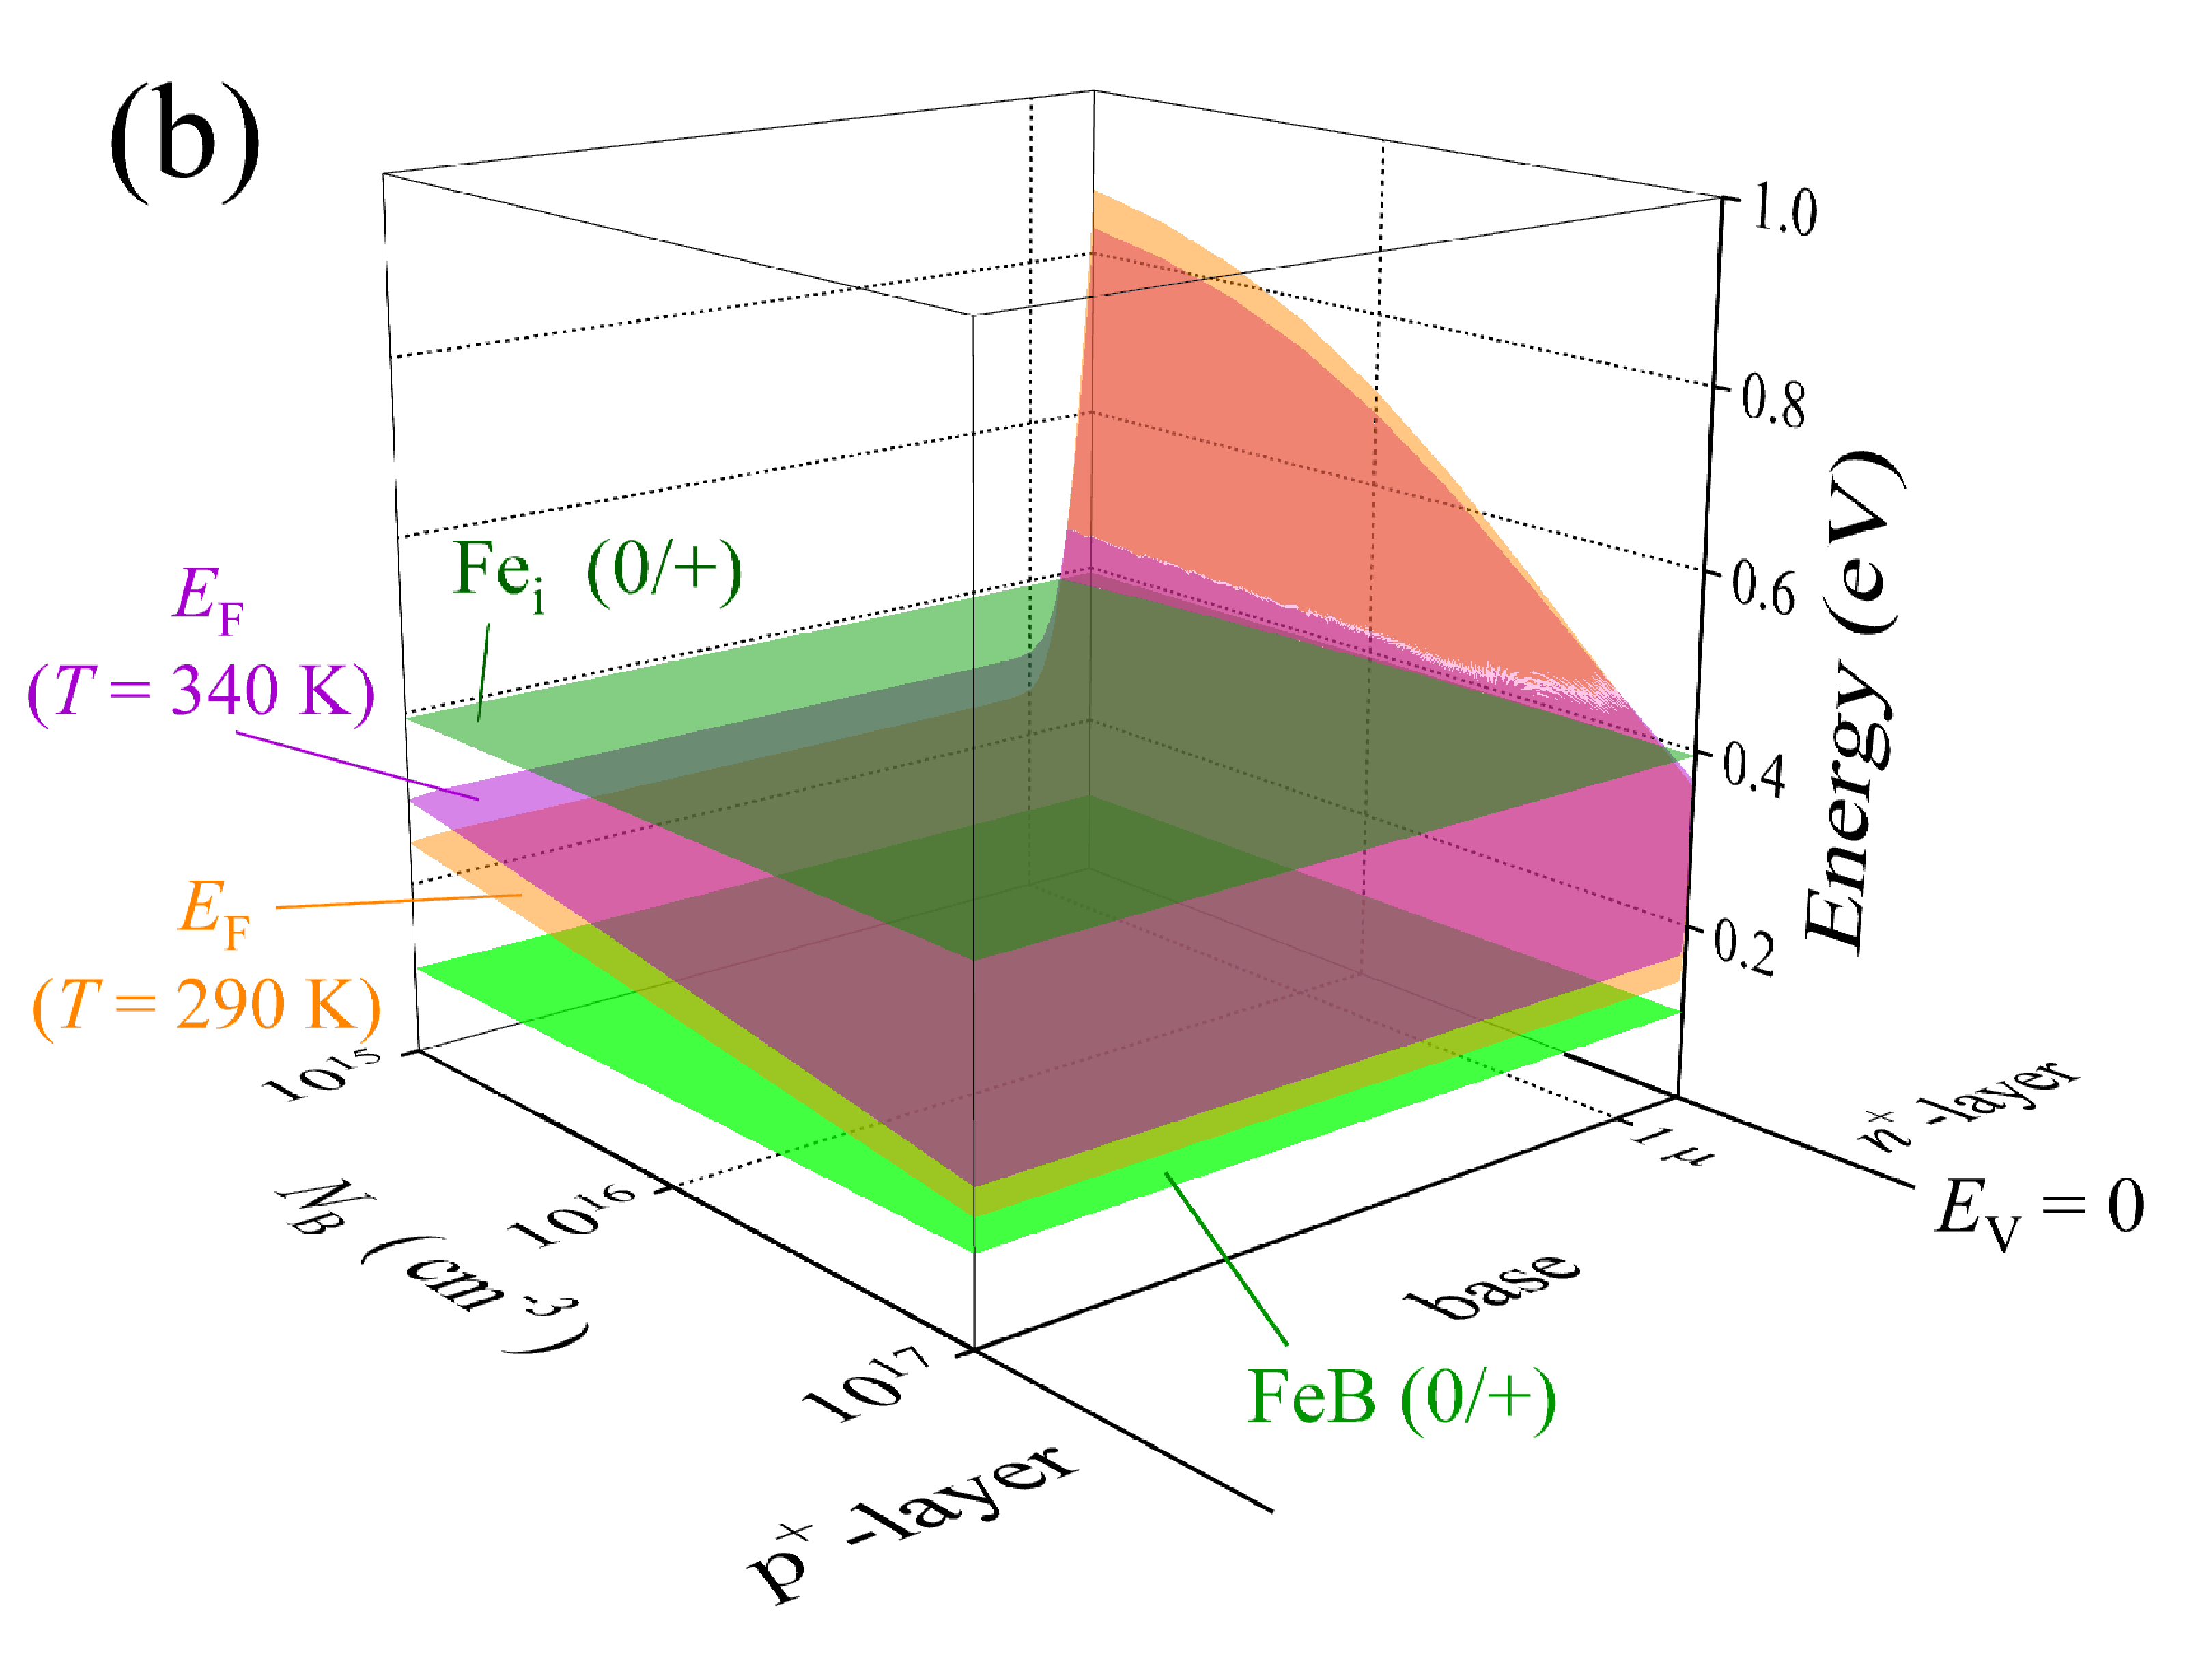
\includegraphics[width=0.49\linewidth]{Fig4b.png}
	  \caption{The location of the Fermi level in the base of the $n^+$-$p$-$p^+$ structure
       as a function of temperature for $N_\mathrm{B}=10^{15}$ and $10^{17}$~cm$^{-3}$ (a),
       and as a function of the doping level for $T=290$ and 340~K (b).
       The zero energy value corresponds to the top of the valence band.
       Also shown are the locations of the donor (0/+) levels for the FeB pair (green surfaces)
       and the interstitial iron atom Fe$_i$ (olive surfaces) and acceptor (-/0) level for FeB pair (brown surfaces).
}\label{fig4}
\end{figure}


\begin{figure}
	\centering
     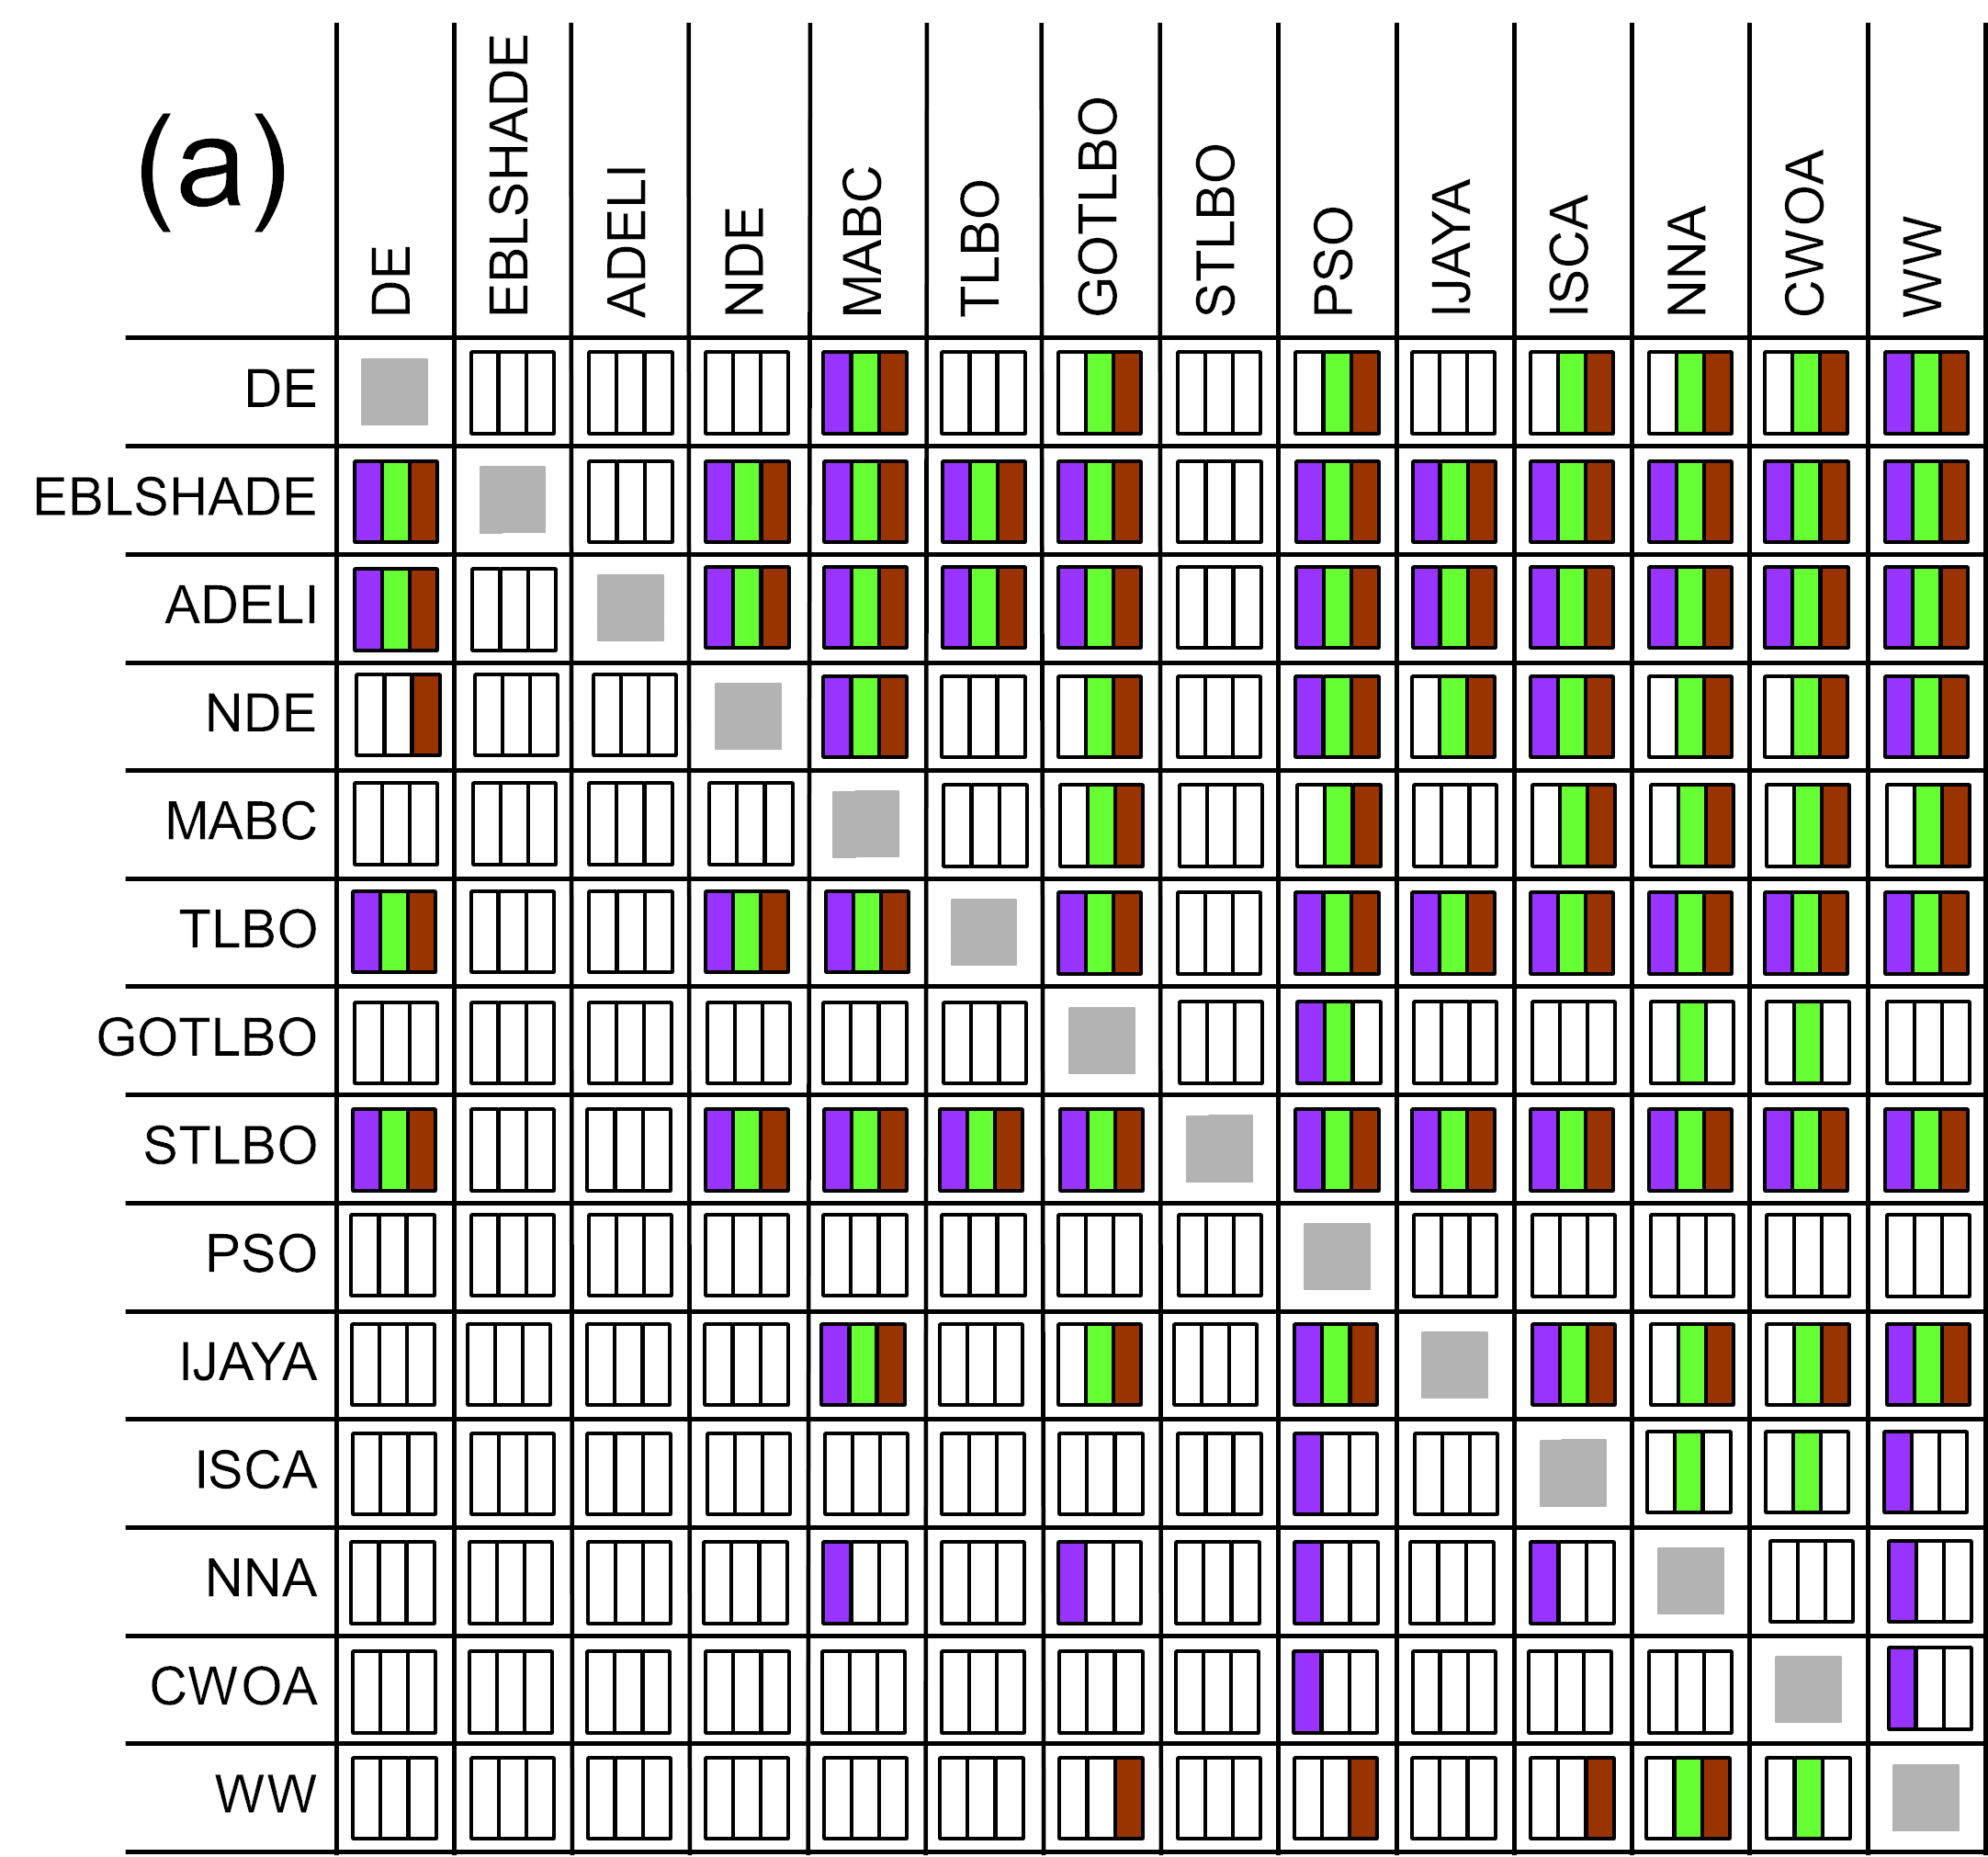
\includegraphics[width=0.4\linewidth]{Fig5a.png}
     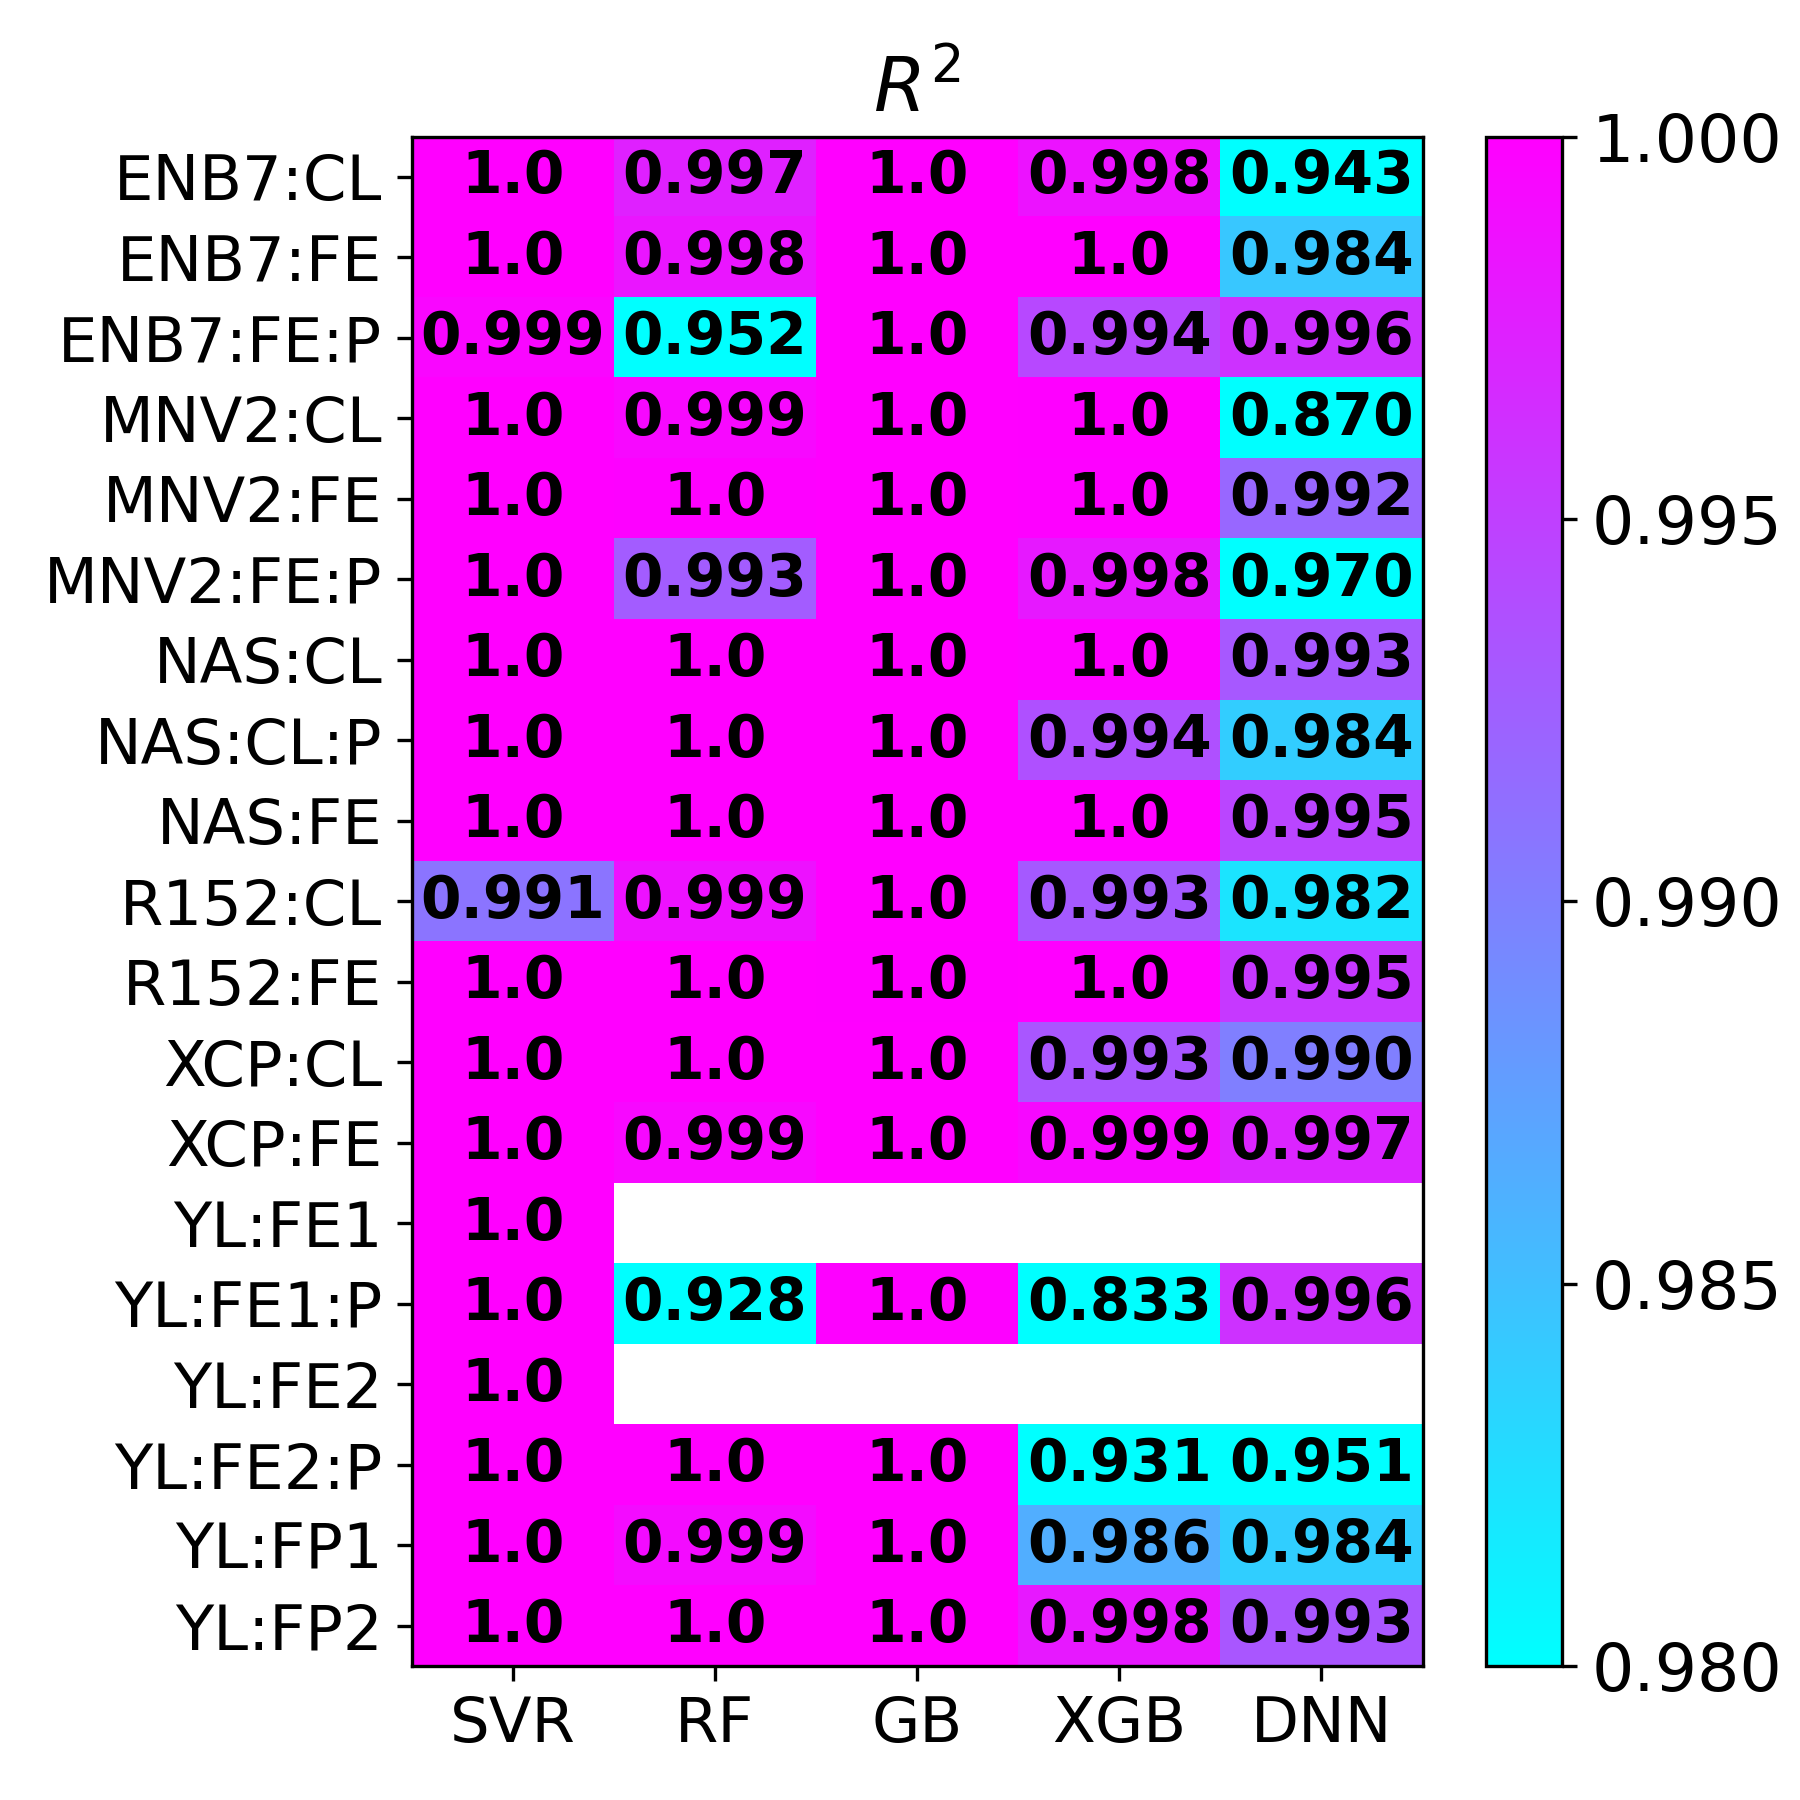
\includegraphics[width=0.4\linewidth]{Fig5b.png}
	  \caption{Relative changes in short-circuit current caused by a complete
       dissociation of Fe$_i$B$_s$ pairs as a function of iron concentration (a) and
       temperature (b) for SSC with $d_p=380$~$\mu$m and $N_\mathrm{B}=1.36\times10^{15}$~cm$^{-3}$
       in the case of monochromatic (940~nm) illumination.
       The marks are the experimental results (divided by factor $C_{cor}=1.4$), the lines are the simulation results.
       $W_\mathrm{ill}$, Wm$^{-2}$: 5 (marks and solid lines), 10 (dotted lines).
       Different lines and marks correspond to different temperatures (a) or $N_\mathrm{Fe}$ values (b) --- see legends.
}\label{fig5}
\end{figure}

\subsection{Open-circuit voltage}

Figure~\ref{fig7} presents the characteristic simulation results of open-circuit voltage changes due to the dissociation of FeB pairs. Figures S7-S12 in the Supplementary Material show additional $\varepsilon V_\mathrm{OC}$ dependencies. Notably, the changes in $V_\mathrm{OC}$ are almost an order of magnitude smaller than the values observed for $I_\mathrm{SC}$. Moreover, there are notable differences in the behavior of open-circuit voltage changes as a function of iron concentration at low ($N_\mathrm{B}<2\times10^{16}$~cm$^{-3}$) base doping levels under monochromatic and AM1.5 illumination. Under solar illumination, $\varepsilon V_\mathrm{OC}$ values are negative, and the $\varepsilon V_\mathrm{OC}$$\left(N_\mathrm{Fe}\right)$ dependency is non-monotonic (Figures~\ref{fig6}a,~\ref{fig6}b). The base thickness significantly affects the iron concentration at which the minimum $\varepsilon V_\mathrm{OC}$ value occurs (Figure~\ref{fig6}a). When illuminated with photons of 940~nm wavelength, $\varepsilon V_\mathrm{OC}$ values are positive and increase monotonically with increasing iron concentration. With increasing boron concentration, the behavior of $\varepsilon V_\mathrm{OC}$$\left(N_\mathrm{Fe}\right)$ becomes similar regardless of the type of illumination: the relative changes in open-circuit voltage during the restructuring of iron-containing defects are negative and increase monotonically in absolute value with increasing $N_\mathrm{Fe}$ and $N_\mathrm{B}$. Furthermore, the changes in $V_\mathrm{OC}$ are more significant under monochromatic illumination, as observed for the short-circuit current.

The effect of temperature on $\varepsilon V_\mathrm{OC}$ also depends on the base doping level: as $N_\mathrm{B}$ increases, the temperature coefficient of $\varepsilon V_\mathrm{OC}$ gradually changes from positive to negative, and this trend is characteristic for both AM1.5 and 940~nm illumination - see Figures S9,~\ref{fig6}a,~\ref{fig6}b. The influence of $d_p$ on the open-circuit voltage changes is slightly greater than that observed for $\varepsilon I_\mathrm{SC}$; however, base thickness is not a determining factor for $\varepsilon V_\mathrm{OC}$ and mainly affects low doping levels and temperatures - see Figures S9, S11, and S12. Another difference in the behavior of $\varepsilon V_\mathrm{OC}$ compared to $\varepsilon I_\mathrm{SC}$ is its dependence on the monochromatic illumination intensity: for $W_\mathrm{ill}$ = 10~Wm$^{-2}$ the changes in the open-circuit voltage are smaller, the differences increase with decreasing iron concentration and are weakly dependent on temperature.

Understanding the features of $\varepsilon V_\mathrm{OC}$ requires recalling that the open-circuit voltage depends not only on the photocurrent but also on the saturation current $I_\mathrm{0}$ and the ideality factor, which in turn are determined by the state of the defect subsystem and other parameters that varied during the simulation also determine \cite{Olikh2019SM,YangHandbookPVSi}. For a simplified single-diode model \cite{YangHandbookPVSi}:
\begin{equation}
\label{eq5}
     V_\mathrm{OC} = nkT\left[ {\ln\left( {\frac{I_\mathrm{ph}}{I_\mathrm{0}}} \right)+1} \right].
\end{equation}

Similar to the photocurrent, we can express $I_\mathrm{0}$ as the sum of the currents from the base and the emitter \cite{Markvart}:
\begin{equation}
\label{eq6}
     I_\mathrm{0} = I_\mathrm{0,e}+I_\mathrm{0,b},
\end{equation}
we can then express the second term as \cite{Goetzberger1998}:
\begin{equation}
\label{eq7}
     I_\mathrm{0,b}=\frac{qn_\mathrm{i}D_\mathrm{n}}{N_\mathrm{B}L_\mathrm{n}}\cdot\frac{\frac{D_\mathrm{n}}{SL_\mathrm{n}}\sinh\left( \frac{d_p}{L_\mathrm{n}} \right)+\cosh\left( \frac{d_p}{L_\mathrm{n}} \right)}{\sinh\left( \frac{d_p}{L_\mathrm{n}} \right)+\frac{D_\mathrm{n}}{SL_\mathrm{n}}\cosh\left( \frac{d_p}{L_\mathrm{n}} \right)},
\end{equation}
where $n_\mathrm{i}$ is the carrier concentration in the intrinsic semiconductor. The last formula explains the observed dependence of $\varepsilon V_\mathrm{OC}$ on the base thickness.

Previous studies \cite{Olikh2022PPV,Olikh2019SM} demonstrate that changes in the ideality factor during restructuring Fe$_i$B$_\mathrm{Si}$ $\rightleftharpoons$ Fe$_i$ + B$_\mathrm{Si}$ do not exceed a few percent. This slight variation and the logarithmic dependence of $V_\mathrm{OC}$ in equation (\ref{eq5}) account for the small absolute values of $\varepsilon V_\mathrm{OC}$.

Regarding the non-monotonicity of the dependence of $\varepsilon V_\mathrm{OC}$$\left(N_\mathrm{Fe}\right)$ (Fig.~\ref{fig6}b), Schmidt \cite{FeB:Schmidt}  attributes this effect to the much larger injection level in the cell base under open-circuit than under short-circuit conditions. Overall, the obtained data support this hypothesis: for monochromatic illumination with significantly lower intensity, the injection level is smaller and does not exceed the crossover point \cite{FeB:Schmidt} at any points on the $I$-$V$ curve, resulting in the absence of a minimum in the $\varepsilon V_\mathrm{OC}$$\left(N_\mathrm{Fe}\right)$ dependence.

The data presented in Fig.~\ref{fig7} allows for a comparison between the experimental and simulation results. Overall, the qualitative nature of the results in both cases coincides. However, to align the absolute values, it is necessary to use a correction factor that depends on the iron concentration: according to the obtained data, for low values of $N_\mathrm{Fe}$, $C_\mathrm{cor}$ < 1, and high values, $C_\mathrm{cor}$ > 1. Incidentally, Schubert et al. \cite{IronSC} observe this dependence of the correlation factor.

It can be believed \cite{YangHandbookPVSi} that the main effect of metals on the $V_\mathrm{OC}$ values can be determined by shunt formation. However, SCAPS does not allow the effect of shunt resistance to be taken into account, which, in our opinion, is the main reason for the differences between experimental and calculated values.

In summary, the relative changes in the open-circuit voltage due to the dissociation of FeB pairs are less convenient for estimating iron concentration than $\varepsilon I_\mathrm{SC}$. This is due to the smaller absolute values of $\varepsilon V_\mathrm{OC}$, the non-monotonic dependence $\varepsilon V_\mathrm{OC}$$\left(N_\mathrm{Fe}\right)$ under certain conditions, and the necessity to precisely control the intensity of the monochromatic illumination. At the same time, if $\varepsilon V_\mathrm{OC}$ is used as an additional parameter together with $\varepsilon I_\mathrm{SC}$, in the case of AM1.5 application, the accuracy of determining iron concentration for $N_\mathrm{Fe}<10^{11}$~cm$^{-3}$ and $N_\mathrm{B}=(1-5)\times10^{15}$~cm$^{-3}$ can be significantly improved: in this case, the dependence of $\varepsilon V_\mathrm{OC}$$\left(N_\mathrm{Fe}\right)$ is sufficiently sharp (Fig.~\ref{fig6}b), and we can resolve the ambiguity of associating a specific value of $\varepsilon V_\mathrm{OC}$ with iron concentration due to the monotonic behavior of $\varepsilon V_\mathrm{OC}$$\left(N_\mathrm{Fe}\right)$ in this range. Notably, the specified boron concentrations are most relevant to the most common real CSEs.


\begin{figure}
	\centering
     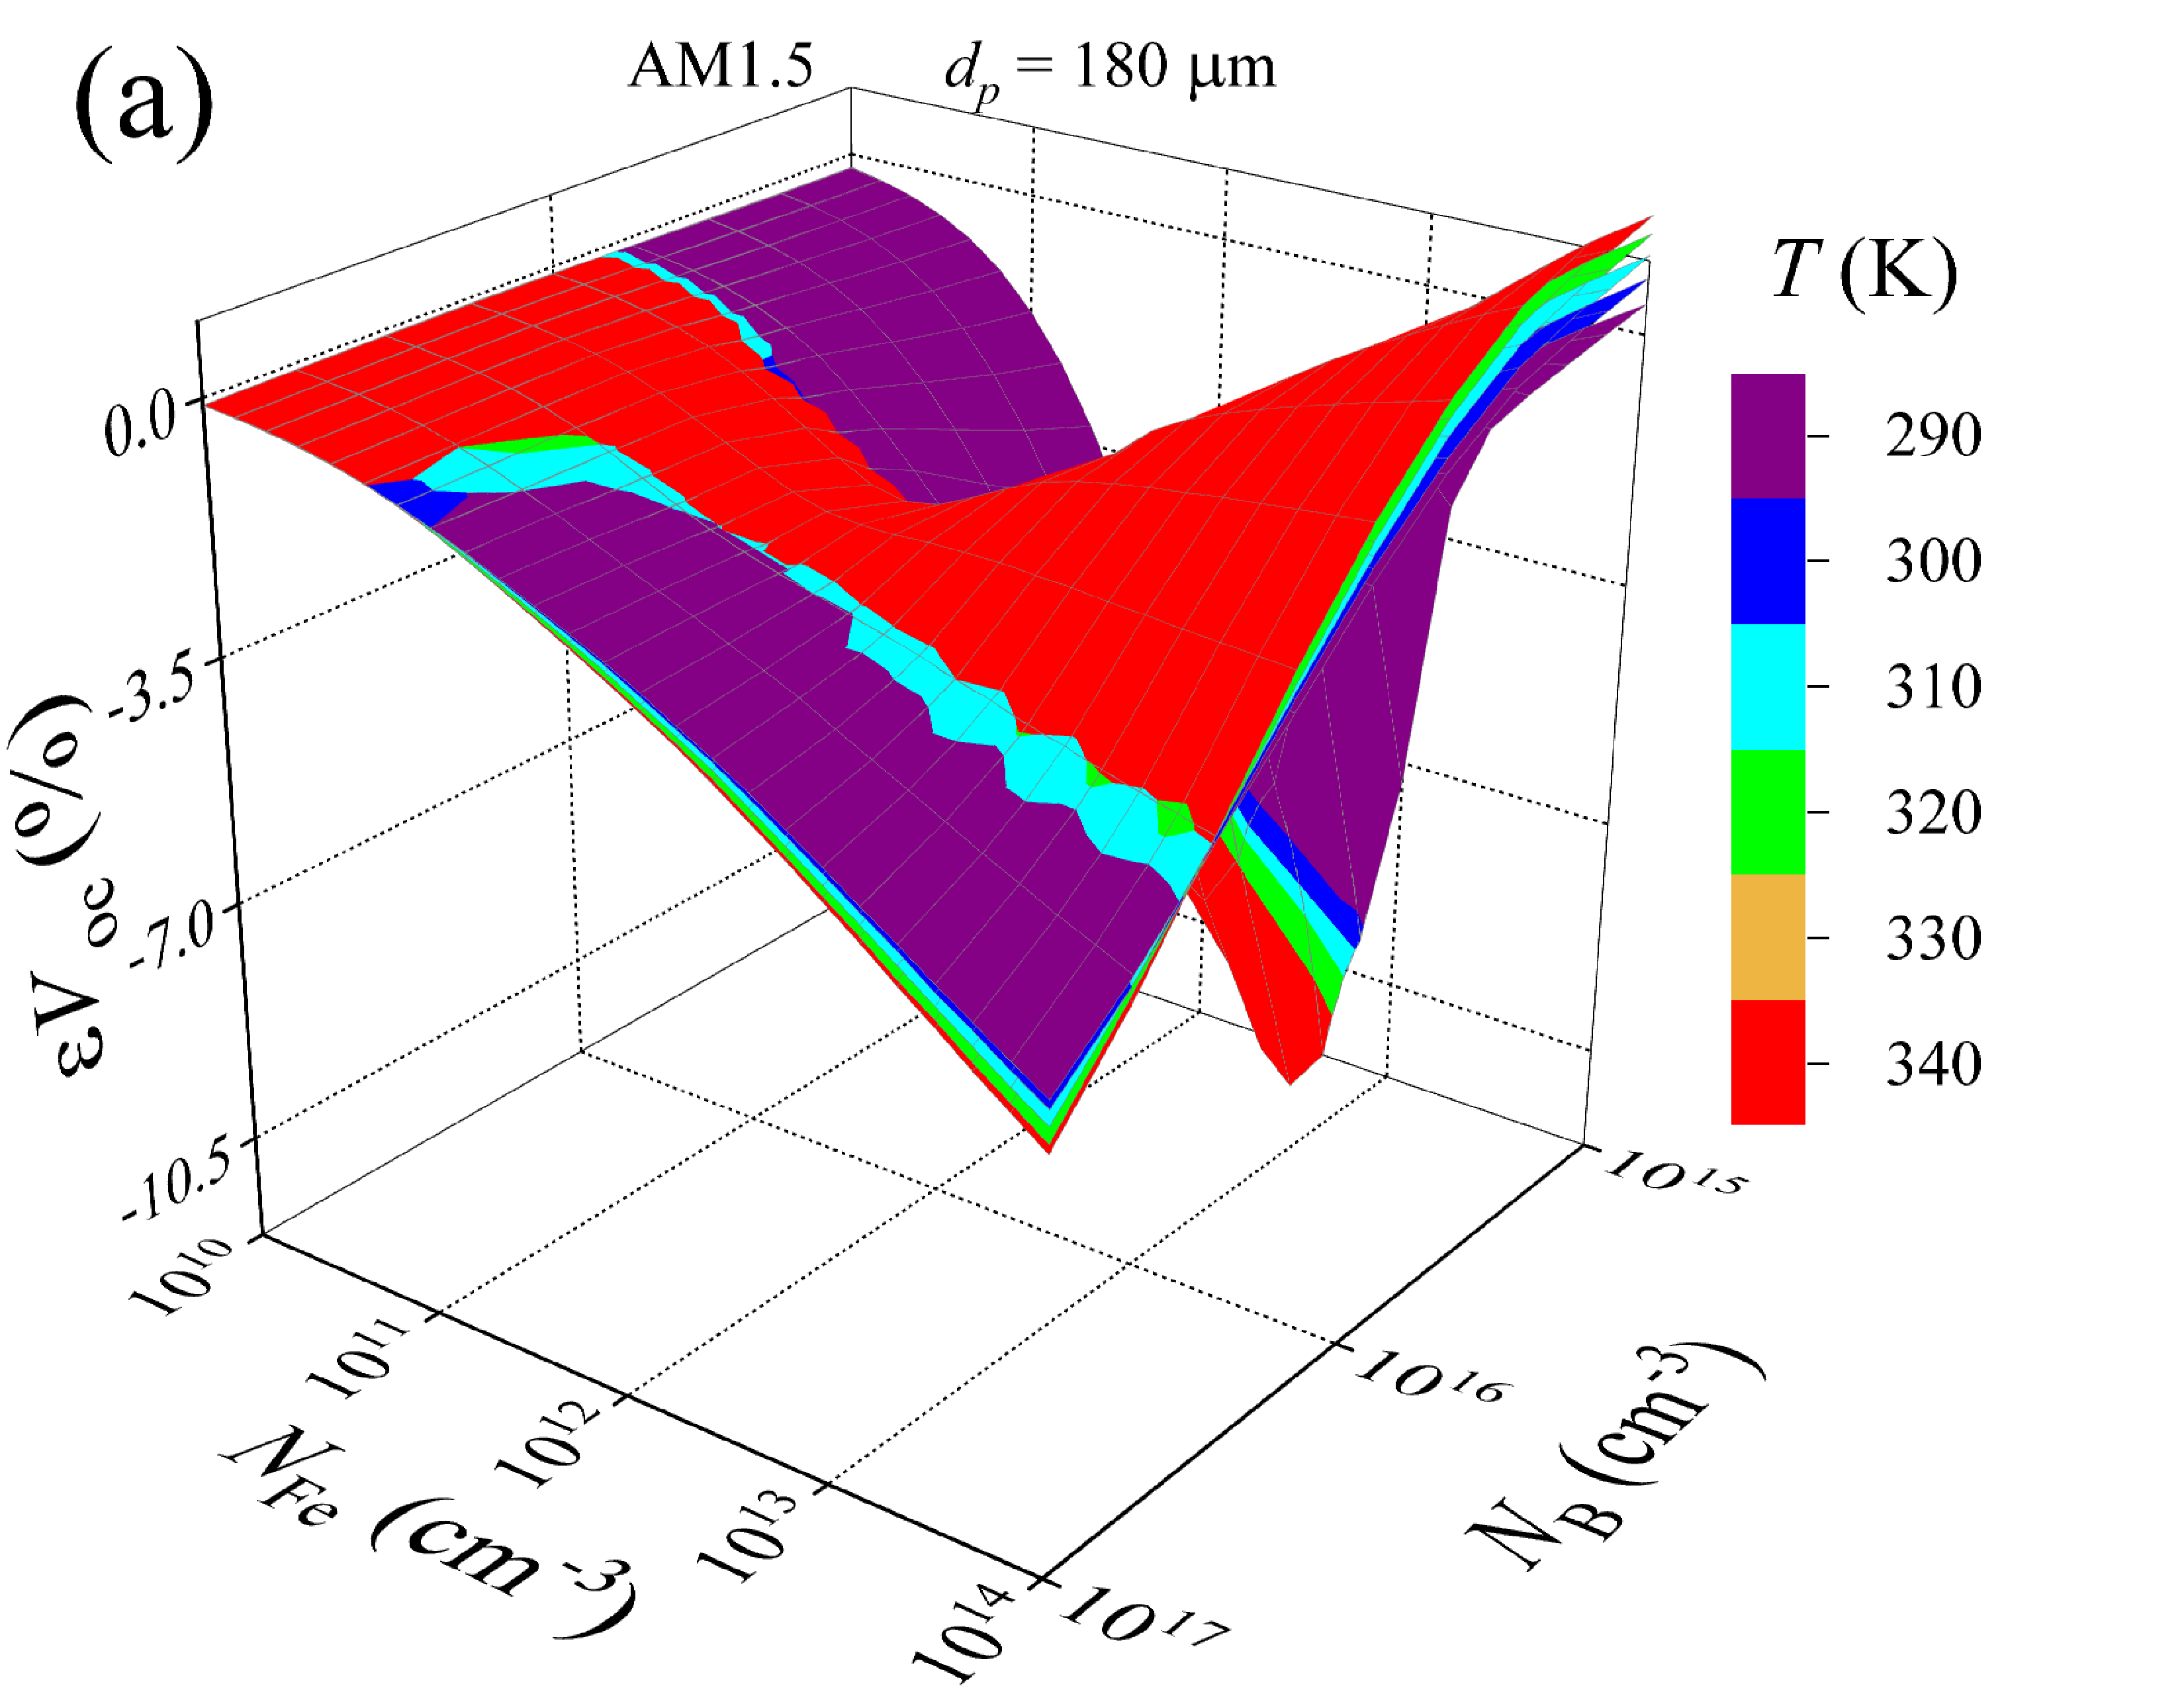
\includegraphics[width=0.49\linewidth]{Fig6a.png}
     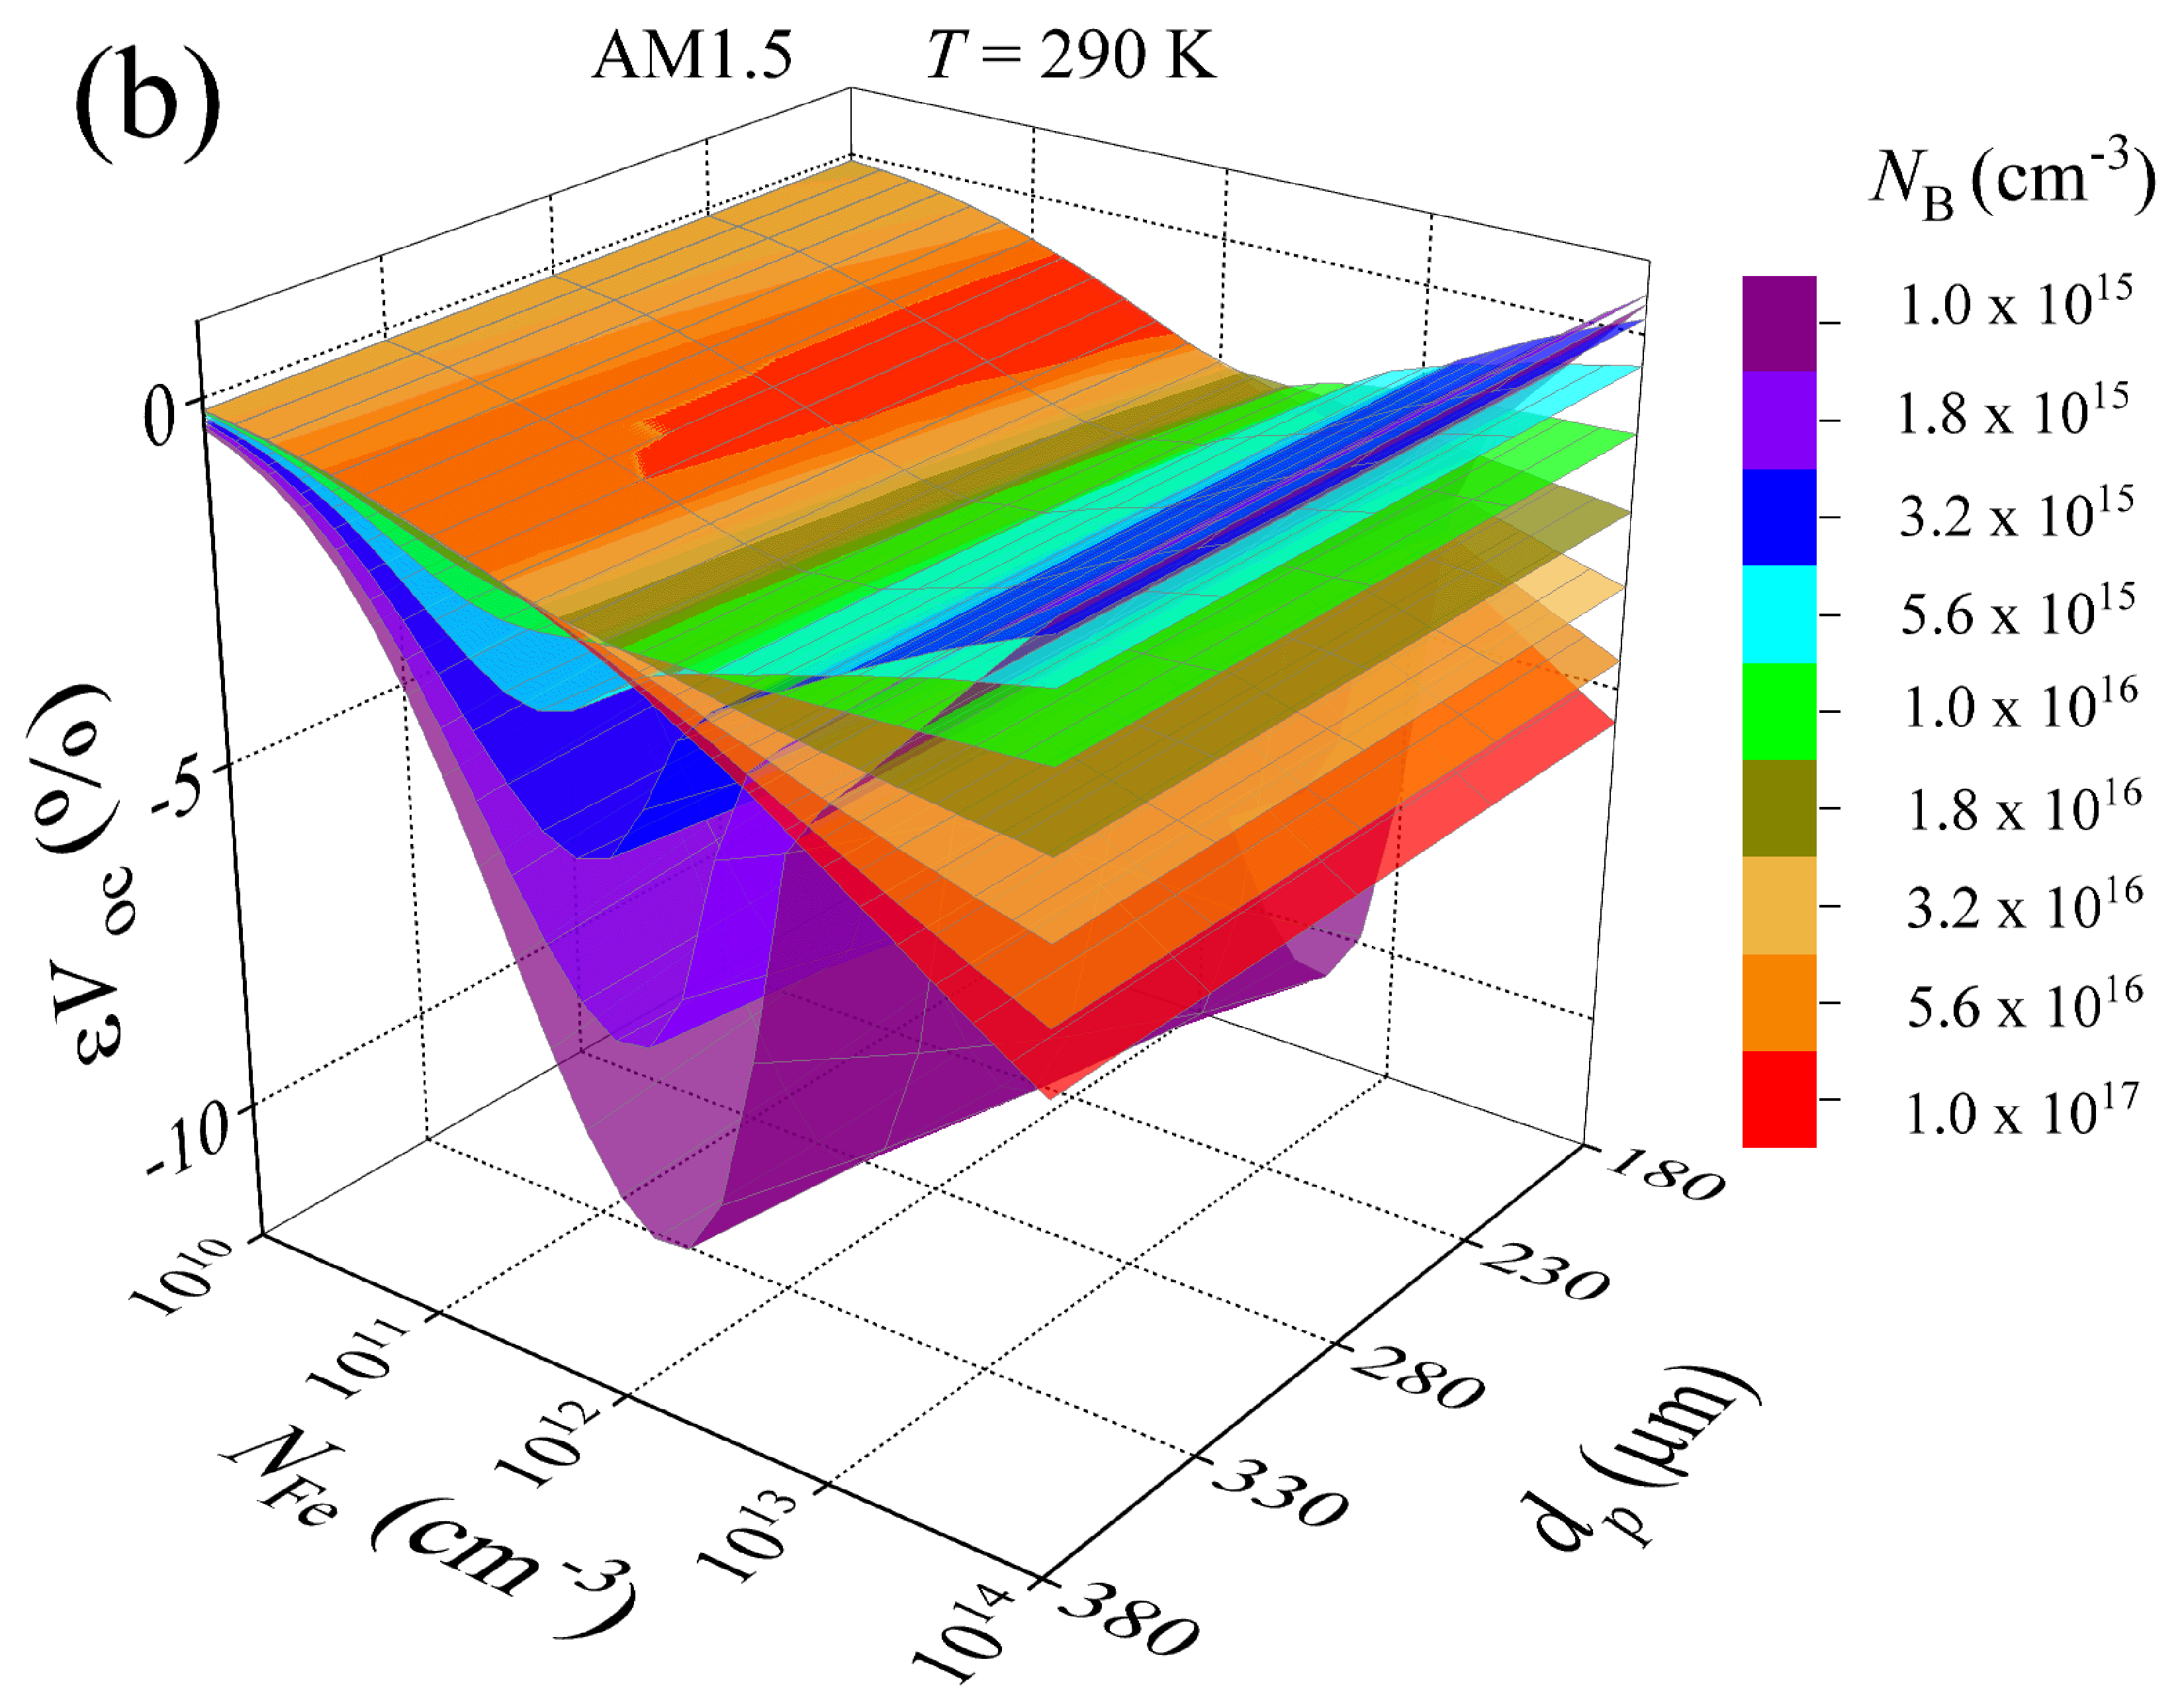
\includegraphics[width=0.49\linewidth]{Fig6b.png}
     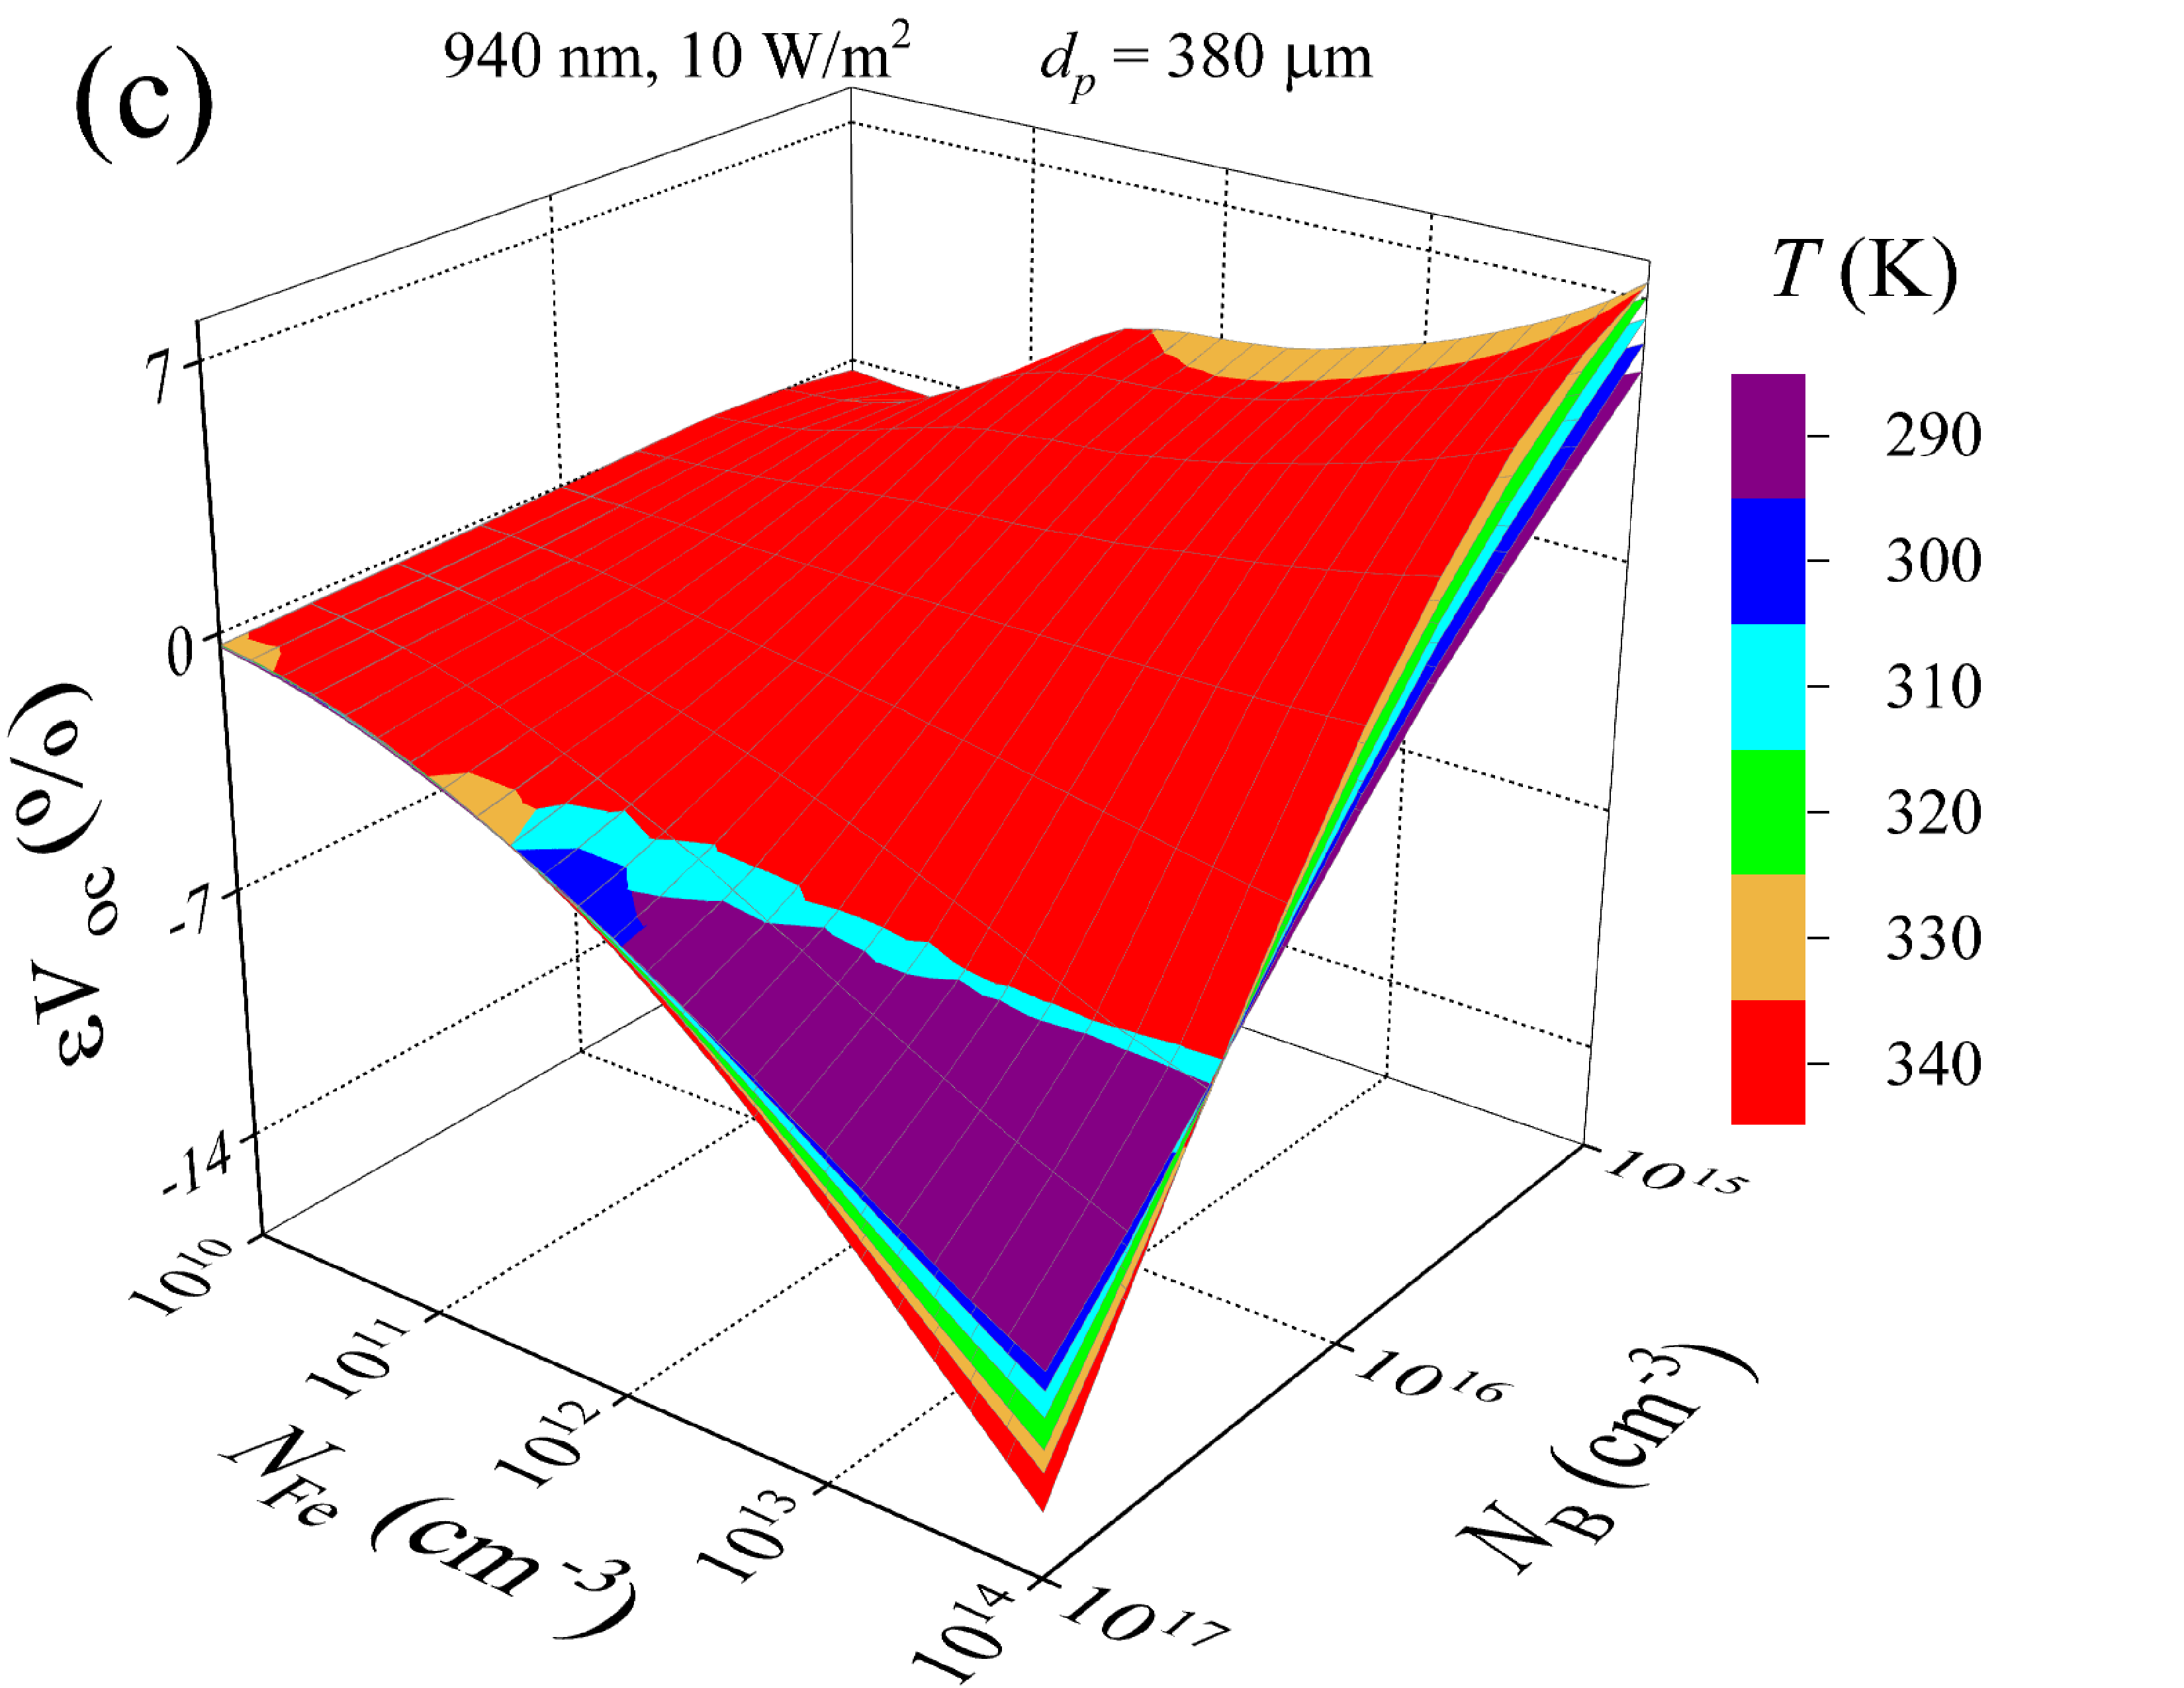
\includegraphics[width=0.49\linewidth]{Fig6c.png}
     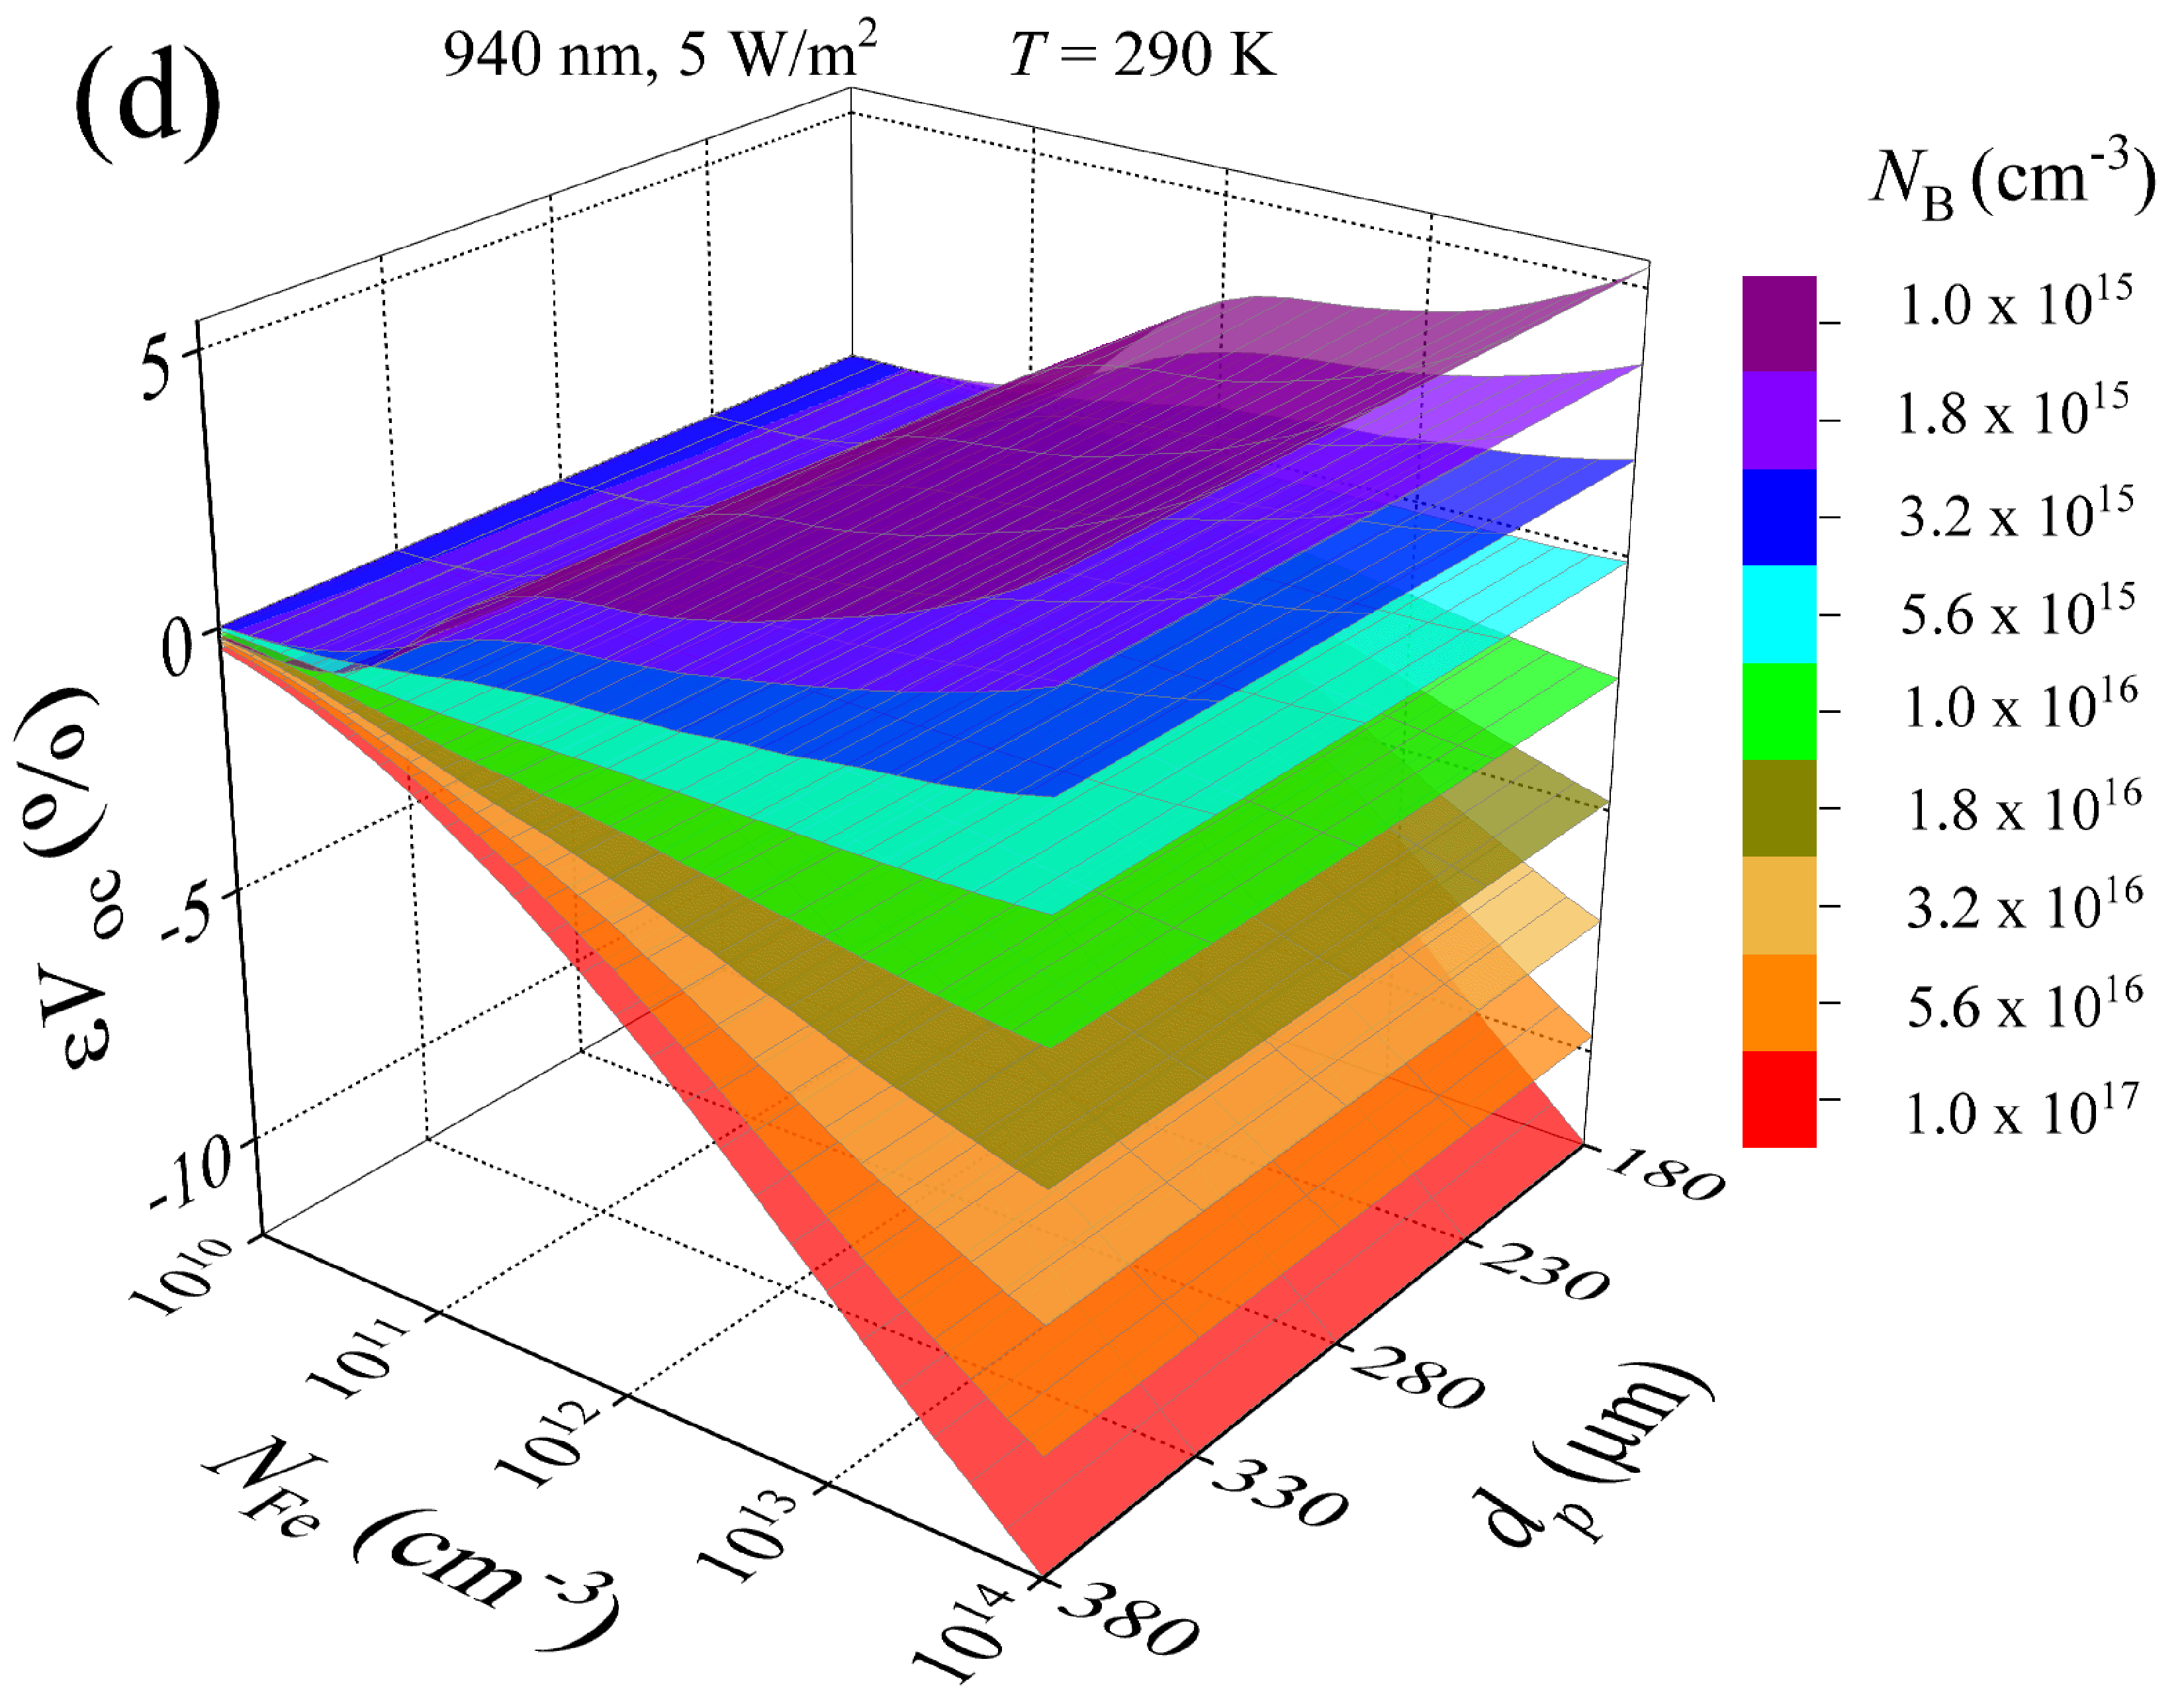
\includegraphics[width=0.49\linewidth]{Fig6d.png}
	  \caption{Relative changes in open-circuit voltage caused by a complete
       dissociation of Fe$_i$B$_s$ pairs as a function of
       iron concentration and
       doping level (panels a and c) or base depth (b, d).
       Illumination: AM1.5 (a, b), 940~nm 10~Wm$^{-2}$ (c),  940~nm 5~Wm$^{-2}$ (d).
       $T$, K: 290 (b, d).
       Different surfaces correspond to different temperatures (a, c) and doping levels (b, d).
}\label{fig6}
\end{figure}

\begin{figure}
	\centering
     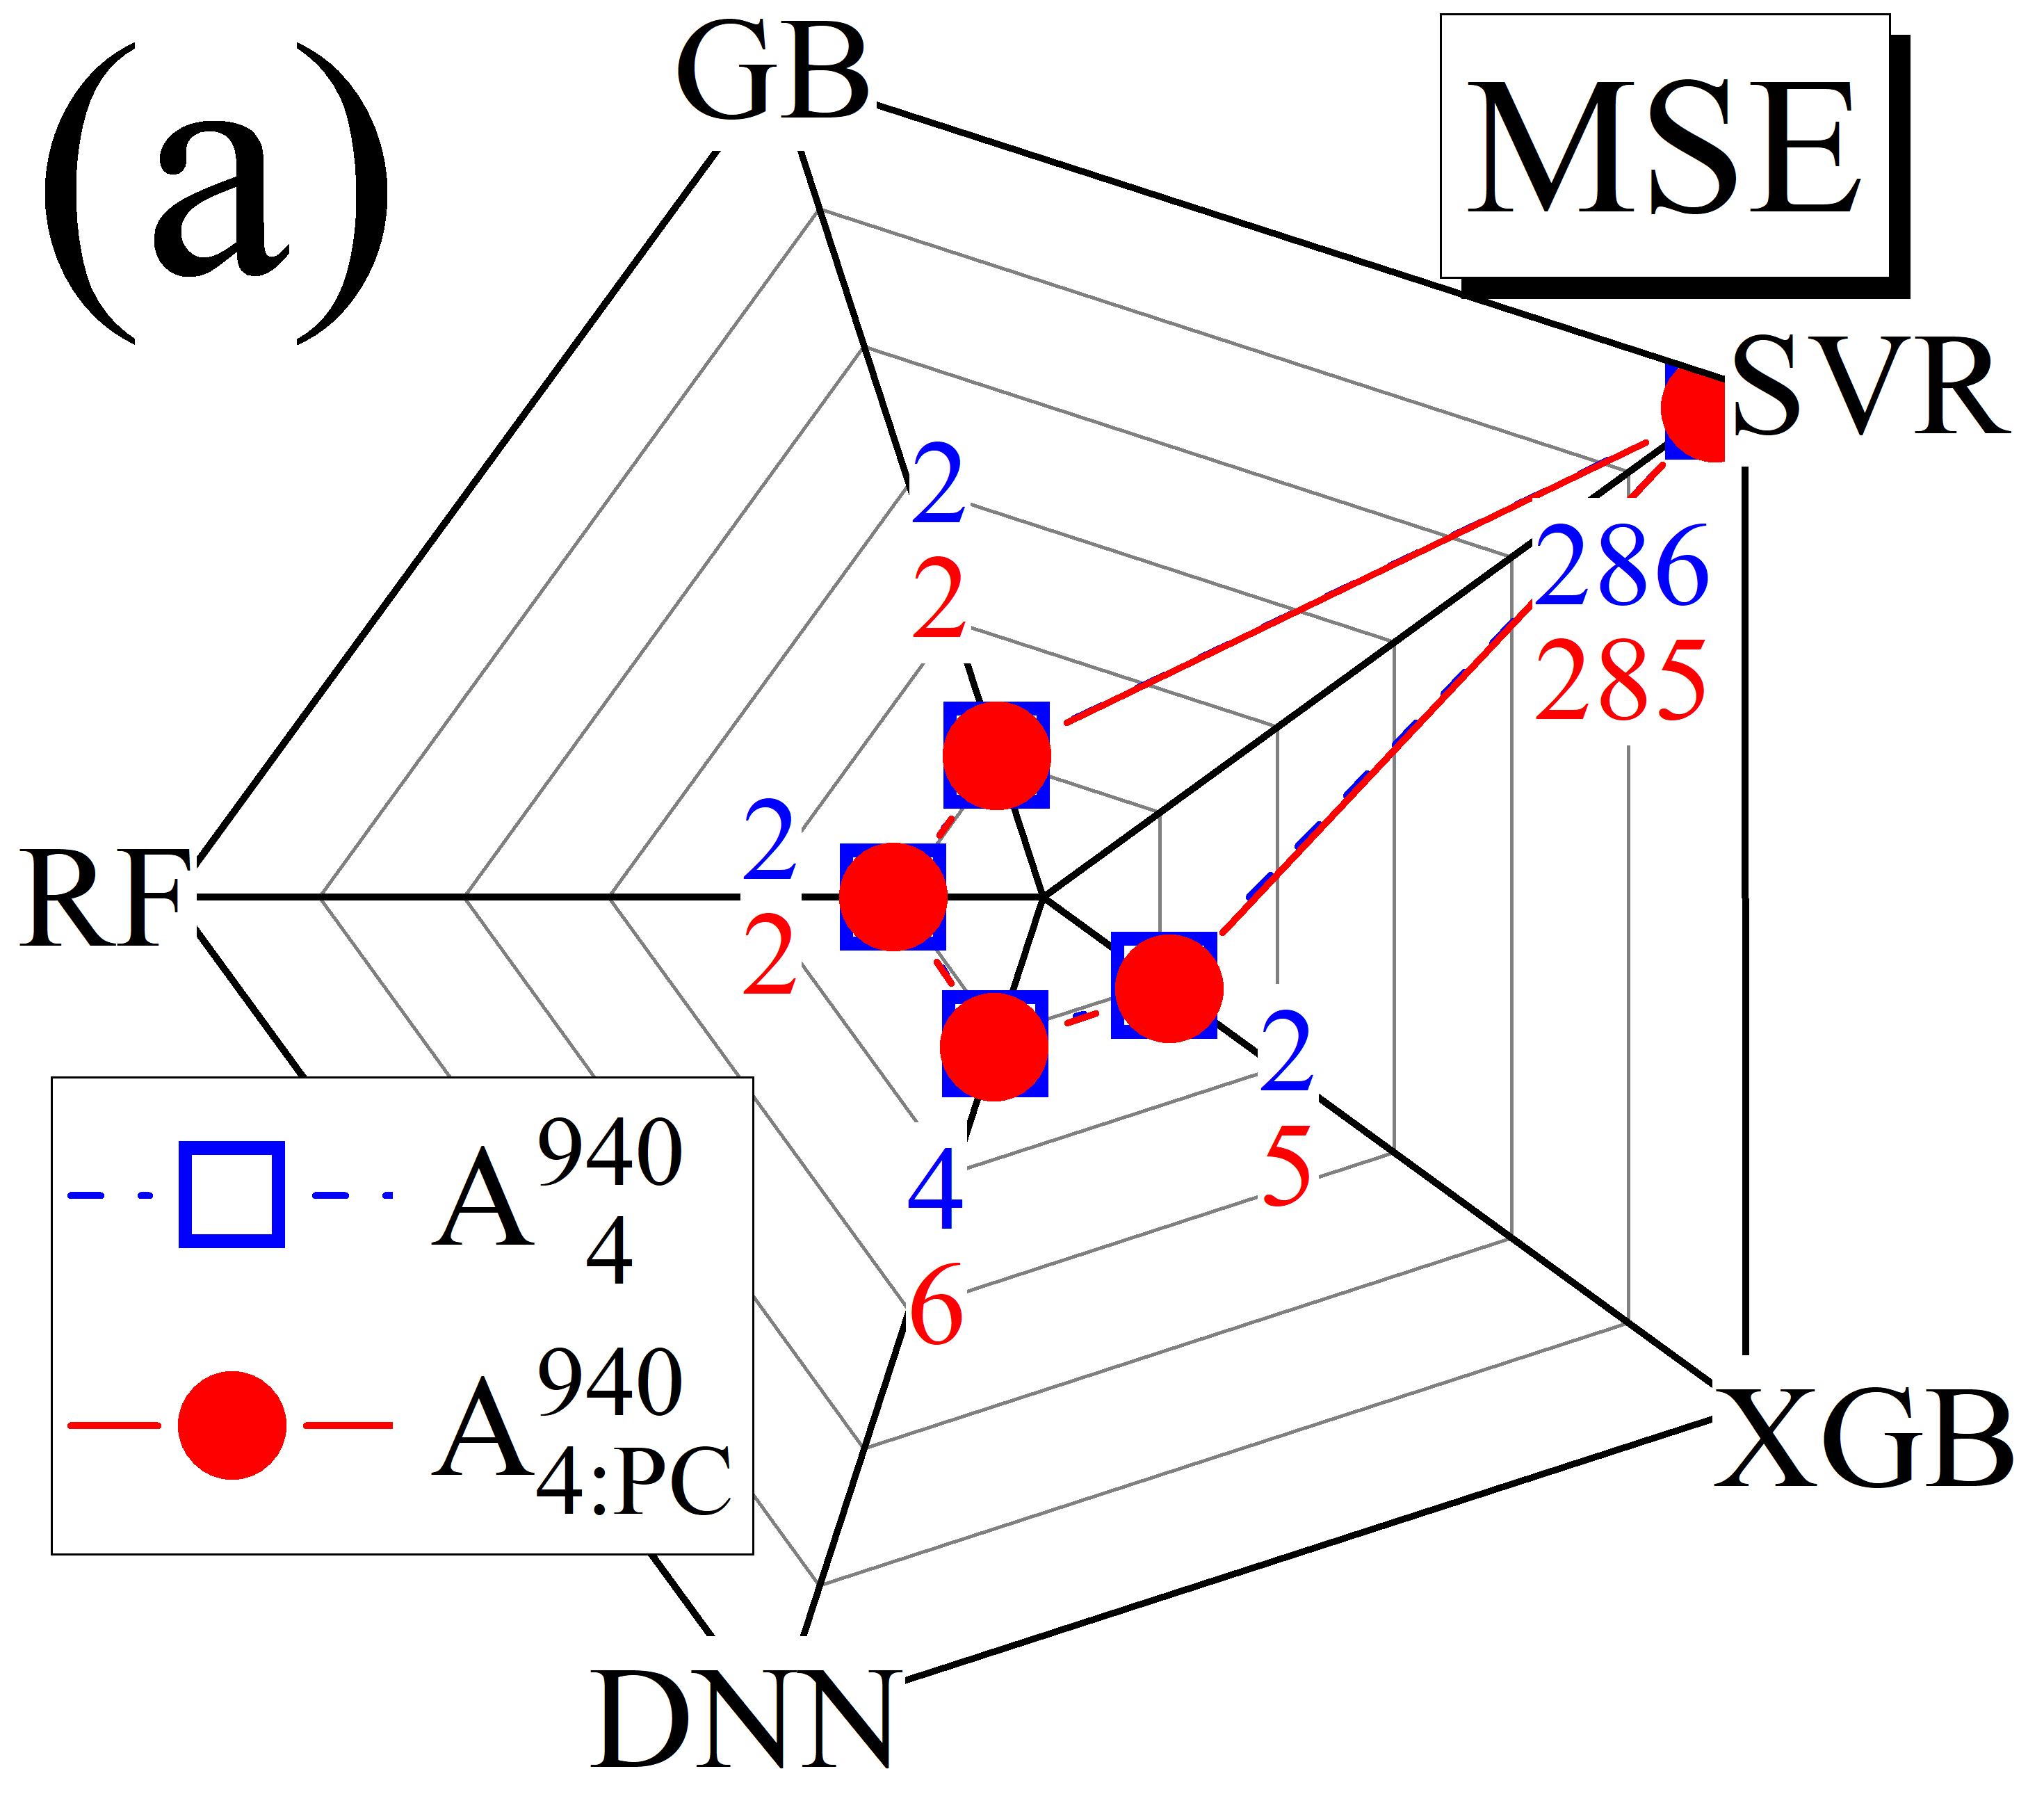
\includegraphics[width=0.4\linewidth]{Fig7a.png}
     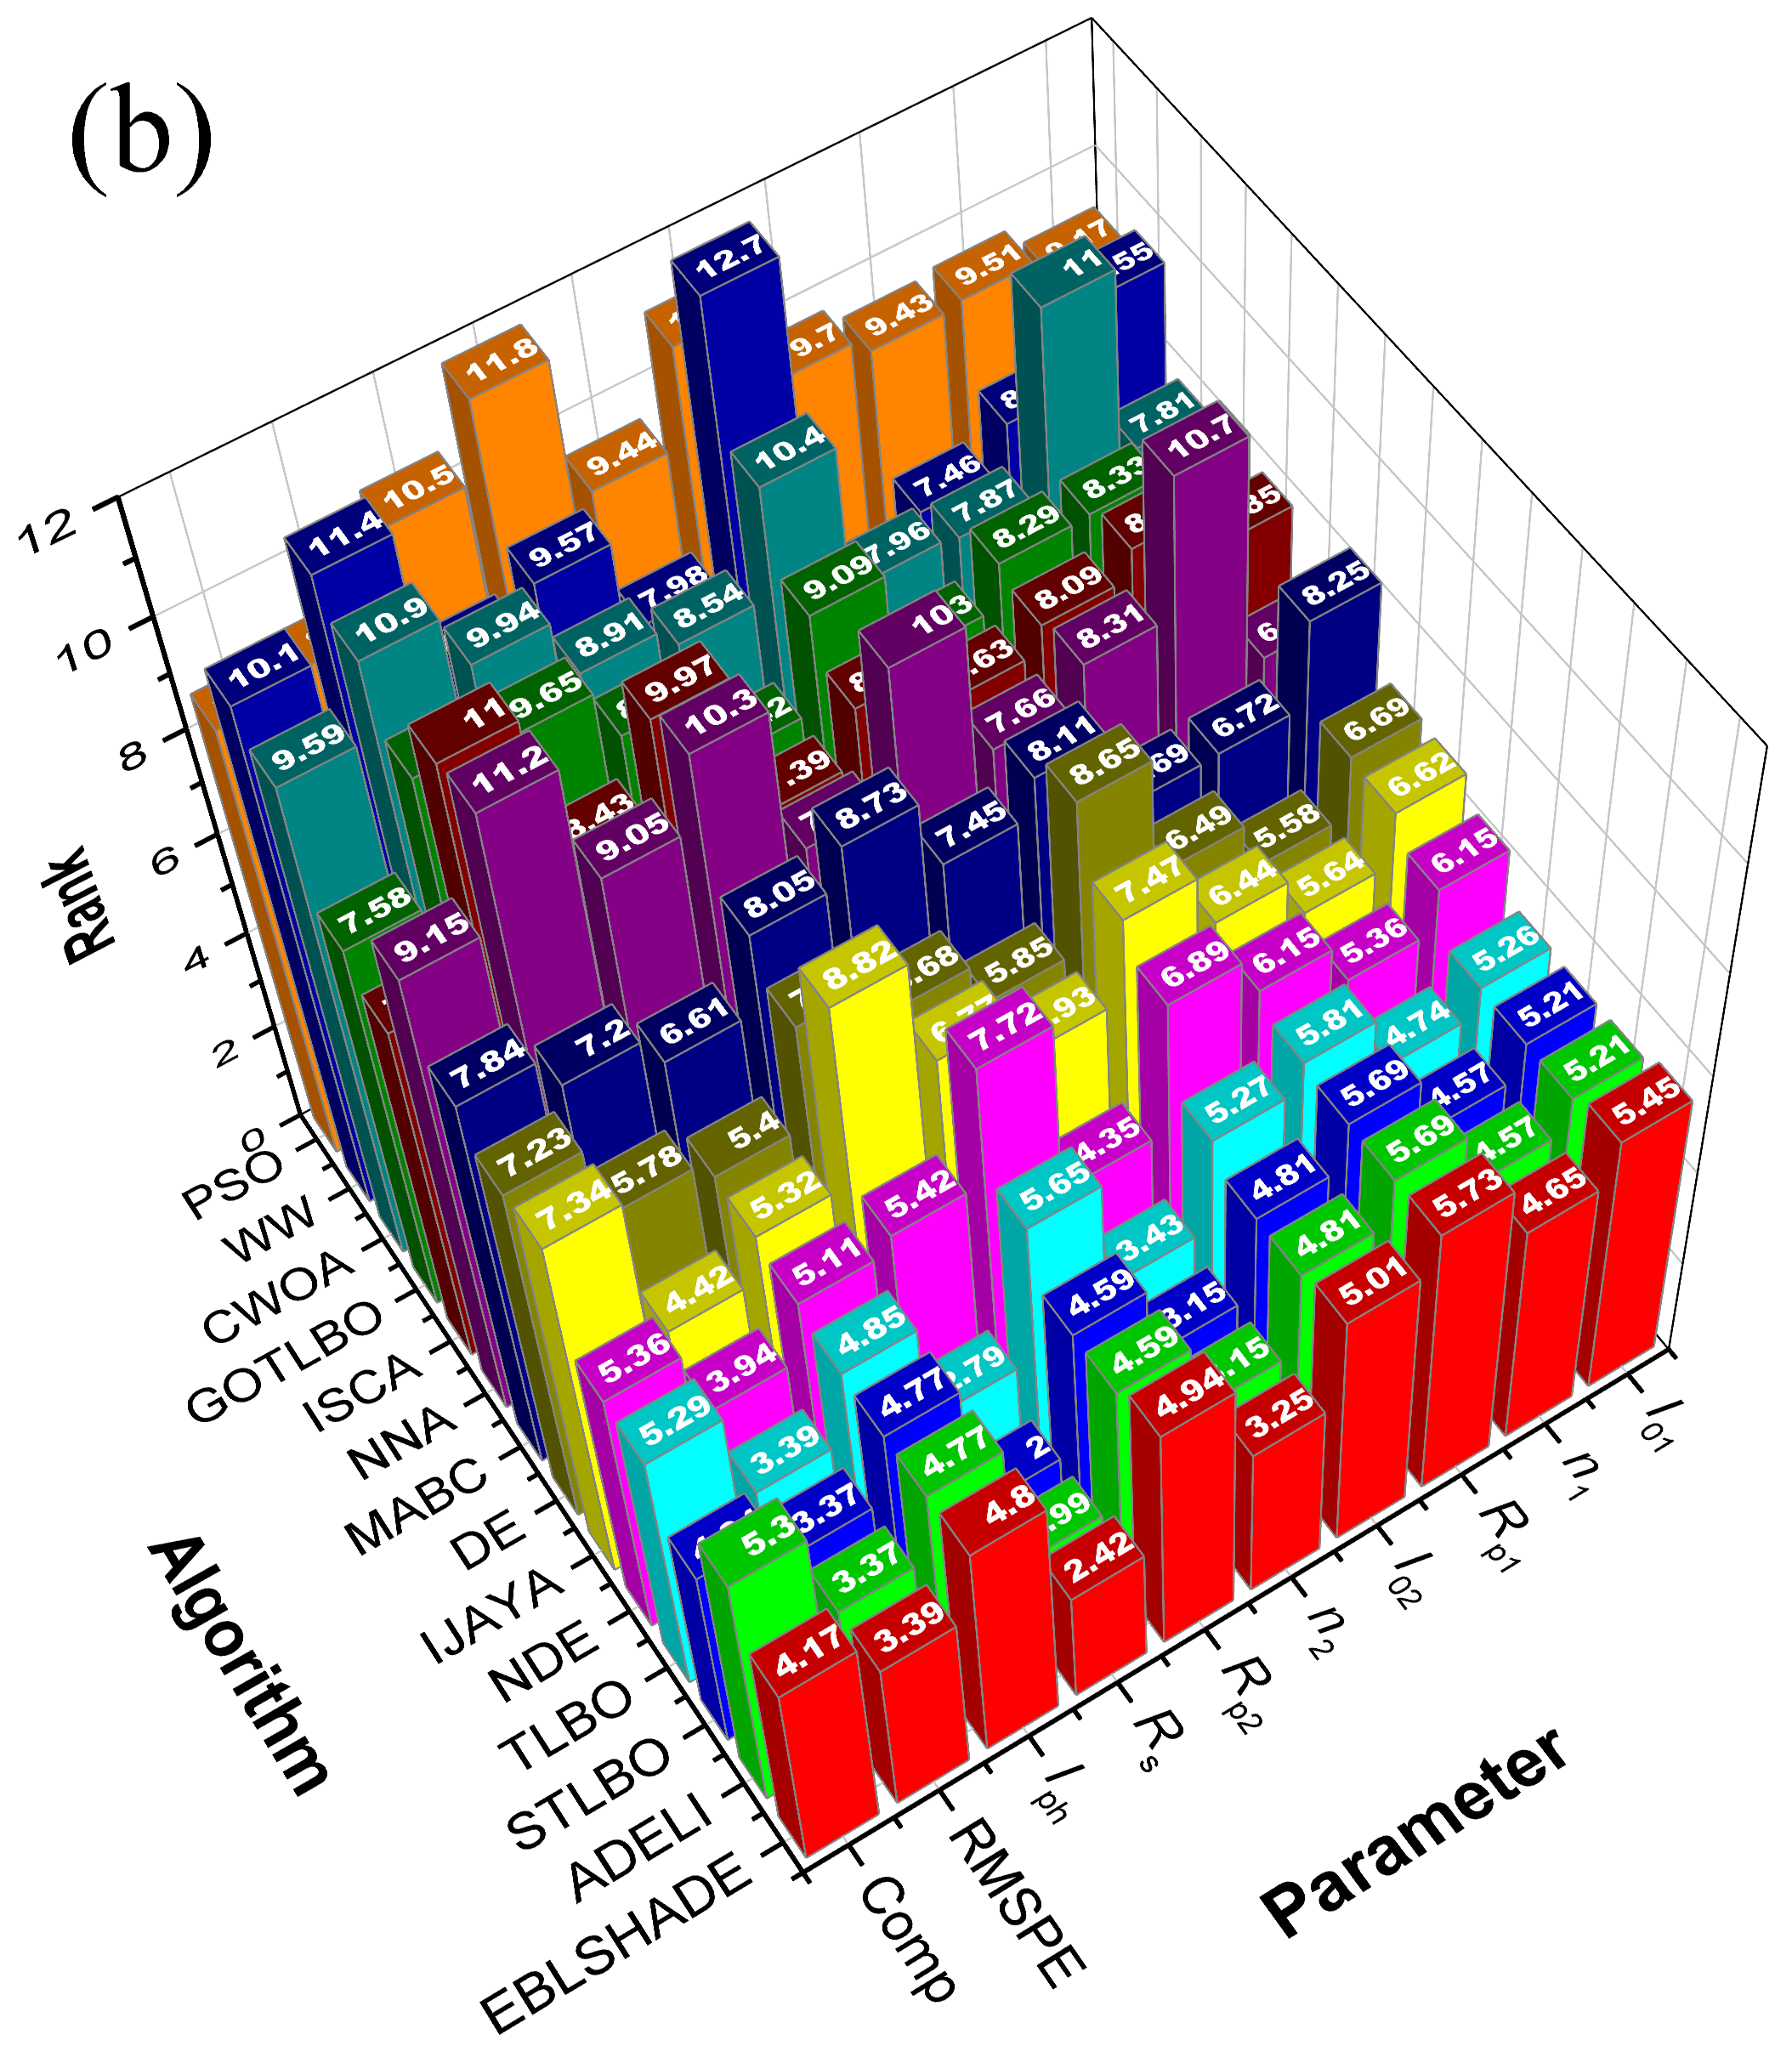
\includegraphics[width=0.4\linewidth]{Fig7b.png}
	  \caption{Relative changes in open-circuit voltage caused by a complete
       dissociation of Fe$_i$B$_s$ pairs as a function of iron concentration (a) and
       temperature (b) for SSC with $d_p=380$~$\mu$m and $N_\mathrm{B}=1.36\times10^{15}$~cm$^{-3}$
       in the case of monochromatic (940~nm) illumination.
       The marks are the experimental results, the lines are the simulation results.
       $W_\mathrm{ill}$, Wm$^{-2}$: 5 (marks and solid lines), 10 (dotted lines).
       Different lines and marks correspond to different temperatures (a) or $N_\mathrm{Fe}$ values (b) --- see legends.
}\label{fig7}
\end{figure}

\subsection{Fill factor}
The fill factor is another defining term in the overall behavior of a solar cell.
$FF$ is the ratio of the maximum obtainable power to the product of short circuit current and open-circuit voltage.
In general, $FF$ depends on both $I_\mathrm{SC}$ and $V_\mathrm{OC}$. 
However, it can be shown that it is mainly determined by the $V_\mathrm{OC}$ value. 
Indeed, it is shown \cite{YangHandbookPVSi} within the single-diode model
\begin{equation}
\label{eqFF1}
    FF \approx \frac{\upsilon_\mathrm{OC}-\ln\left(1+\upsilon_\mathrm{OC}\right)}{\upsilon_\mathrm{OC}+1} \,,
\end{equation}
with $\upsilon_\mathrm{OC}$ being the normalized open-circuit voltage 
$\upsilon_\mathrm{OC}=qV_\mathrm{OC}/nkT$.
Another well--known empirical relation for the maximum achievable fill factor of a solar cell is proposed by Green \cite{Green1981,Green1982}:
\begin{equation}
\label{eqFF2}
    FF \approx \frac{\upsilon_\mathrm{OC}-\ln\left(0.72+\upsilon_\mathrm{OC}\right)}{\upsilon_\mathrm{OC}+1} \,.
\end{equation}
Thus, all factors changing $V_\mathrm{OC}$ lead also to $FF$ change.
However, $V_\mathrm{OC}$ is present in both the numerator and denominator of Eqs.~(\ref{eqFF1})-(\ref{eqFF2}), 
and therefore, the expected changes in the fill factor compared to the open-circuit should be smaller.

Recently, Bothe et~al. \cite{Bothe2023} suggested explicit expressions for the FF regarding other characteristic solar cell parameters.
Specifically, for $p$--type SSCs and intrinsic limits, the parameterization can be written as follows:
\begin{equation}
\label{eqFF3}
    FF = \frac{90.4924}{d_p^{0.00220}}\left[0.9478+\frac{0.0519}{1+\left(\frac{\log N_\mathrm{B}}{17.3739 d_p^{-0.0093}}\right)^{76.3}}\right] \,,
\end{equation}
where
$d_p$ is expected to be in $\mu$m.
Additional recombination (e.g., Shockley–Read–Hall) leads to a decrease in $FF$ value \cite{Bothe2023}.

Figures S13-S16 in the Supplementary Material and Figure~\ref{fig8} illustrate the changes in fill factor due to iron defect variability. We can emphasize the following features of $\varepsilon FF$:
\begin{itemize}
    \item The changes in the fill factor are the smallest compared to the other parameters under consideration—maximum values of $\varepsilon FF$ do not exceed 10\%;
    \item At low boron concentrations ($N_\mathrm{B}<10^{16}$~cm$^{-3}$), the dependence of $\varepsilon FF$$\left(N_\mathrm{Fe}\right)$ is significantly non-linear: within the considered concentration range, we observe two regions of decrease and two regions of increase in the corresponding dependence;
    \item At low boron concentrations, the changes in the fill factor are positive, and unlike $\varepsilon V_\mathrm{OC}$ and $\varepsilon I_\mathrm{SC}$, AM1.5 illumination causes greater changes in $FF$ compared to monochromatic illumination; at high boron concentrations, $\varepsilon FF$ < 0 and does not exceed 4\%;
    \item With increasing temperature, there is an increase in the magnitude of $\varepsilon FF$, regardless of its sign;
    \item Increasing the base thickness causes a decrease in the $\varepsilon FF$ value (in general, a decrease in the fill factor is expected with increasing $d_p$ according to (\ref{eqFF3})); furthermore, this shift in the $\varepsilon FF$$\left(N_\mathrm{Fe}\right)$ dependence is towards lower iron concentrations. The effect of $d_p$ is more pronounced at low boron concentrations and under AM1.5 illumination;
    \item Under monochromatic illumination, the effect of intensity on the relative changes in the fill factor is quite significant ($\varepsilon FF$ can vary by a factor of 2 with a change in $W_\mathrm{ill}$ from 5 to 10~Wm$^{-2}$), and the impact depends on both the iron concentration (even with a change in sign) and on the temperature;
\end{itemize}

Figure~\ref{fig9} shows that the experimental dependencies $\varepsilon FF$$\left(N_\mathrm{Fe}\right)$ and $\varepsilon FF$$\left(T\right)$ are in good agreement with the calculated values. The quantitative agreement is, in our opinion, hampered  by the relatively low accuracy of $\varepsilon FF$ measurements, as well as the fact that the fill factor depends on series and shunt resistances \cite{Green1981,Green1982}; which were not taken into account in the simulation.

The observed features of $\varepsilon FF$ indicate that the fill factor is much less suitable for estimating iron concentration in CSEs compared to short-circuit current and even open-circuit voltage. $\varepsilon FF$ can only be used as an auxiliary parameter to refine $N_\mathrm{Fe}$, but in the case of monochromatic illumination, its intensity must be controlled with high accuracy.

\begin{figure}
	\centering
     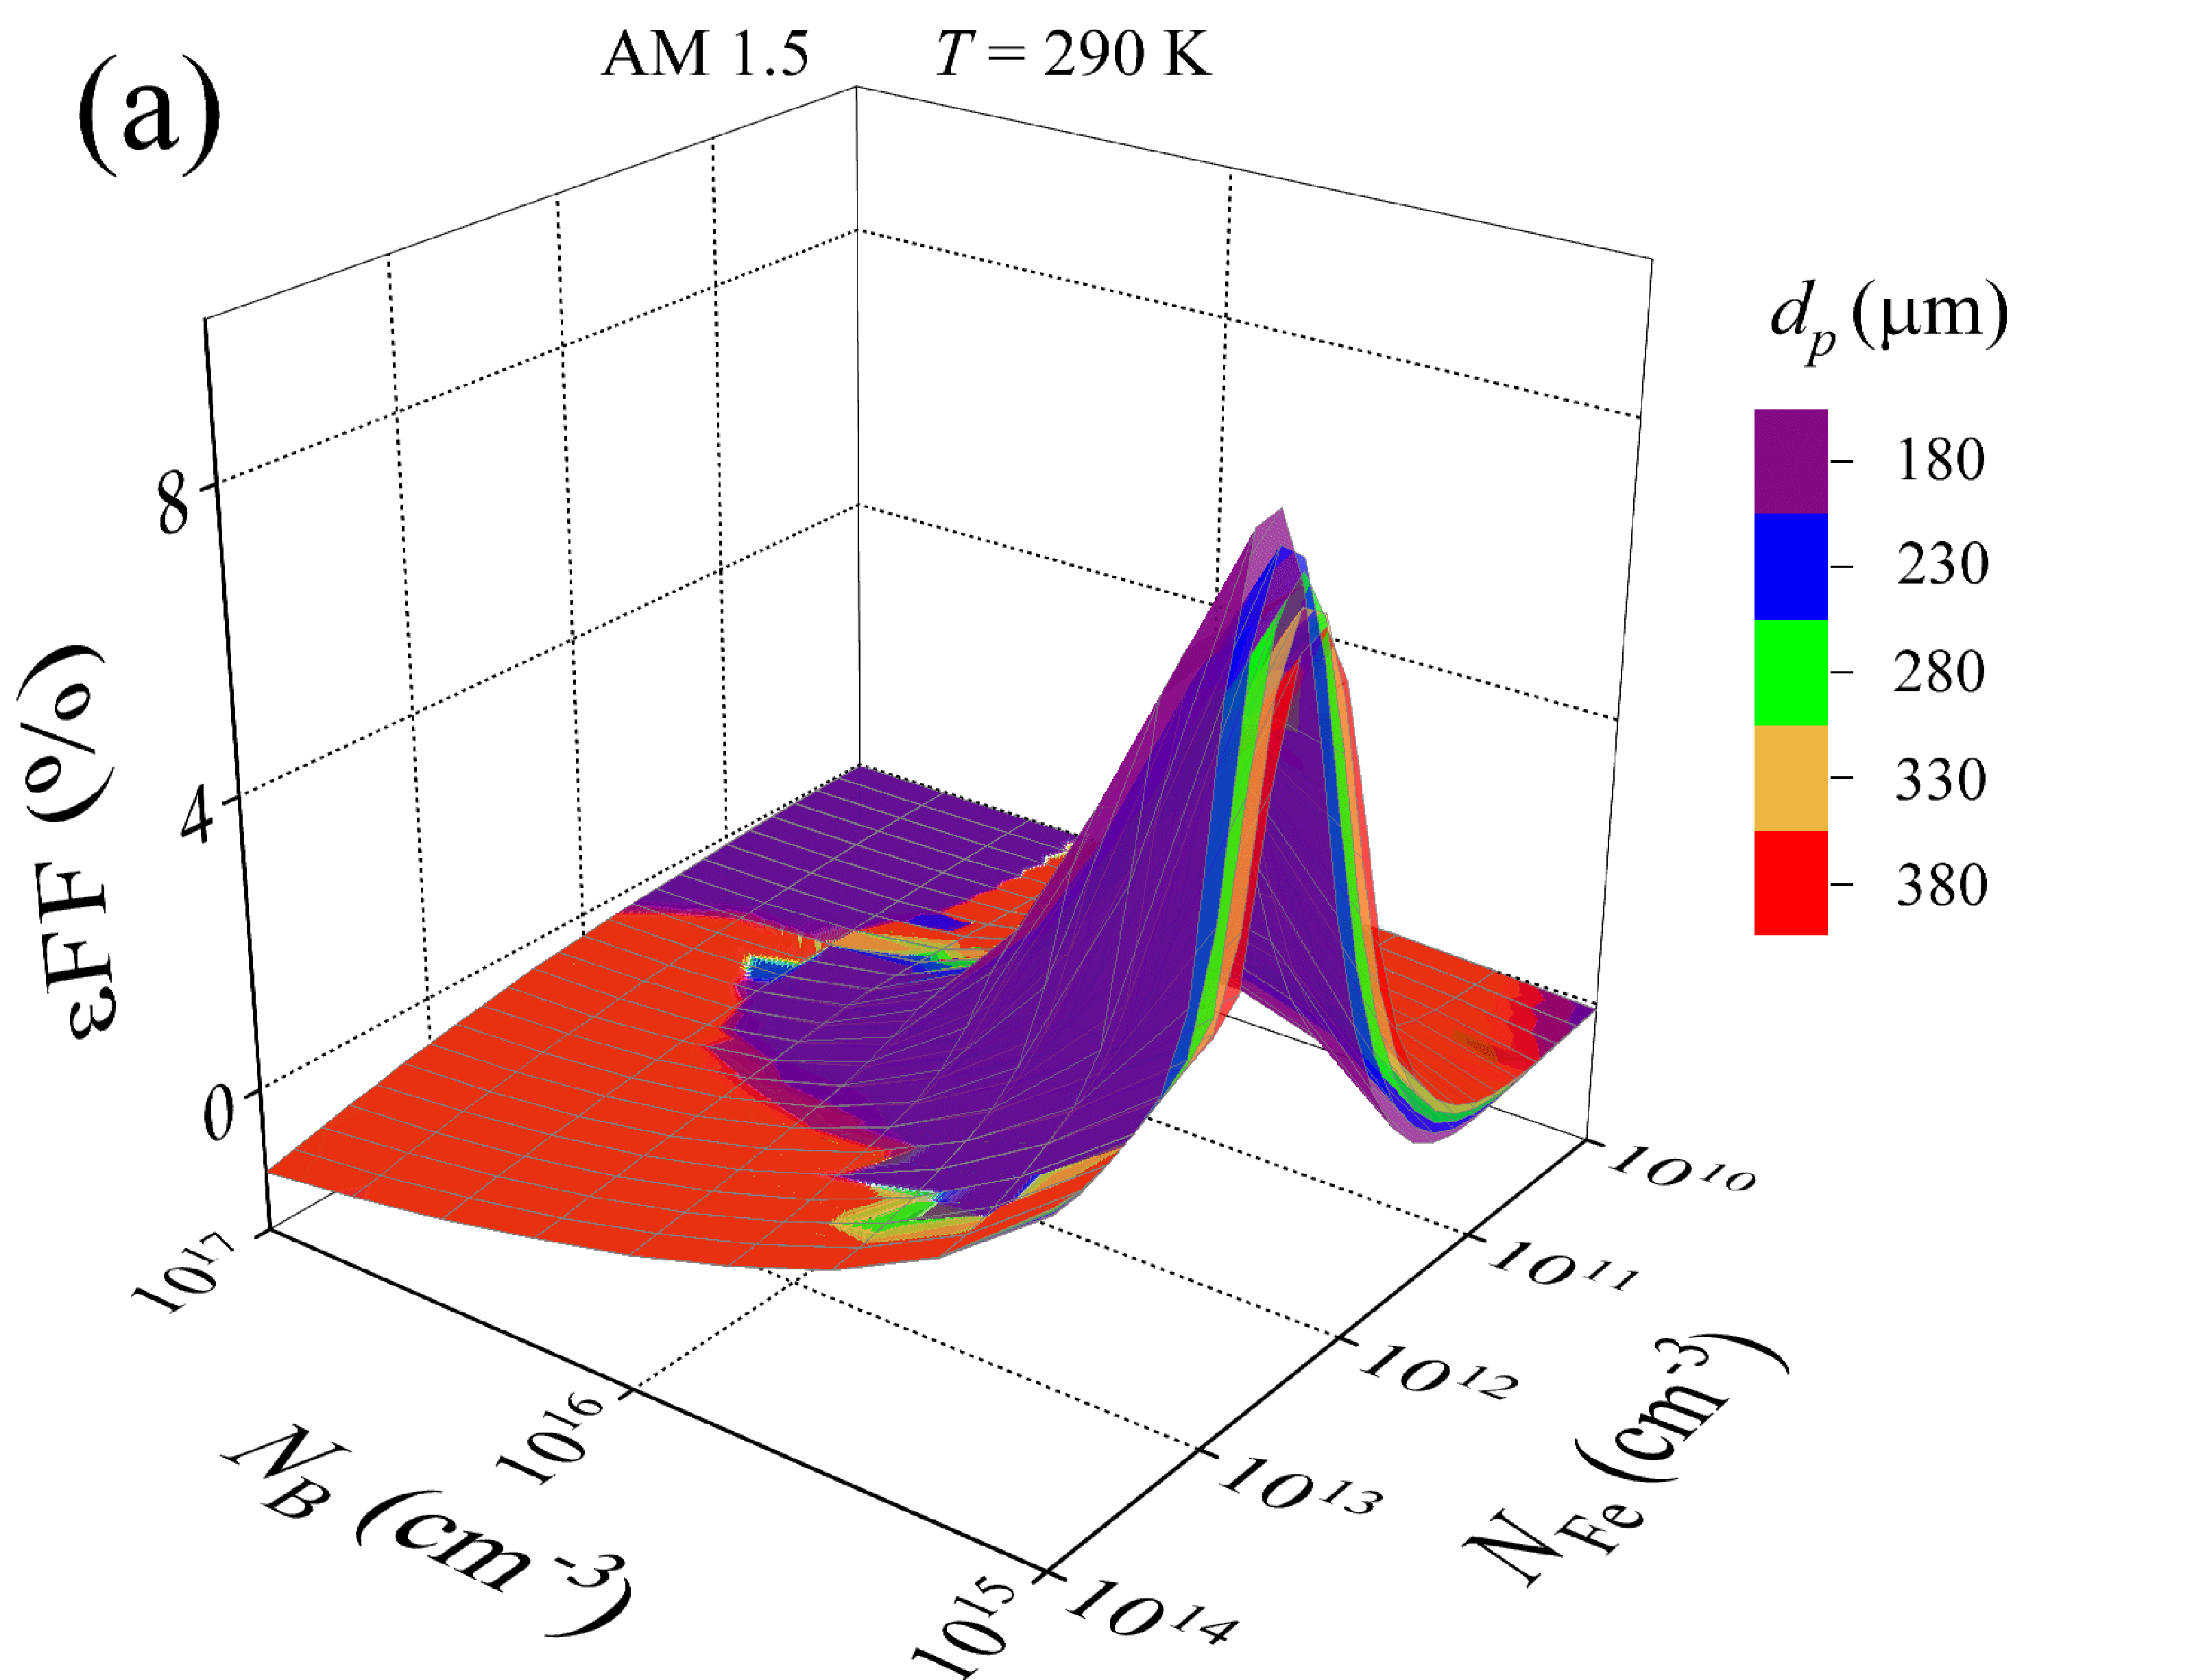
\includegraphics[width=0.49\linewidth]{Fig8a.png}
     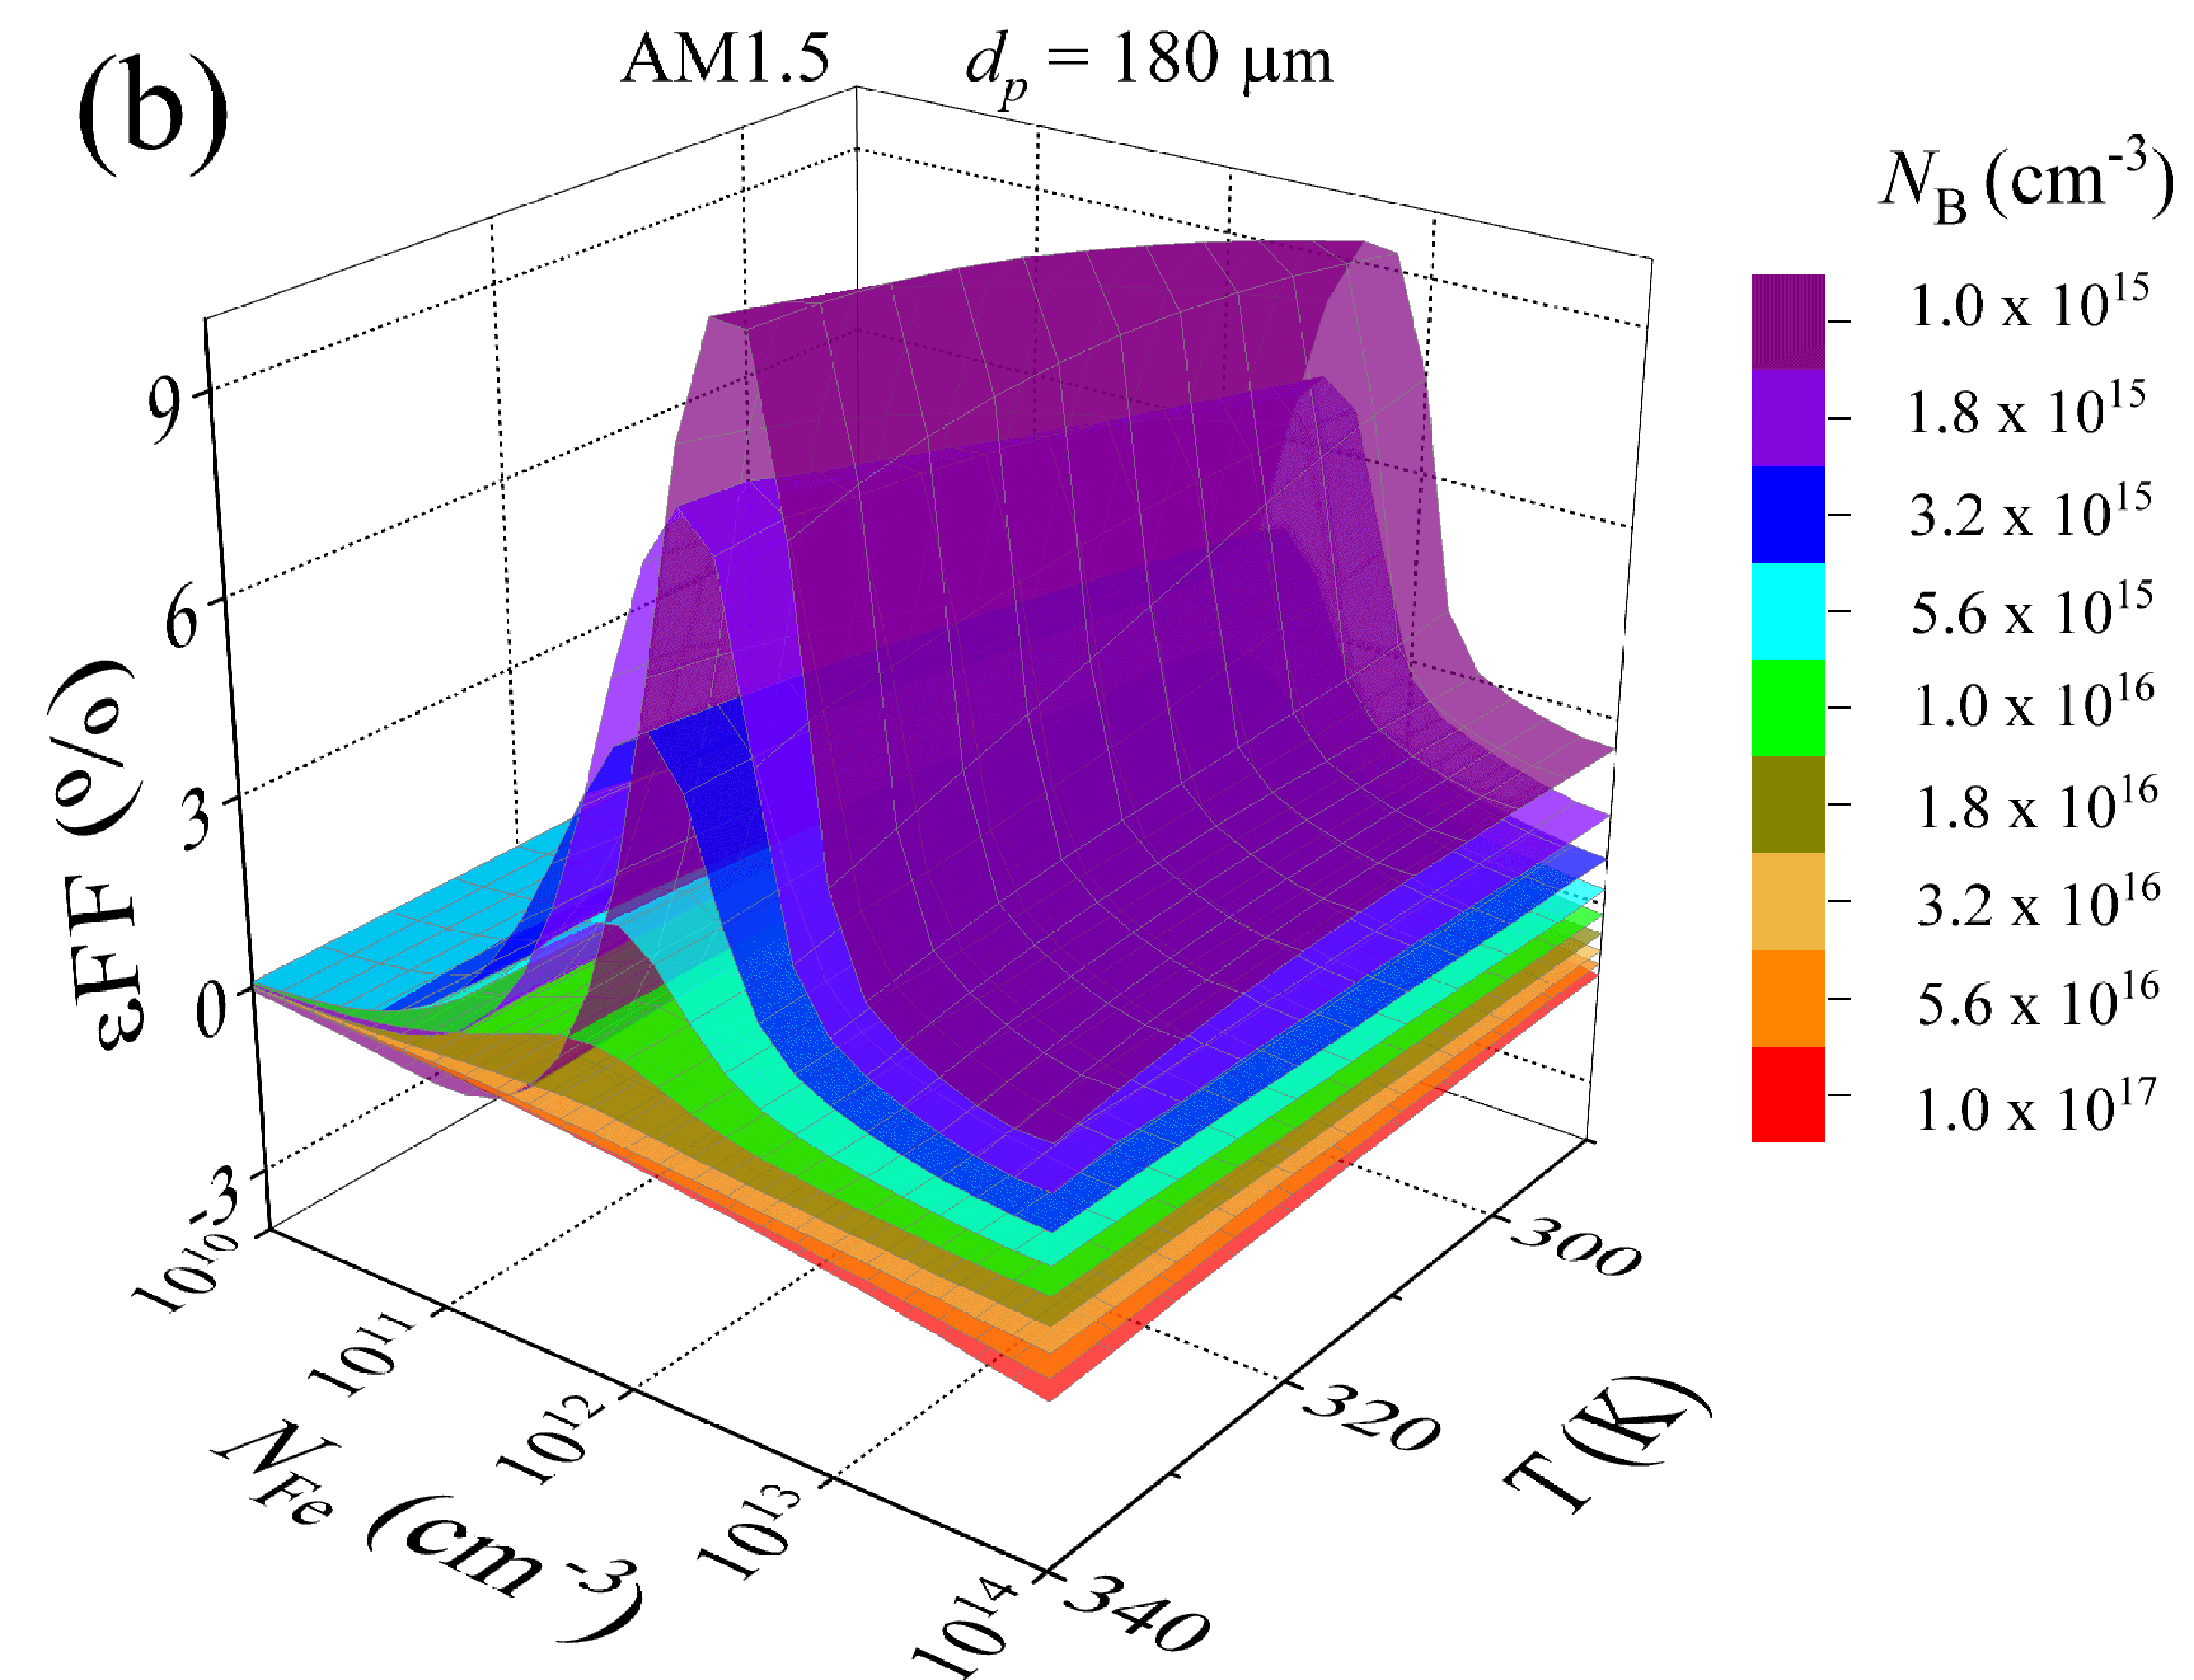
\includegraphics[width=0.49\linewidth]{Fig8b.png}
     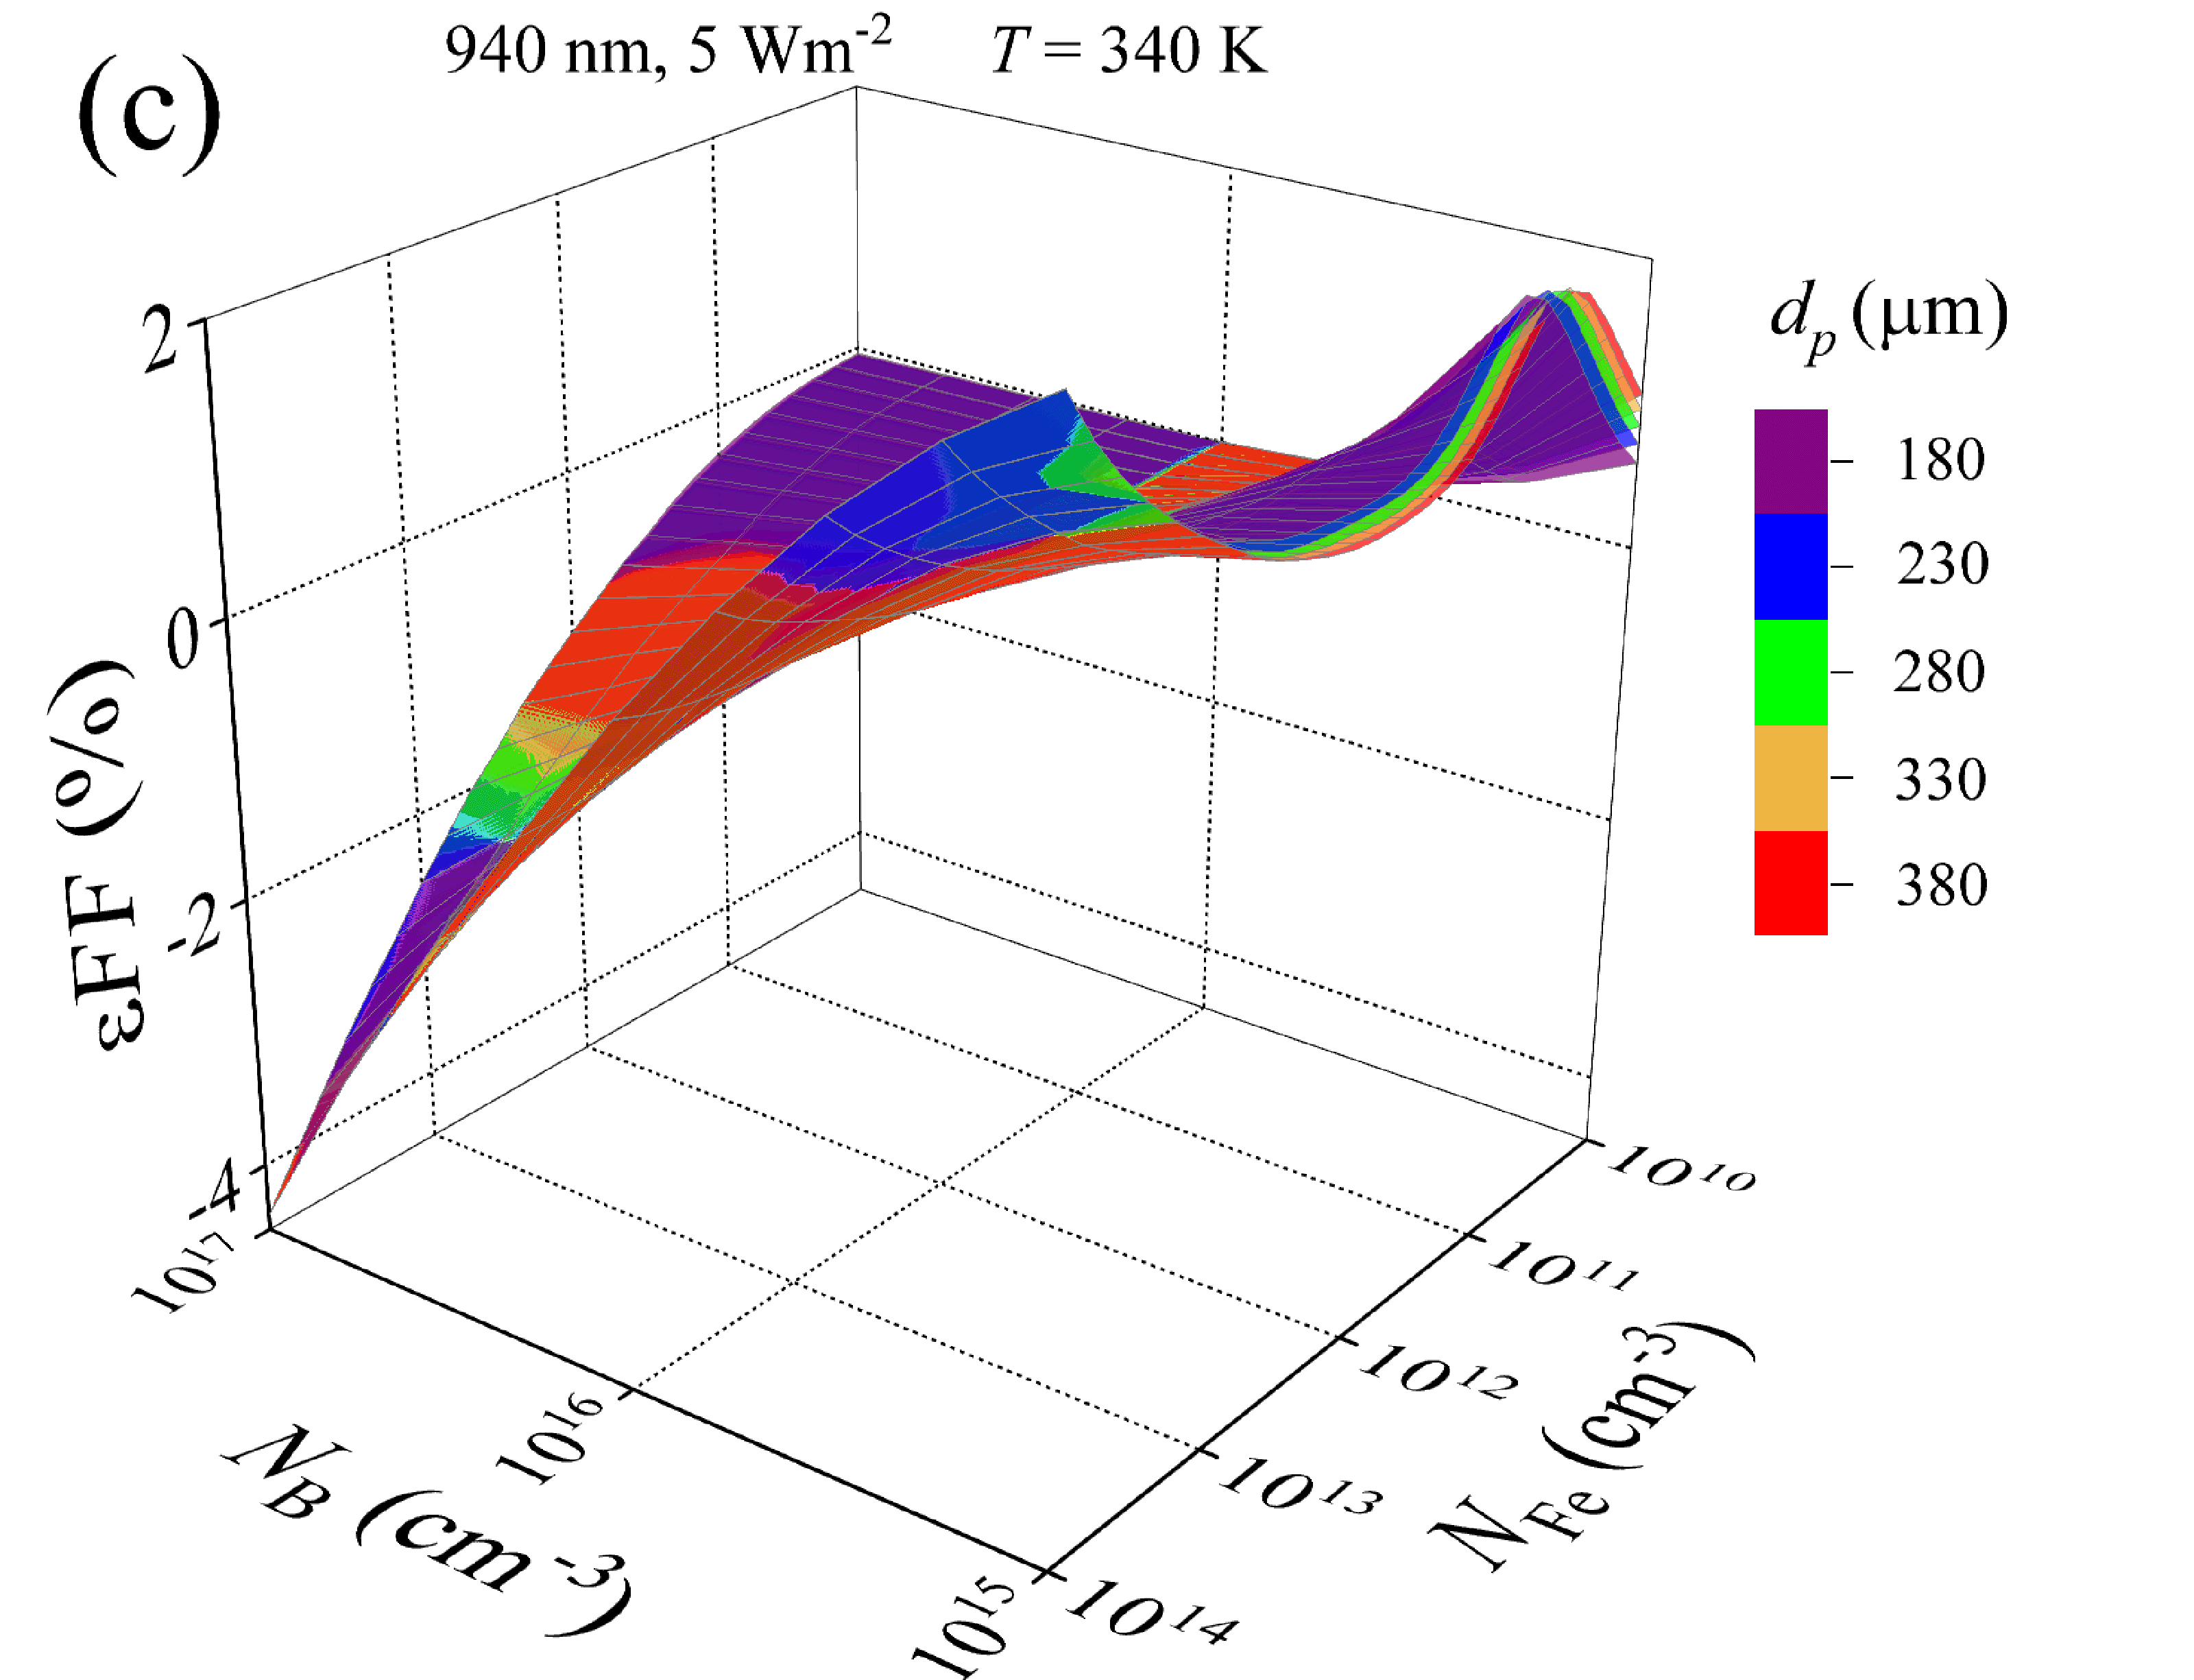
\includegraphics[width=0.49\linewidth]{Fig8c.png}
     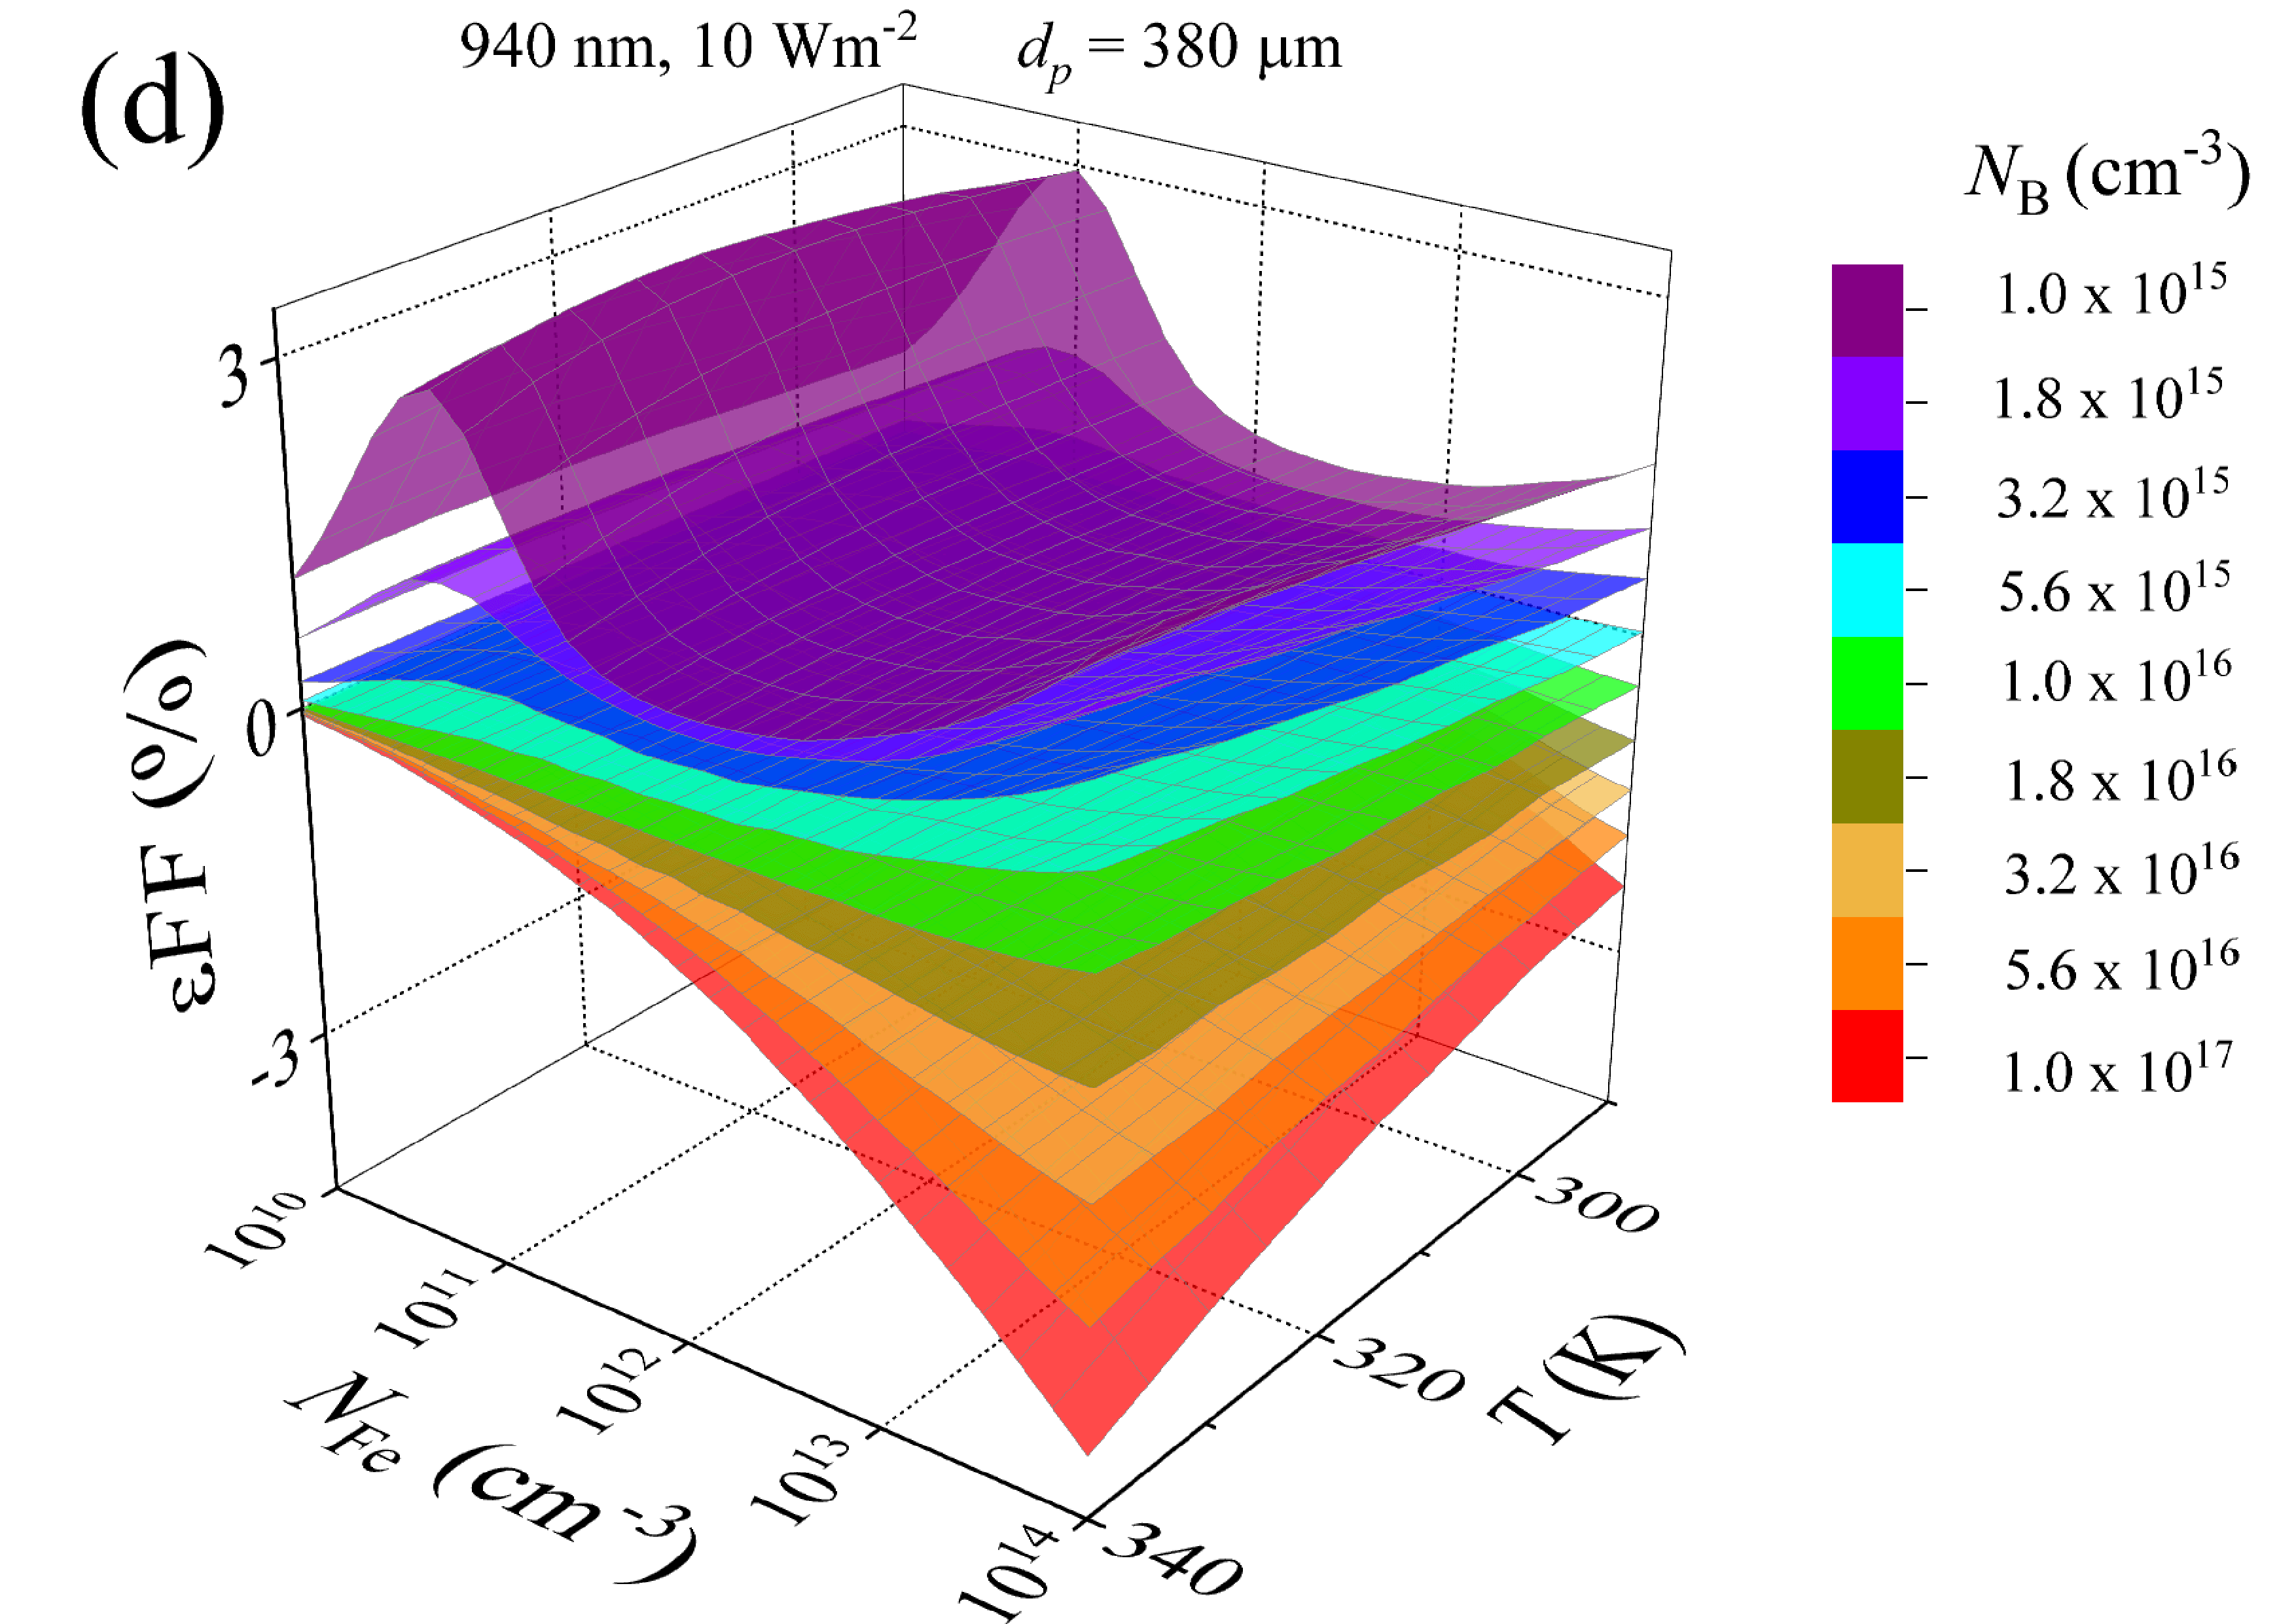
\includegraphics[width=0.49\linewidth]{Fig8d.png}
	  \caption{Relative changes in fill factor caused by a complete
       dissociation of Fe$_i$B$_s$ pairs as a function of
       iron concentration and
       doping level (panels a and c) or temperature (b, d).
       Illumination: AM1.5 (a, b), 940~nm 5~Wm$^{-2}$ (c),  940~nm 10~Wm$^{-2}$ (d).
       $T$, K: 290 (a), 340 (c).
       $d_p$, $\mu$m: 180 (b), 380 (d).
       Different surfaces correspond to different base depths (a, c) and doping levels (b, d).
}\label{fig8}
\end{figure}


\begin{figure}
	\centering
     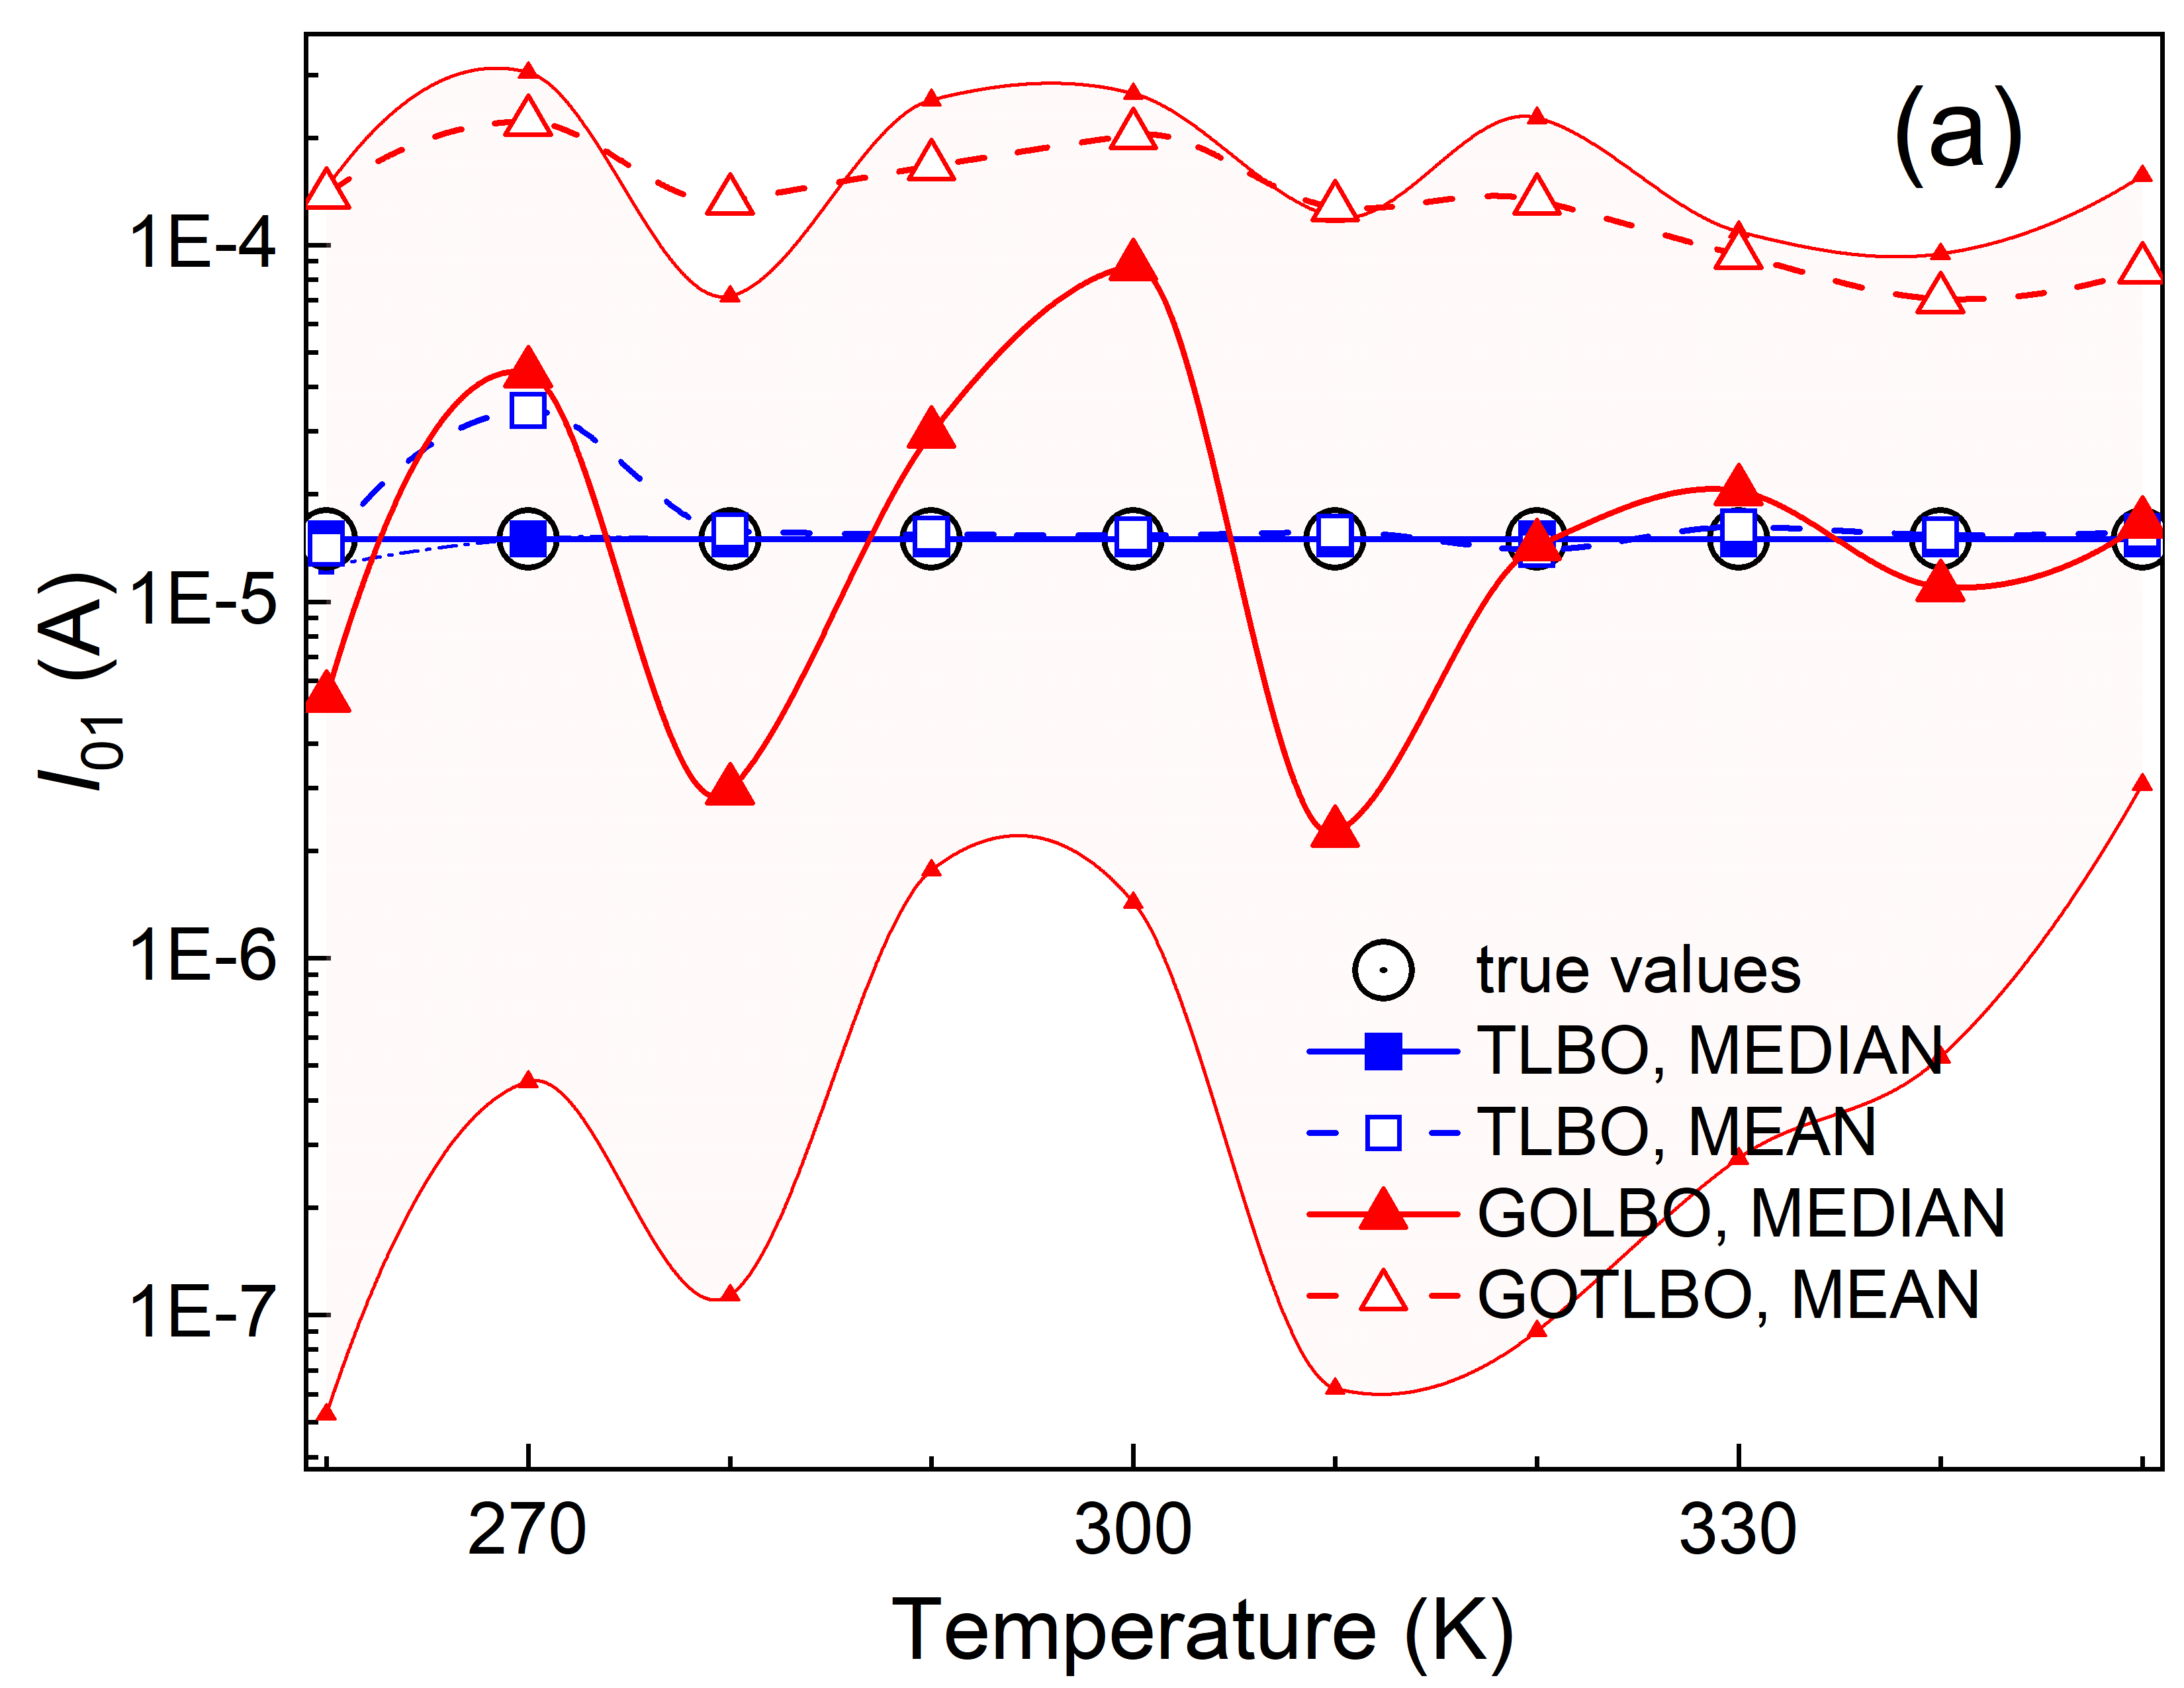
\includegraphics[width=0.4\linewidth]{Fig9a.png}
     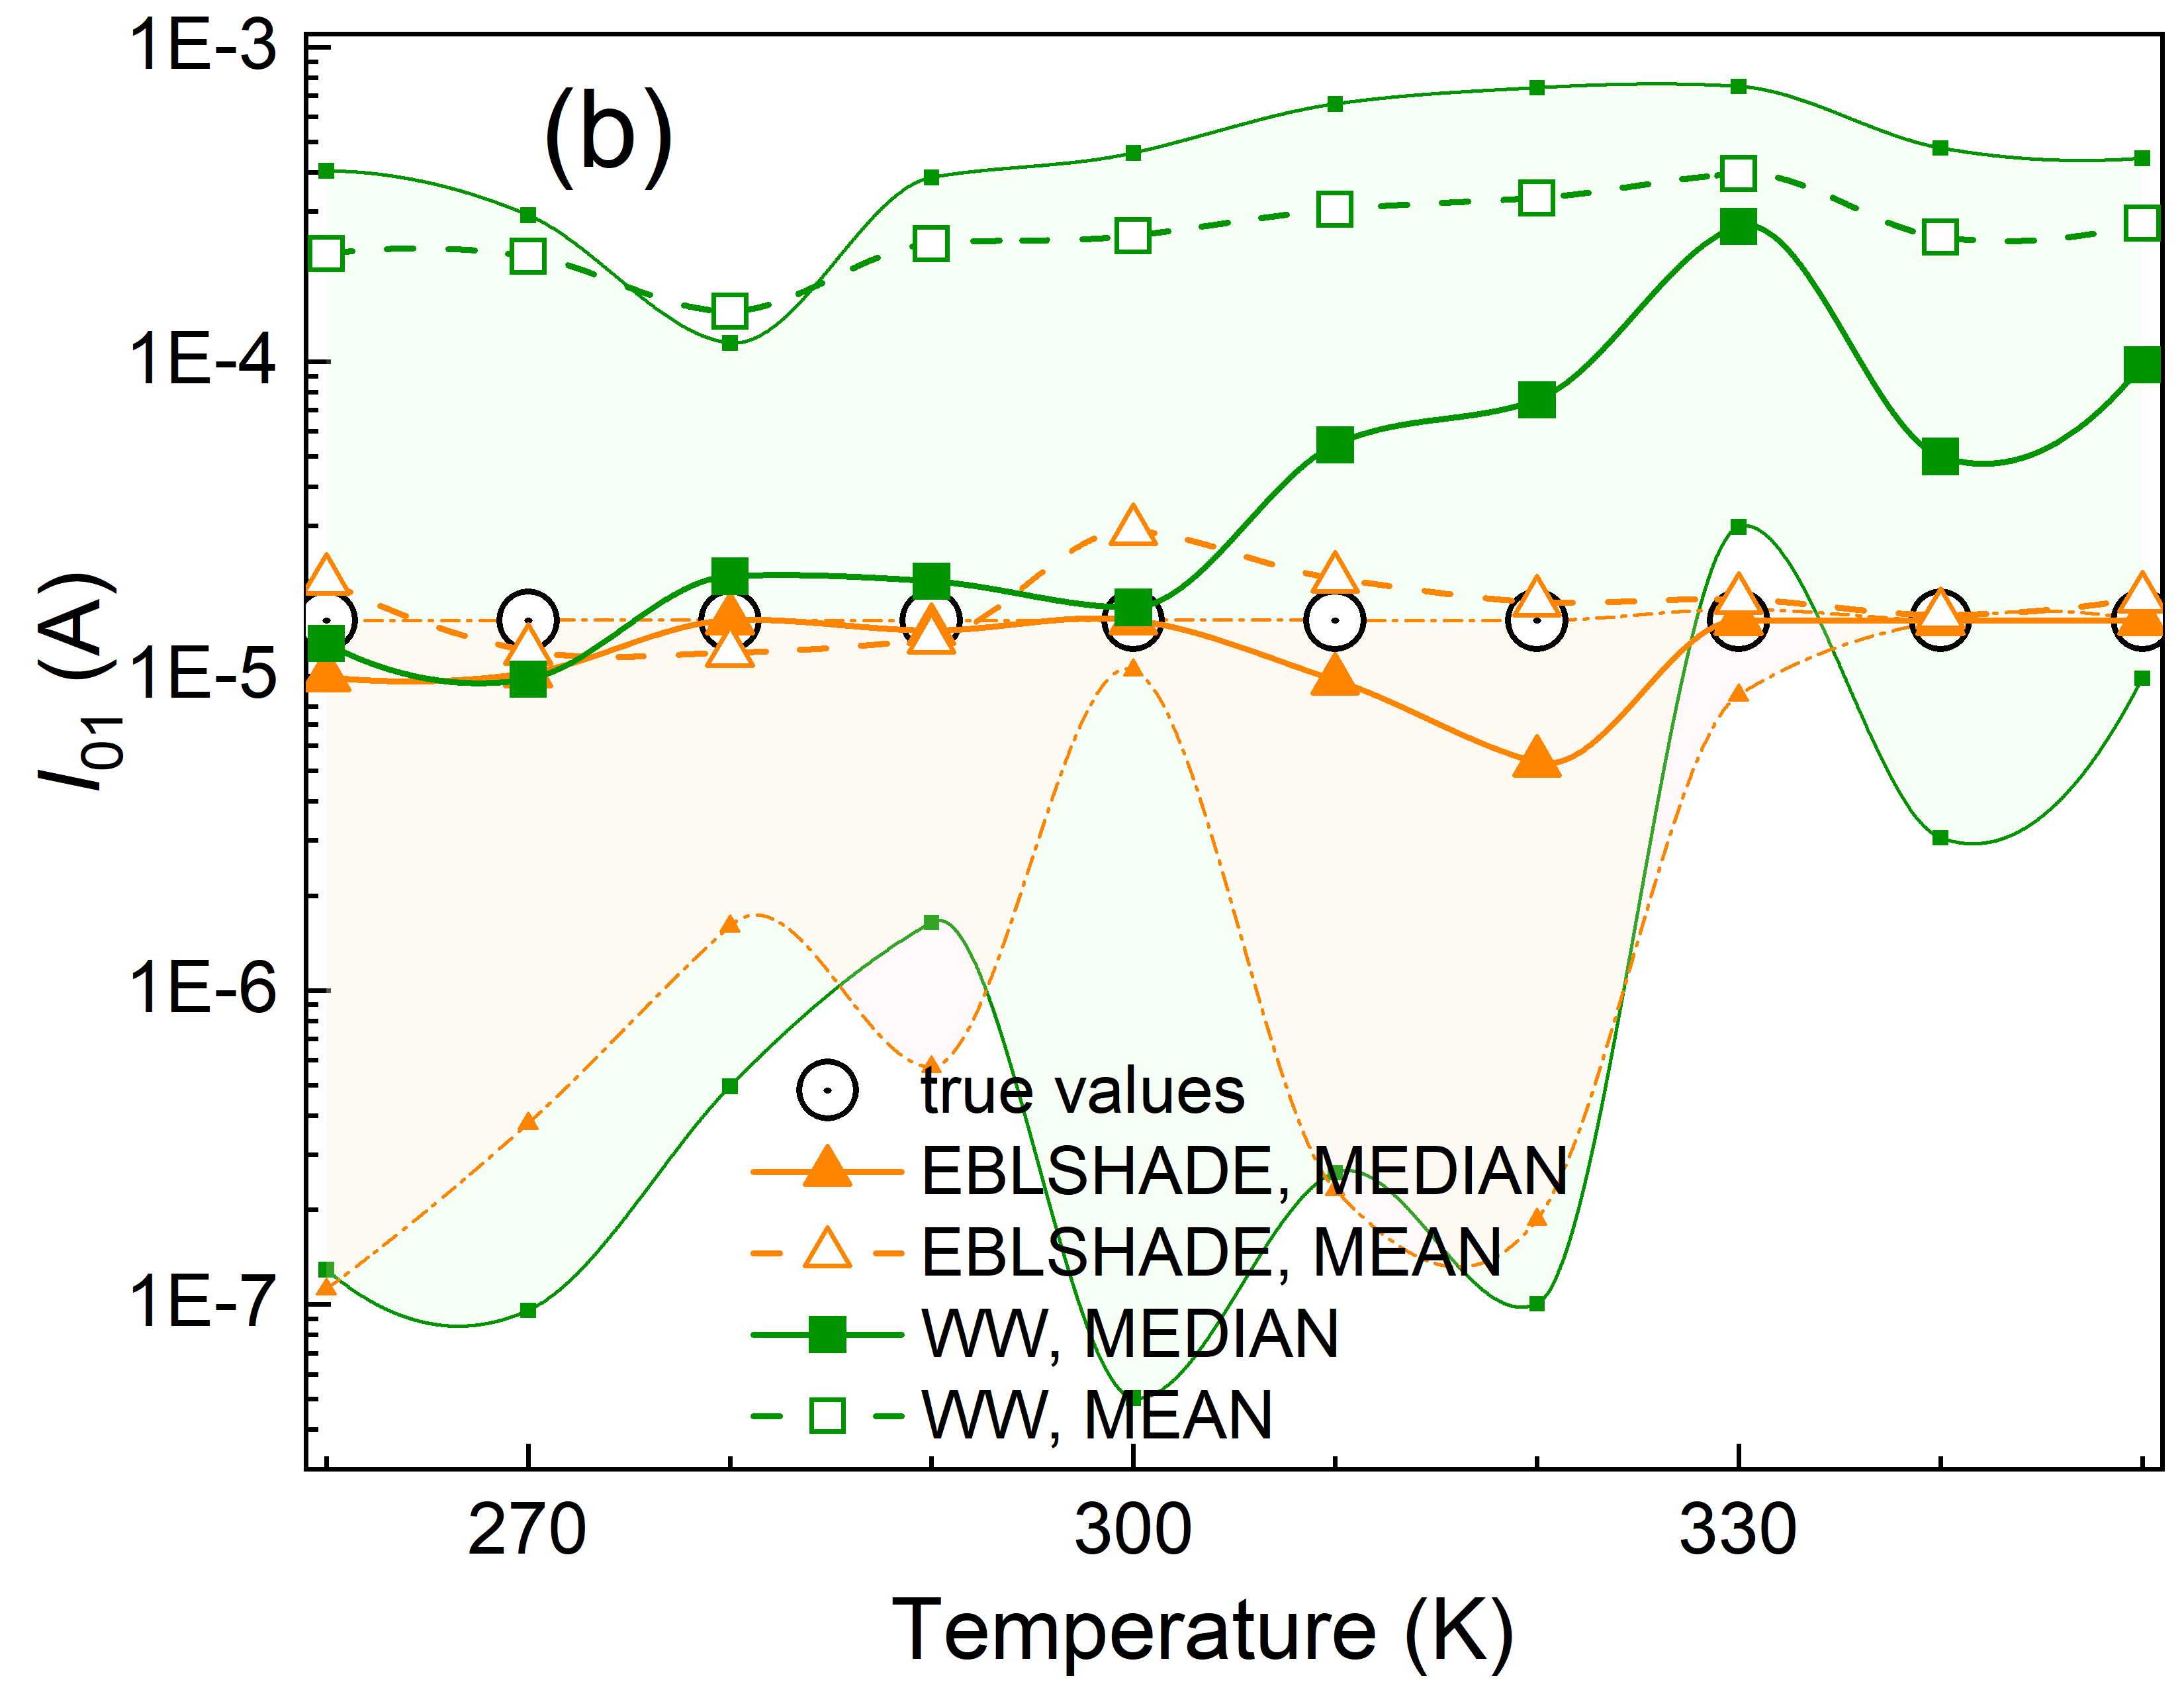
\includegraphics[width=0.4\linewidth]{Fig9b.png}
	  \caption{Relative changes in fill factor caused by a complete
       dissociation of Fe$_i$B$_s$ pairs as a function of iron concentration (a) and
       temperature (b) for SSC with $d_p=380$~$\mu$m and $N_\mathrm{B}=1.36\times10^{15}$~cm$^{-3}$
       in the case of monochromatic (940~nm) illumination.
       The marks are the experimental results, the lines are the simulation results.
       $W_\mathrm{ill}$, Wm$^{-2}$: 5 (marks and solid lines), 10 (dotted lines).
       Different lines and marks correspond to different temperatures (a) or $N_\mathrm{Fe}$ values (b) --- see legends.
}\label{fig9}
\end{figure}

\subsection{Solar Cell Efficiency}

The efficiency of a solar cell depends on all the photovoltaic conversion parameters discussed earlier: 
\begin{equation}
\label{eq11}
    \eta = \frac{I_\mathrm{SC}V_\mathrm{OC}FF}{W_\mathrm{ill}A},
\end{equation}
where $A$ is the illuminated area of the solar cell. Considering the differential of formula (\ref{eq11}):
\begin{equation}
\label{eq12}
    d\eta = \frac{dI_\mathrm{SC}}{I_\mathrm{SC}}+\frac{dV_\mathrm{OC}}{V_\mathrm{OC}}+\frac{dFF}{FF},
\end{equation}
a cumulative effect on the relative changes in efficiency can be expected. Figure~\ref{fig10} shows the calculation results related to the efficiency of the solar cell; figures S17-S20 provide more detailed information on these.

As evident from the data provided, the main features of the $\varepsilon \eta$ dependencies on solar cell parameters and temperature are consistent with those observed for $\varepsilon I_\mathrm{SC}$. However, we can observe a few differences: 1) the amplitudes of the changes in $\varepsilon \eta$ are larger (reaching up to 50\% for AM1.5 and 200\% for 940~nm), which is reasonably expected based on formula (\ref{eq12}) and more convenient for estimating iron concentration; 2) For AM1.5, in the region of $N_\mathrm{B}<5\times10^{15}$~cm$^{-3}$, a non-monotonic dependence of $\varepsilon \eta$$\left(N_\mathrm{Fe}\right)$ is observed, which makes it impossible to use relative changes in efficiency as a single parameter for estimating iron concentration under these conditions; 3) The existing dependence of $\varepsilon \eta$ on the intensity of the monochromatic illumination is weak and does not hinder the use of $\varepsilon \eta$ to determine $N_\mathrm{Fe}$, even with not very precise measurements of $W_\mathrm{ill}$; 4) The temperature dependence of $\varepsilon \eta$ is weaker compared to $\varepsilon I_\mathrm{SC}$.

Figure~\ref{fig11} shows the experimental and calculated values of changes in the efficiency of the solar cell with a 380~$\mu$m base thickness and a doping concentration of $1.36\times10^{15}$~cm$^{-3}$. We applied the same correction factor $C_\mathrm{cor}$ = 1.4 to both the experimental data and the short-circuit current. The data align pretty well, which indicates that inaccuracies typical of $V_\mathrm{OC}$ and $FF$ do not dominate.

\begin{figure}
	\centering
     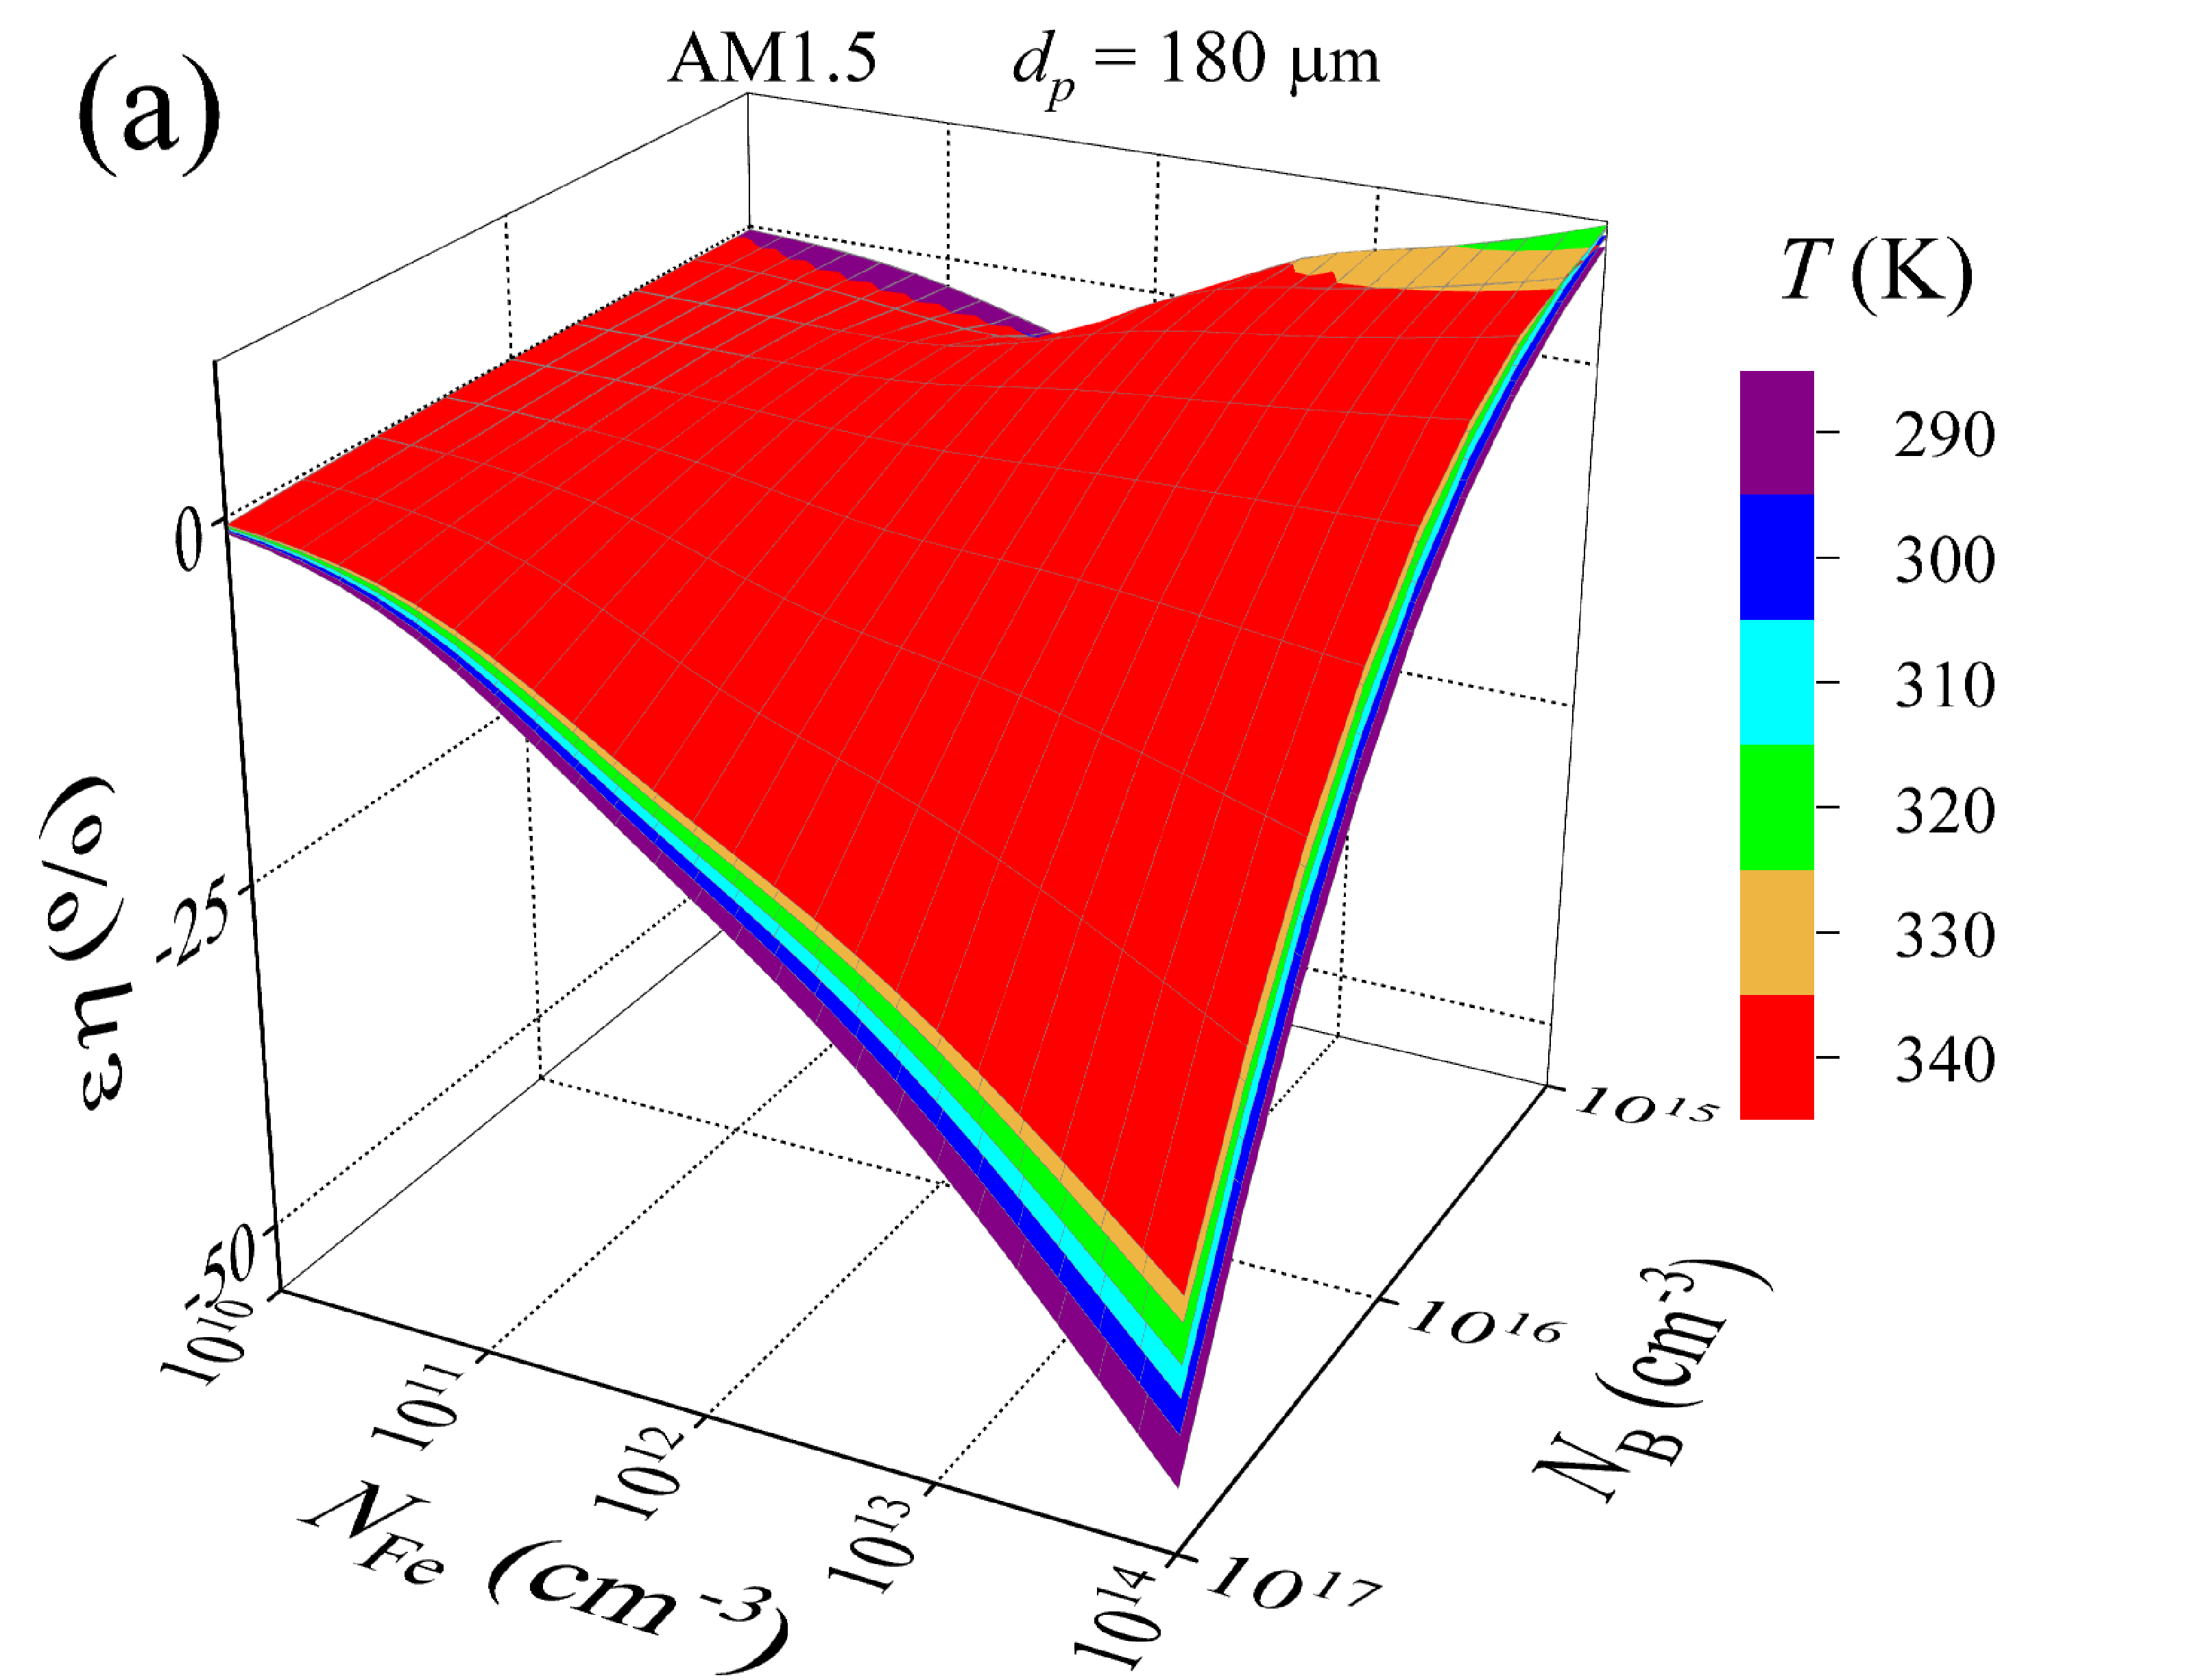
\includegraphics[width=0.49\linewidth]{Fig10a.png}
     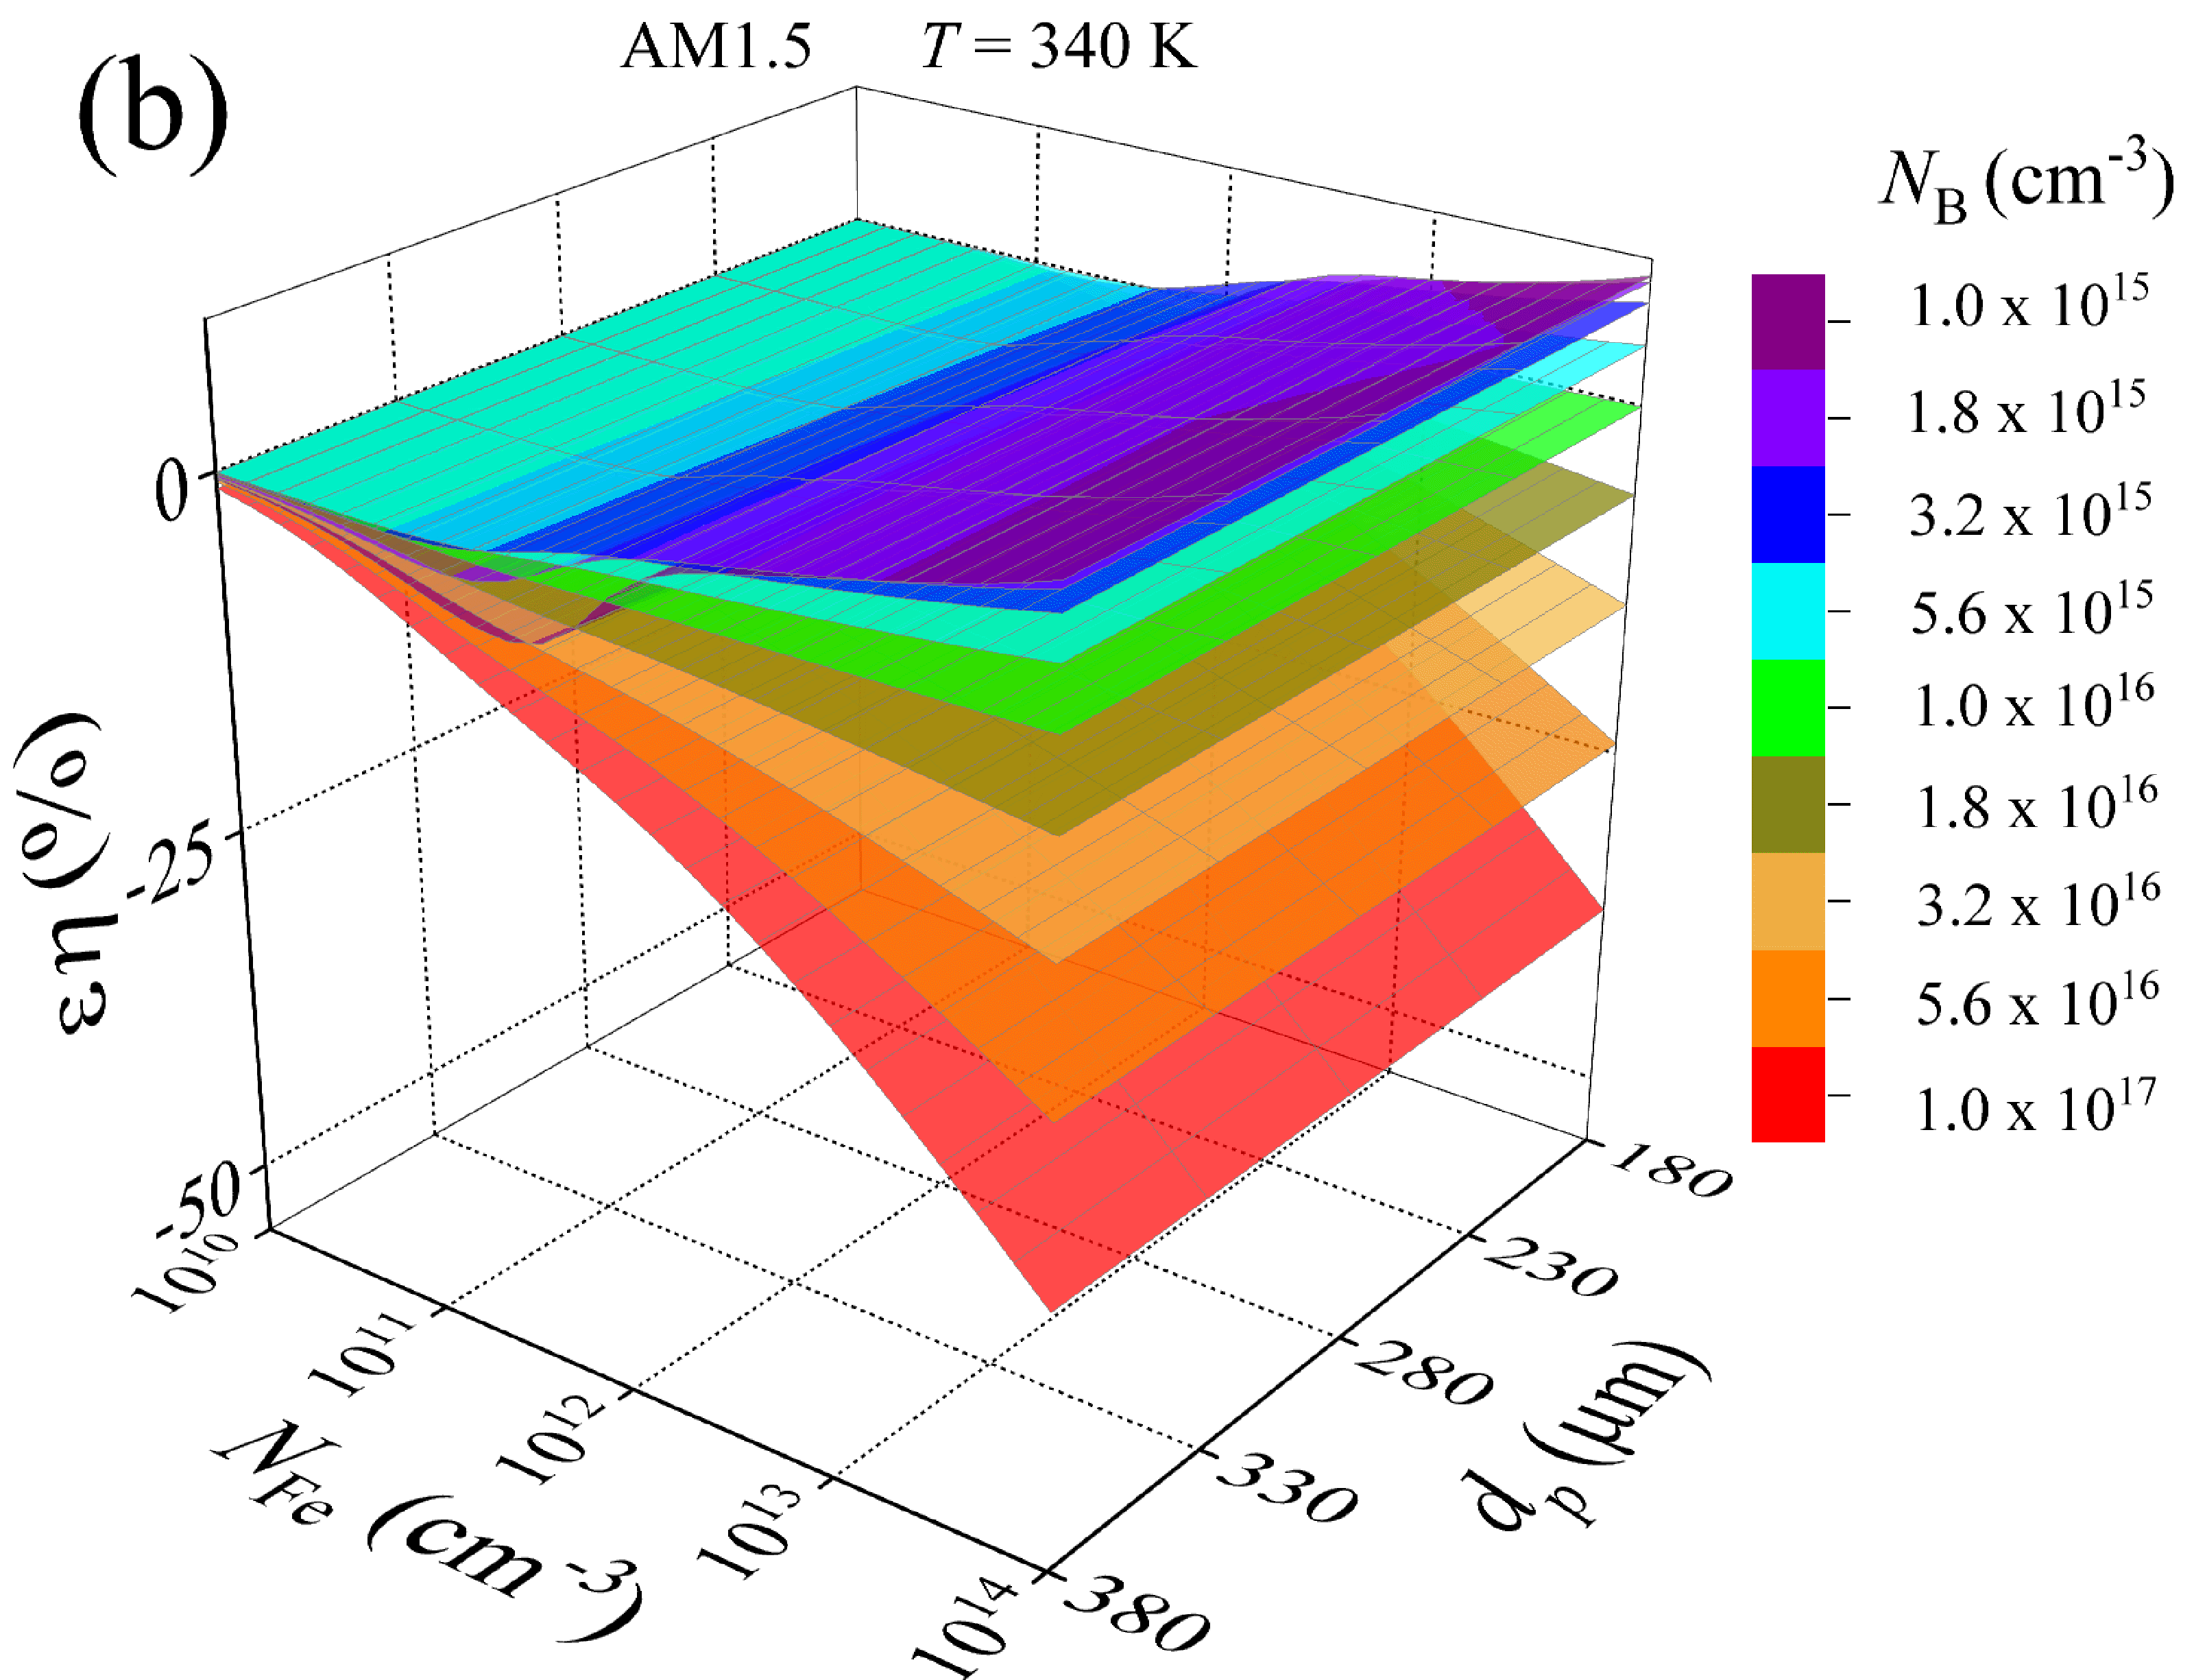
\includegraphics[width=0.49\linewidth]{Fig10b.png}
     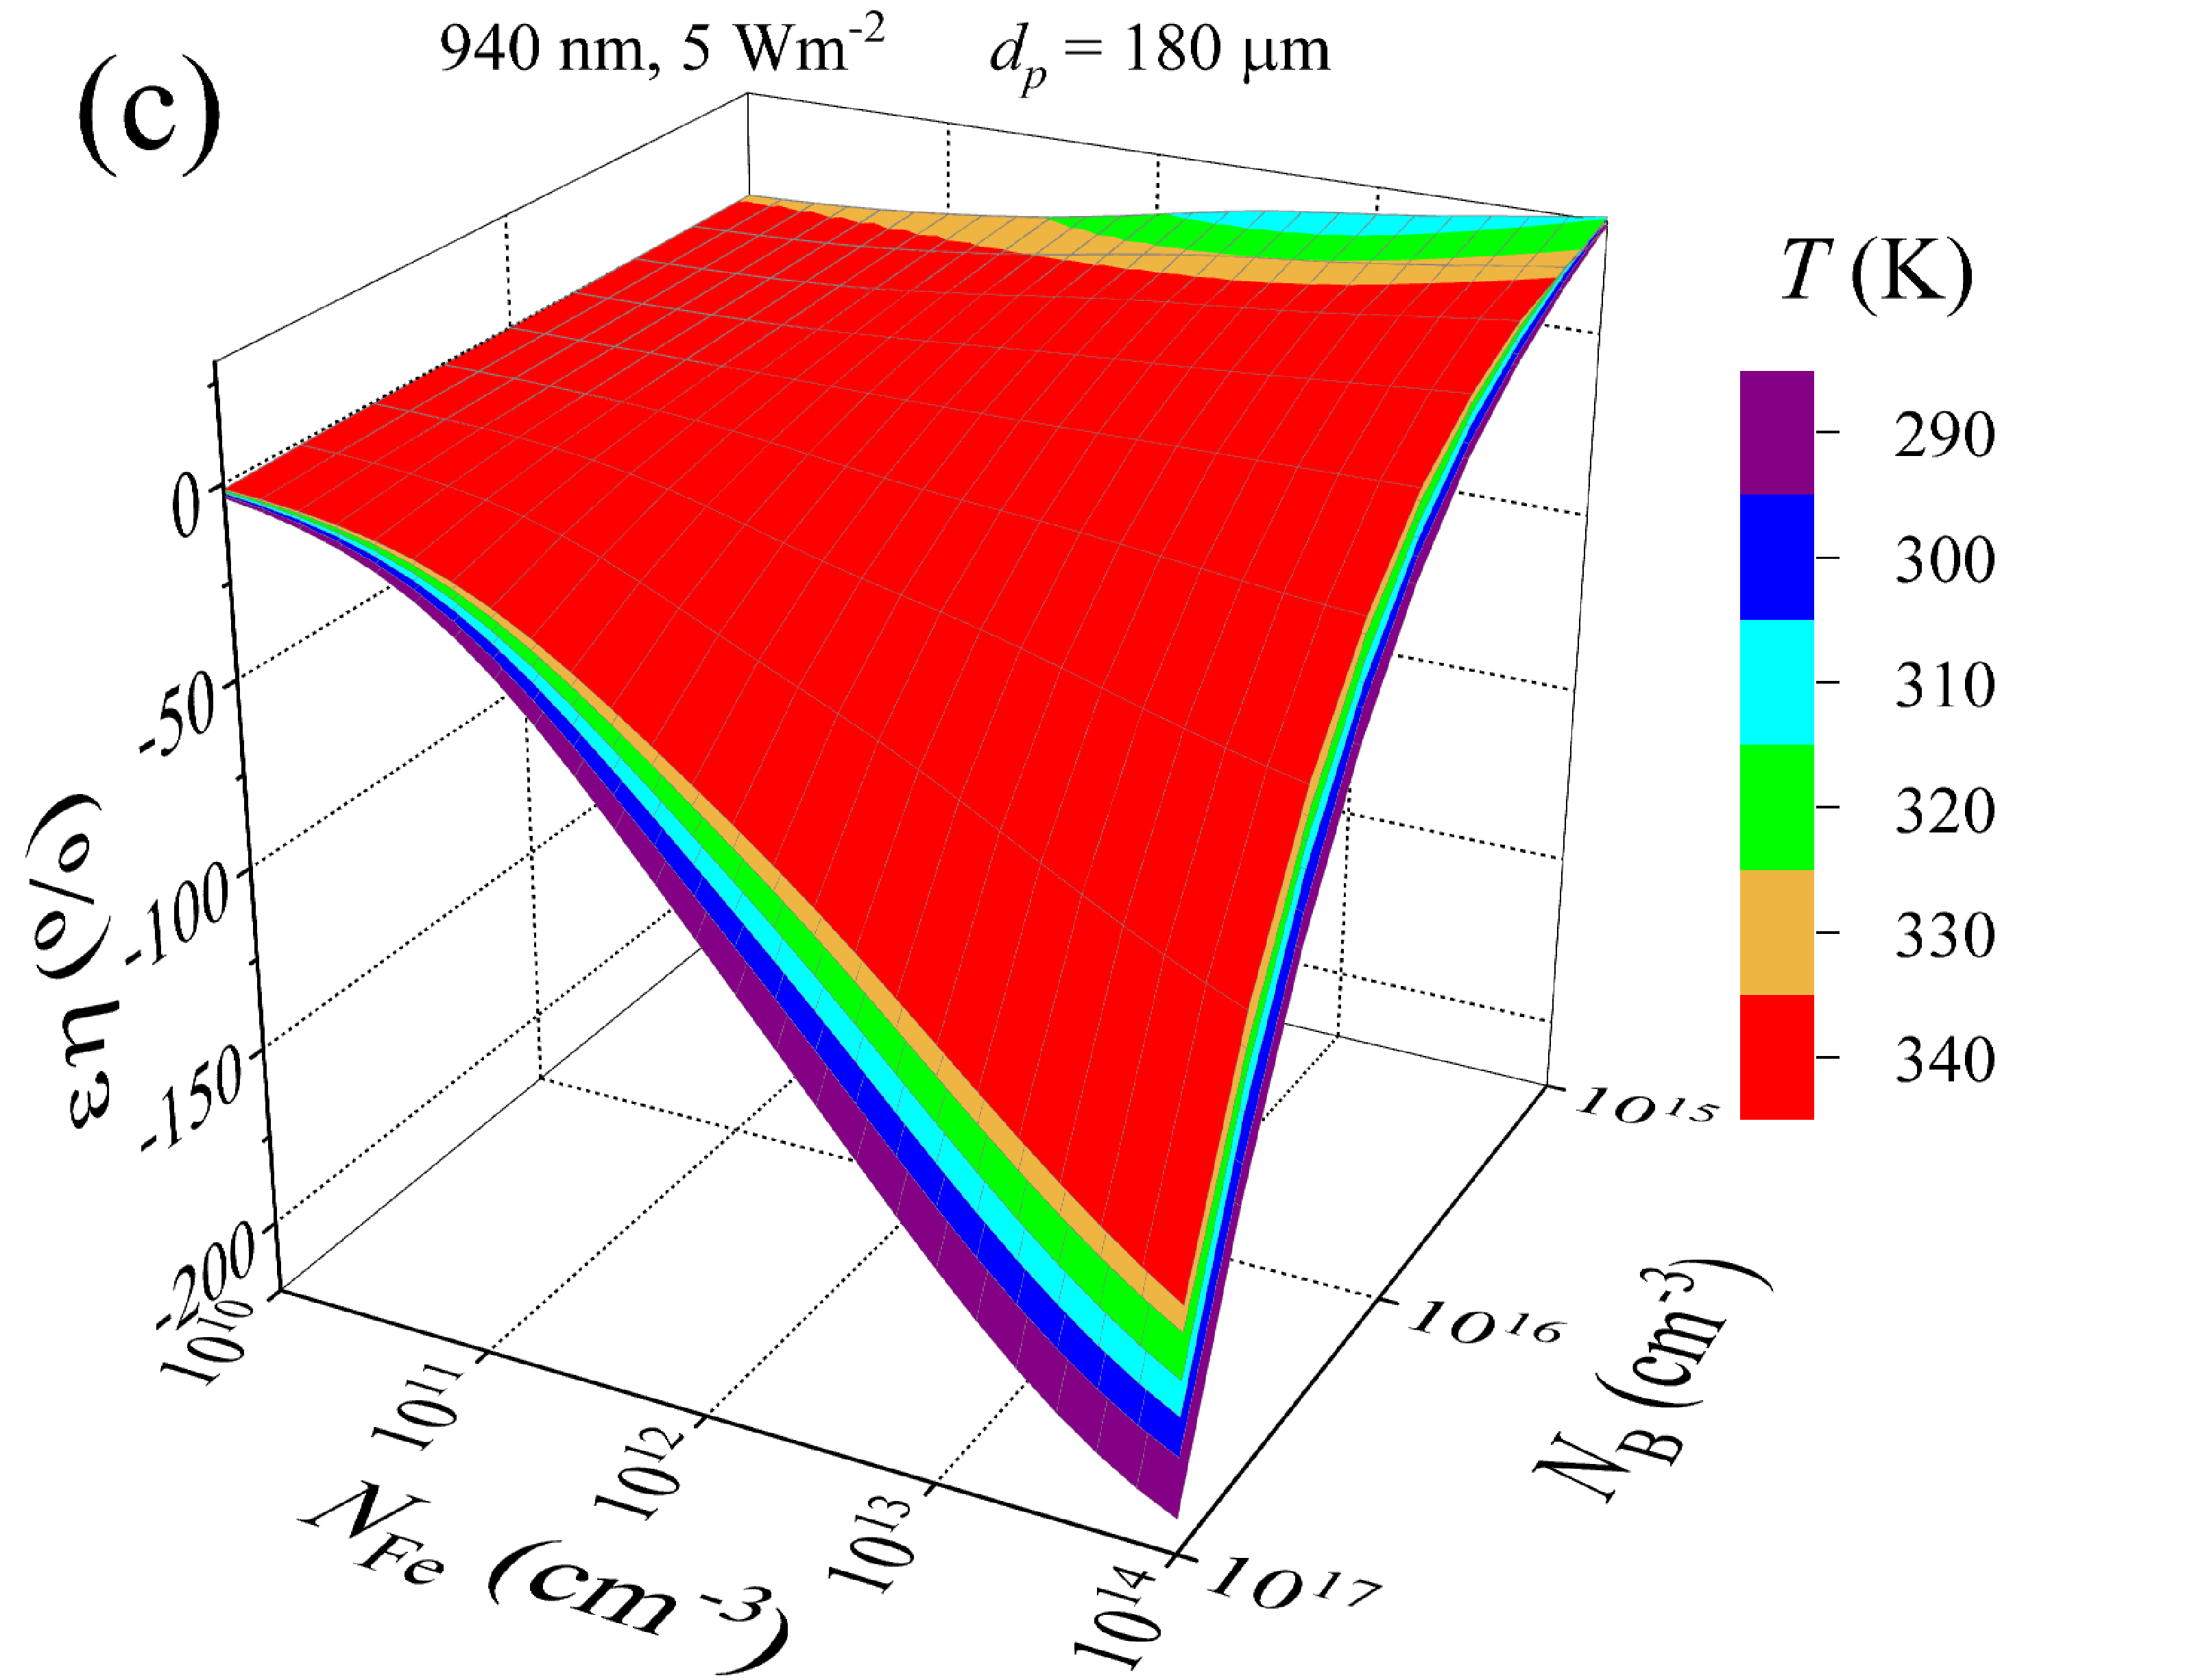
\includegraphics[width=0.49\linewidth]{Fig10c.png}
     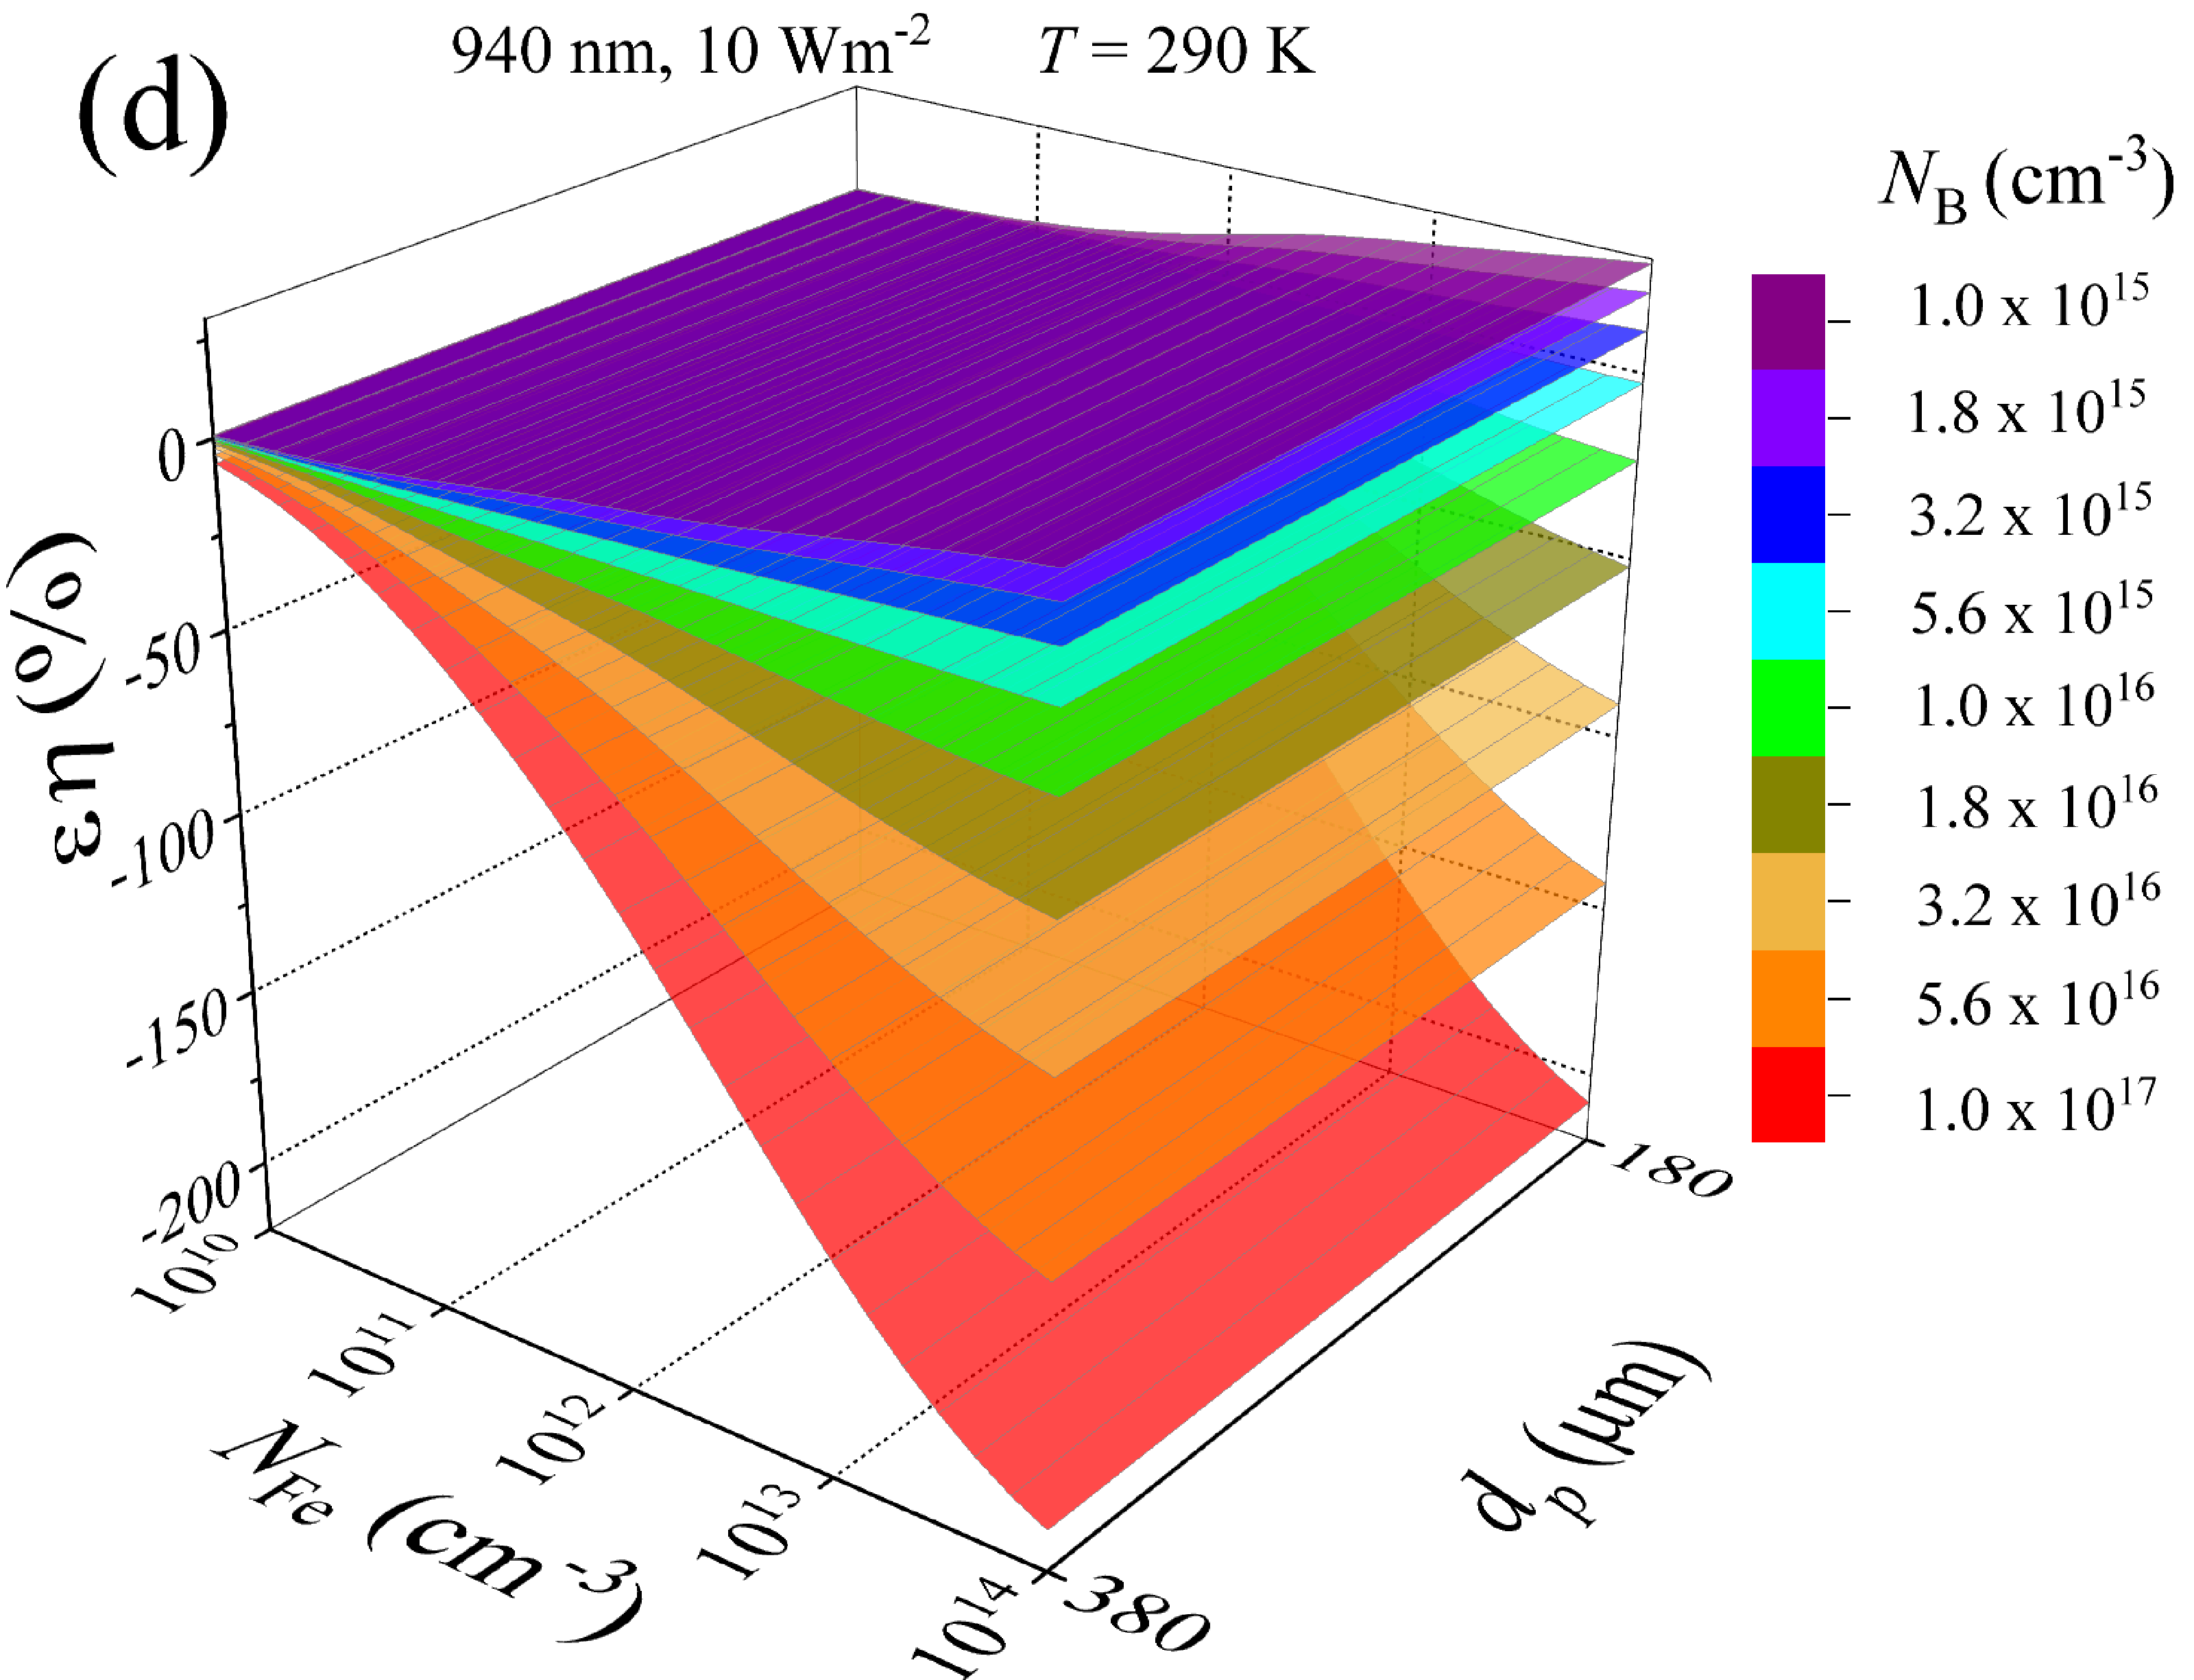
\includegraphics[width=0.49\linewidth]{Fig10d.png}
	  \caption{Relative changes in SSC efficiency caused by a complete
       dissociation of Fe$_i$B$_s$ pairs as a function of
       iron concentration and
       doping level (panels a and c) or base depth (b, d).
       Illumination: AM1.5 (a, b), 940~nm 5~Wm$^{-2}$ (c),  940~nm 10~Wm$^{-2}$ (d).
       $T$, K: 290 (d), 340 (b).
       $d_p$, $\mu$m: 180 (a, c).
       Different surfaces correspond to different temperatures (a, c) and doping levels (b, d).
}\label{fig10}
\end{figure}


\begin{figure}
	\centering
     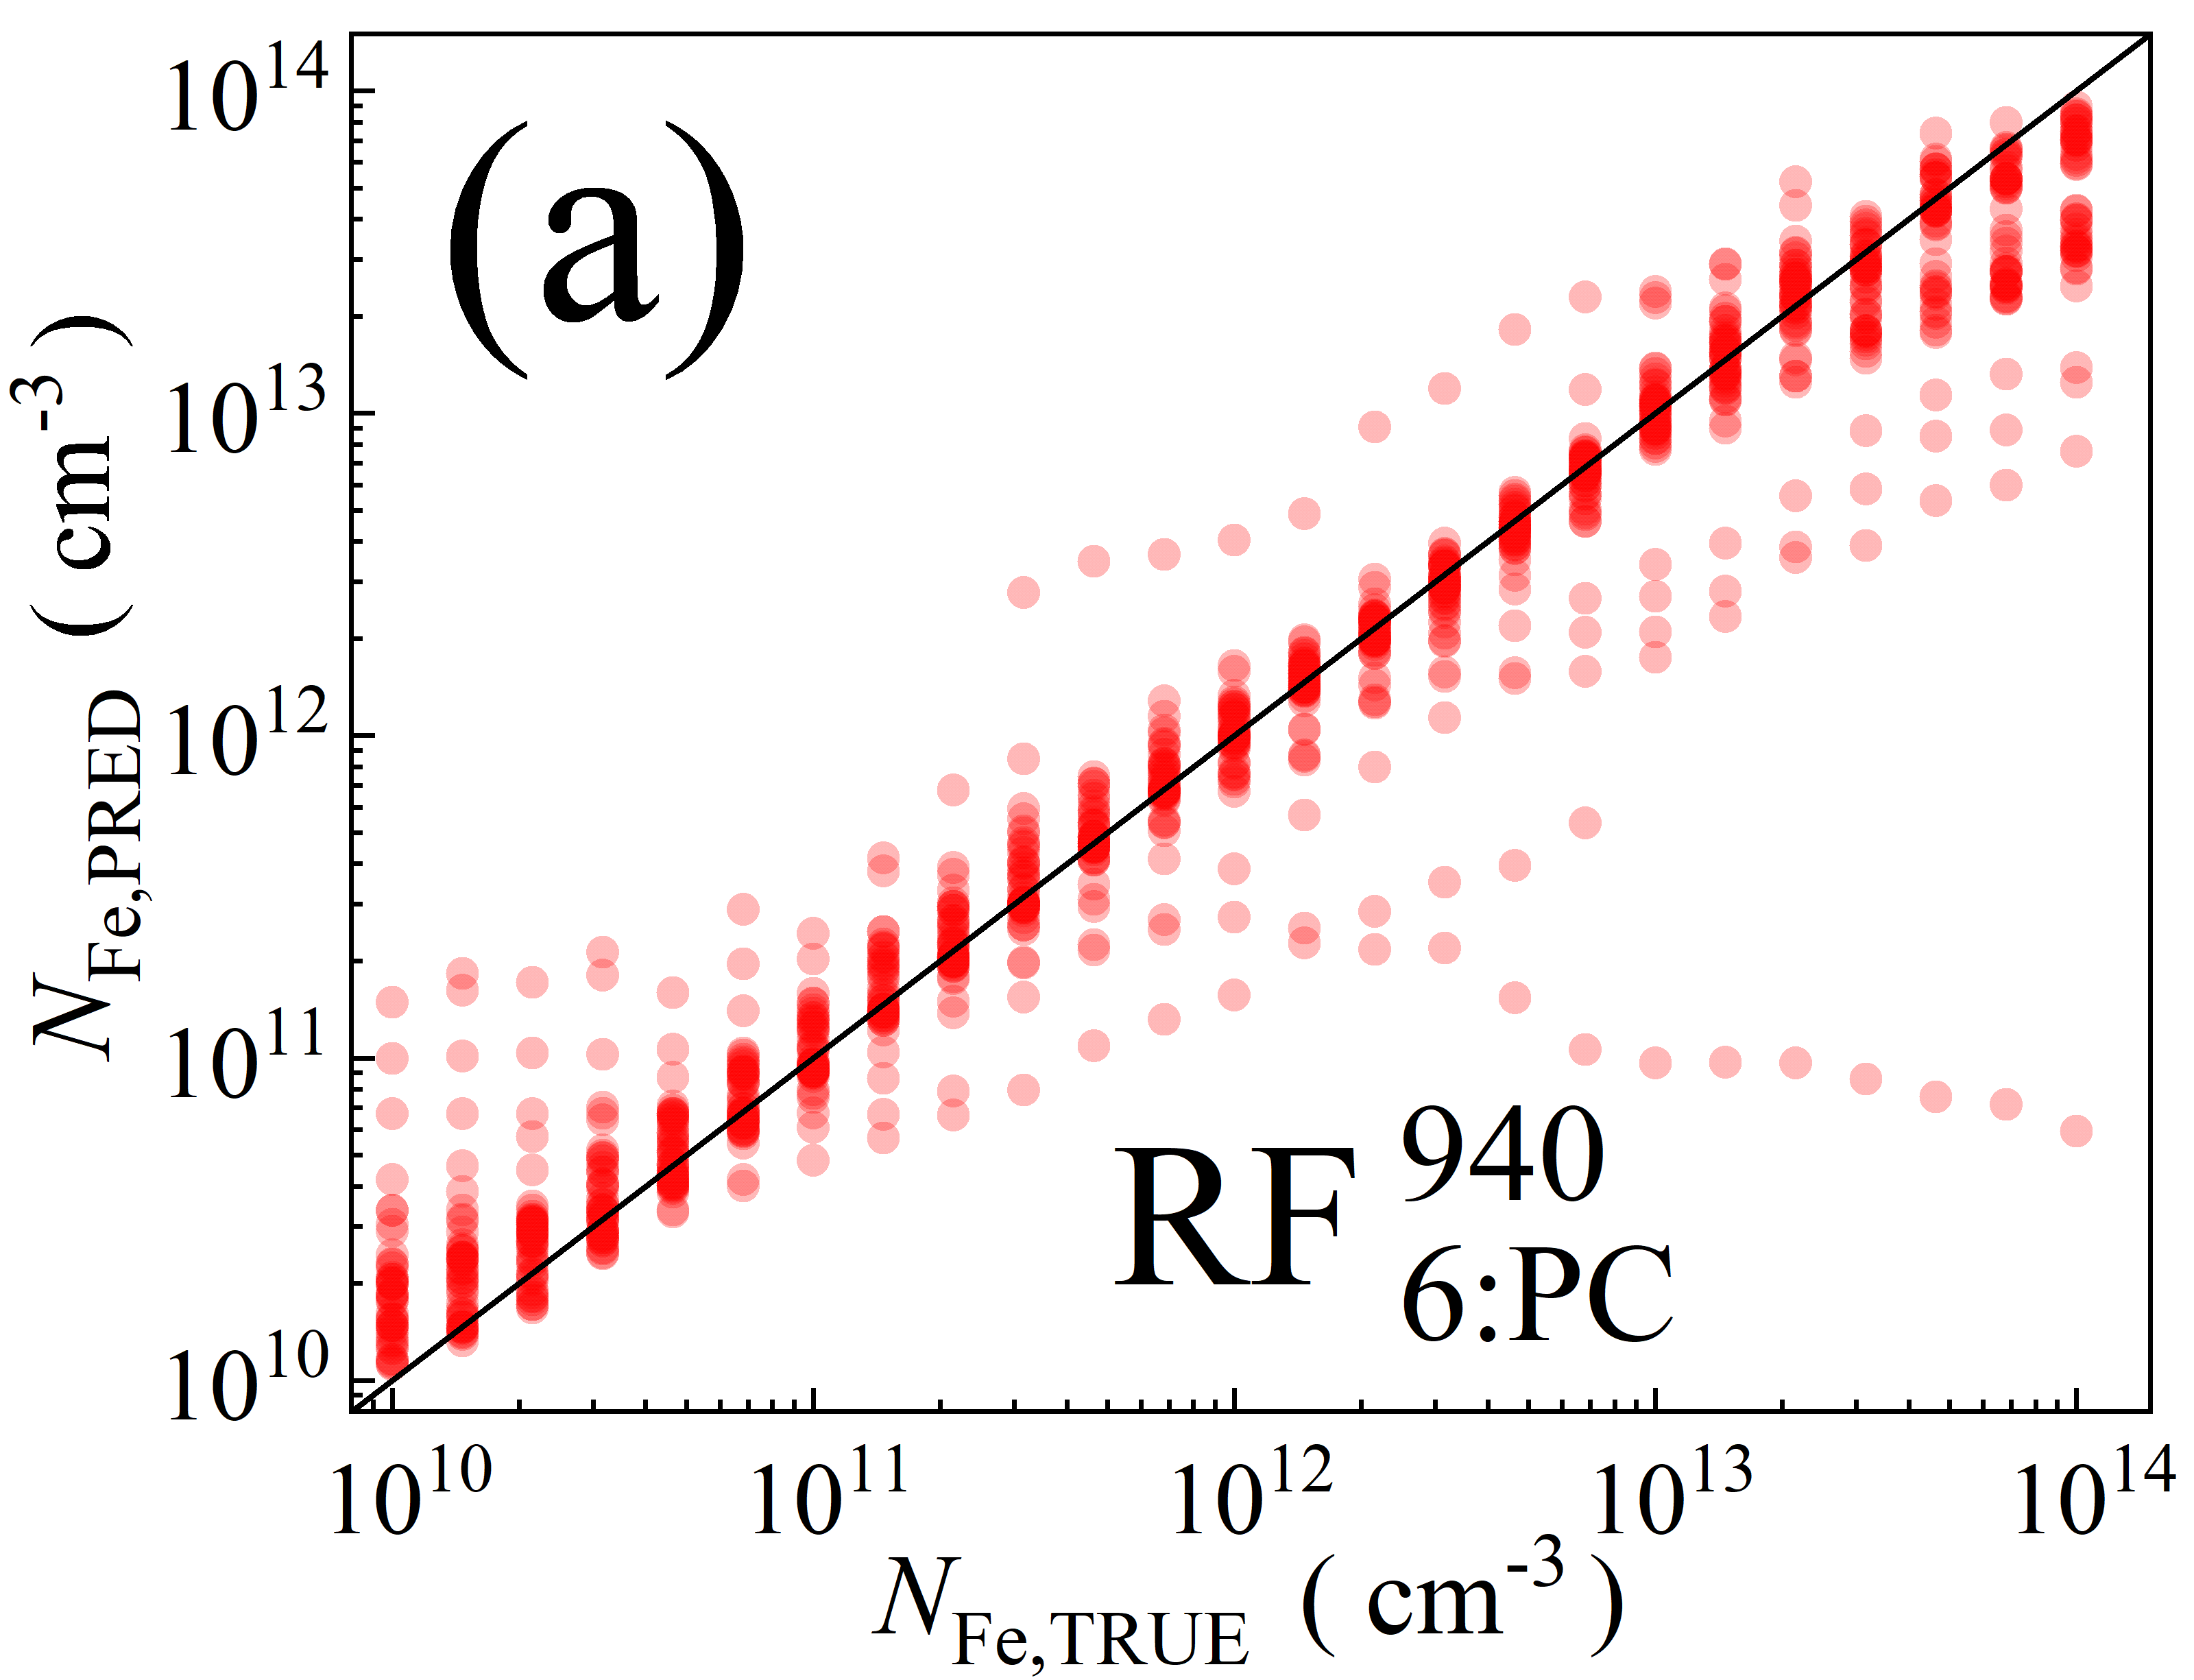
\includegraphics[width=0.4\linewidth]{Fig11a.png}
     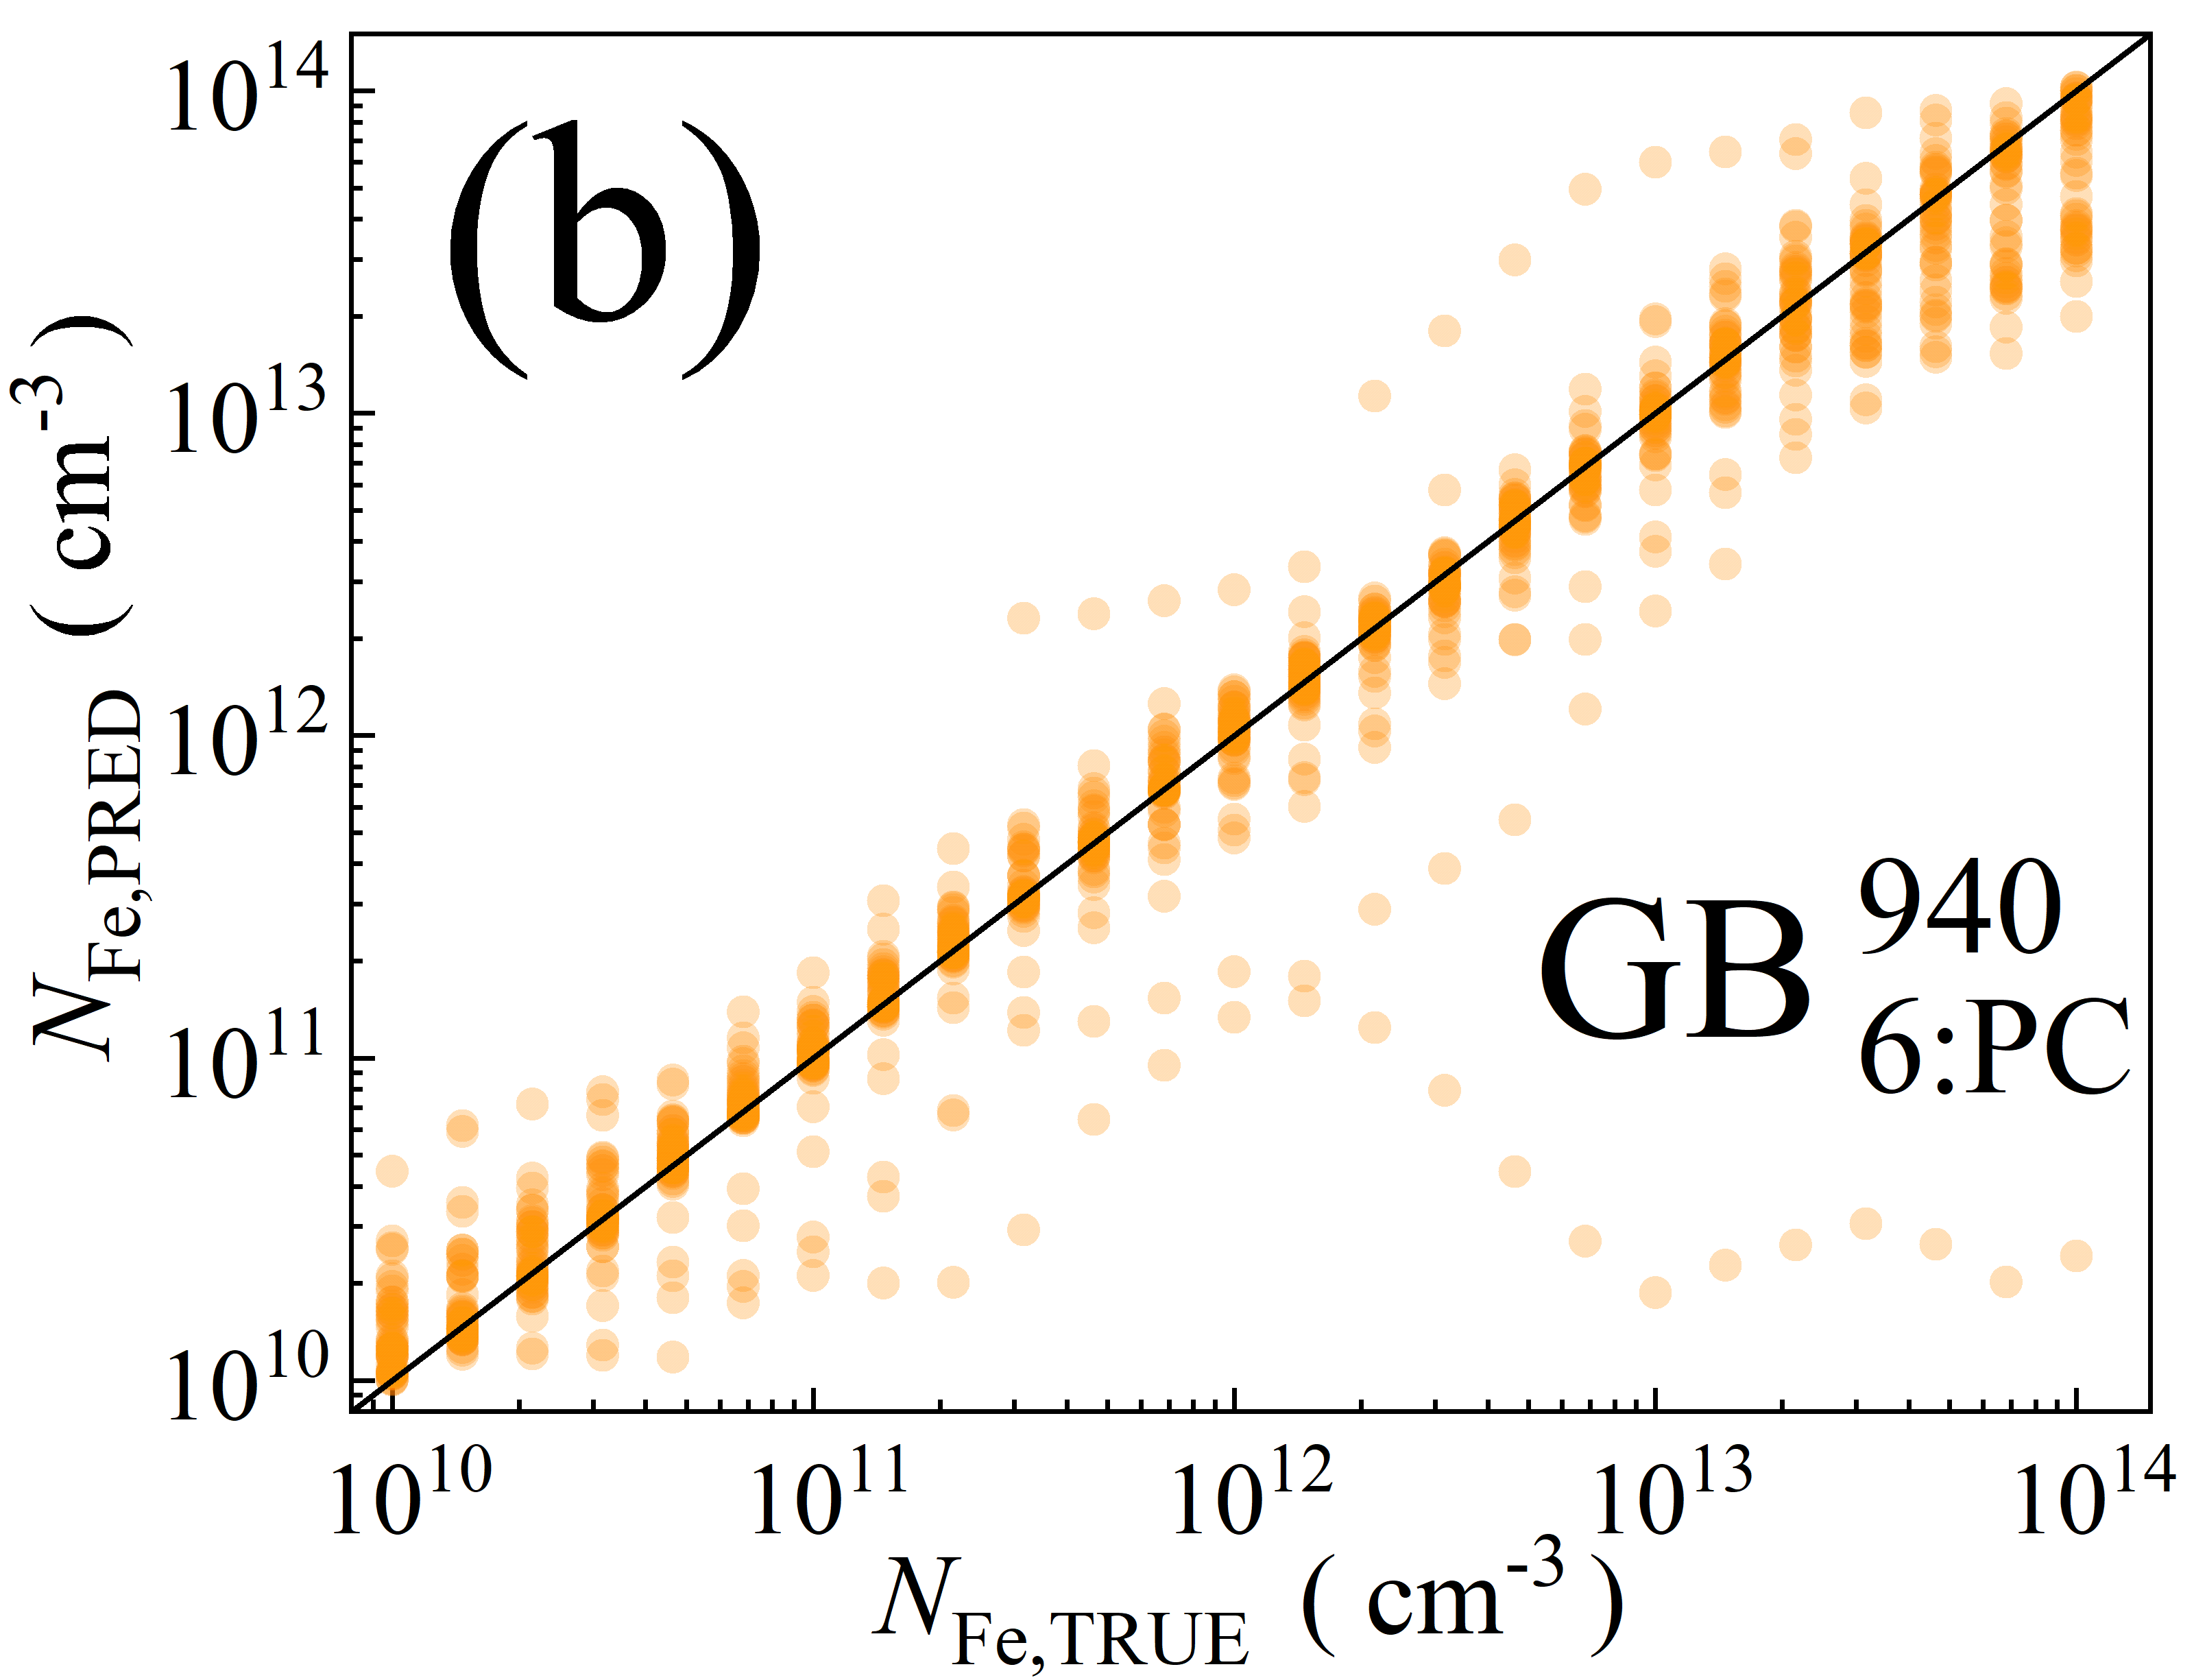
\includegraphics[width=0.4\linewidth]{Fig11b.png}
	  \caption{Relative changes in SSC efficiency caused by a complete
       dissociation of Fe$_i$B$_s$ pairs as a function of iron concentration (a) and
       temperature (b) for SSC with $d_p=380$~$\mu$m and $N_\mathrm{B}=1.36\times10^{15}$~cm$^{-3}$
       in the case of monochromatic (940~nm) illumination.
       The marks are the experimental results (divided by factor $C_{cor}=1.4$), the lines are the simulation results.
       $W_\mathrm{ill}$, Wm$^{-2}$: 5 (marks and solid lines), 10 (dotted lines).
       Different lines and marks correspond to different temperatures (a) or $N_\mathrm{Fe}$ values (b) --- see legends.
}\label{fig11}
\end{figure}

\section{Conclusion}

The paper presents the results of modeling the impact of variations in the state of iron impurities on the photovoltaic parameters of silicon solar cells with different base parameters under various external conditions (temperature, spectral composition of illumination, and intensity). The simulation results have been compared with experimental data.

The feasibility of using relative changes in short-circuit current, open-circuit voltage, fill factor, and efficiency resulting from the dissociation of FeB pairs for estimating the concentration of iron impurities in a solar cell has been analyzed. It is shown that the most suitable parameter for addressing this task is the changes in short-circuit current. Moreover, using monochromatic illumination with a wavelength predominantly absorbed in the depth of the base is more appropriate than AM1.5. Next in suitability are changes in efficiency and open-circuit voltage, although there are limitations to their use at low ($<10^{16}$~cm$^{-3}$) doping levels of the base. In our opinion, using the fill factor to estimate iron concentration is impractical.

It has been shown that the potential accuracy of estimating iron concentration depends on the doping level of the base: at a boron concentration around $<10^{16}$~cm$^{-3}$, it is minimal while decreasing or increasing this value enhances the response of the $I_\mathrm{SC}$ to the presence of iron. Furthermore, the accuracy of the $N_\mathrm{Fe}$ determination is significantly influenced by the availability of precise information on the doping level of the base, as well as the accuracy of estimating the intensity of monochromatic illumination (when using $\varepsilon \eta$ and especially $\varepsilon V_\mathrm{OC}$).

At the same time, $\varepsilon \eta$ and $\varepsilon V_\mathrm{OC}$ can serve as additional refining parameters for determining iron concentration. It is known that in machine learning, the input parameters typically consist of a set of several descriptors. In our view, for the task of estimating iron concentration through changes in photovoltaic parameters during the conversion of iron-containing defects, it is advisable to use a set of ($T$, $d_p$, $N_\mathrm{B}$, $\varepsilon I_\mathrm{SC}$, $\varepsilon \eta$) or ($T$, $d_p$, $N_\mathrm{B}$, $\varepsilon I_\mathrm{SC}$, $\varepsilon \eta$,$\varepsilon V_\mathrm{OC}$).
%--------------------------------------------------------


% Numbered list
% Use the style of numbering in square brackets.
% If nothing is used, default style will be taken.
%\begin{enumerate}[a)]
%\item
%\item
%\item
%\end{enumerate}

% Unnumbered list
%\begin{itemize}
%\item
%\item
%\item
%\end{itemize}

% Description list
%\begin{description}
%\item[]
%\item[]
%\item[]
%\end{description}

% Figure
%\begin{figure}[<options>]
%	\centering
%		\includegraphics[<options>]{}
%	  \caption{}\label{fig1}
%\end{figure}


%\begin{table}[<options>]
%\caption{}\label{tbl1}
%\begin{tabular*}{\tblwidth}{@{}LL@{}}
%\toprule
%  &  \\ % Table header row
%\midrule
% & \\
% & \\
% & \\
% & \\
%\bottomrule
%\end{tabular*}
%\end{table}

% Uncomment and use as the case may be
%\begin{theorem}
%\end{theorem}

% Uncomment and use as the case may be
%\begin{lemma}
%\end{lemma}

%% The Appendices part is started with the command \appendix;
%% appendix sections are then done as normal sections
%% \appendix

%\section{}\label{}

% To print the credit authorship contribution details
\printcredits

%% Loading bibliography style file
\bibliographystyle{model1-num-names}

%\bibliographystyle{cas-model2-names}

% Loading bibliography database
\bibliography{olikh}

% Biography
%\bio{}
%% Here goes the biography details.
%\endbio
%
%\bio{pic1}
%% Here goes the biography details.
%\endbio

\end{document}

